\documentclass{article}

% if you need to pass options to natbib, use, e.g.:
%     \PassOptionsToPackage{numbers, compress}{natbib}
% before loading neurips_2019

% ready for submission
% \usepackage{neurips_2019}

% to compile a preprint version, e.g., for submission to arXiv, add add the
% [preprint] option:
%     \usepackage[preprint]{neurips_2019}

% to compile a camera-ready version, add the [final] option, e.g.:
\usepackage[final]{neurips_2019}

% to avoid loading the natbib package, add option nonatbib:
%     \usepackage[nonatbib]{neurips_2019}

\usepackage{bm}
\usepackage{graphicx}
\usepackage{subcaption}
\usepackage{amsmath}
\usepackage{float}
\usepackage[inline]{enumitem}

\usepackage[utf8]{inputenc} % allow utf-8 input
\usepackage[T1]{fontenc}    % use 8-bit T1 fonts
\usepackage{hyperref}       % hyperlinks
\usepackage{url}            % simple URL typesetting
\usepackage{booktabs}       % professional-quality tables
\usepackage{amsfonts}       % blackboard math symbols
\usepackage{nicefrac}       % compact symbols for 1/2, etc.
\usepackage{microtype}      % microtypography
\usepackage{bbold}
\usepackage{wrapfig}
\usepackage{tikz}
\usepackage{xspace}
\usetikzlibrary{shapes,snakes, arrows}

\newcommand\Simplex{S}
\newcommand\History{\mathcal{H}}
\newcommand\Event{e}
\newcommand\Input{x}
\newcommand\Class{c}
\newcommand\Timestamp{t}
\newcommand\DeltaTime{\tau}
\newcommand\DistParam{\theta}
\newcommand\NbEvents{n}
\newcommand\IndexEvent{i}
\newcommand\NbClasses{C}
\newcommand\IndexClass{c}
\newcommand\NbPoints{M}
\newcommand\IndexPoint{j}

\newcommand\GPModel{WGP-LN\xspace}
\newcommand\DirModel{FD-Dir\xspace}
\newcommand\UncertaintyLoss{uncertainty cross-entropy\xspace}
\newcommand\TimeScore{Time-Error\xspace}

\newcommand\com[1]{\textcolor{black}{#1}}
\newcommand\sg[1]{\textcolor{blue}{(SG: #1)}}
\newcommand\mb[1]{\textcolor{purple}{(MB) #1}}
\newcommand\bc[1]{\textcolor{red}{(BC) #1}}
%\newcommand\sg[1]{}


\DeclareMathOperator{\E}{\mathbb{E}}
\DeclareMathOperator{\CrossEntropy}{H}

\title{Uncertainty on Asynchronous Time Event Prediction}

% The \author macro works with any number of authors. There are two commands
% used to separate the names and addresses of multiple authors: \And and \AND.
%
% Using \And between authors leaves it to LaTeX to determine where to break the
% lines. Using \AND forces a line break at that point. So, if LaTeX puts 3 of 4
% authors names on the first line, and the last on the second line, try using
% \AND instead of \And before the third author name.

\author{%
  Marin Biloš\thanks{Equal contribution} , Bertrand Charpentier\footnote[1]{} , Stephan Günnemann\\
  Technical University of Munich, Germany\\
  \texttt{\{bilos, charpent, guennemann\}@in.tum.de}
}

\begin{document}

\maketitle

\begin{abstract}
Asynchronous event sequences are the basis of many applications throughout different industries. In this work, we tackle the task of predicting the next event (given a history), and how this prediction changes with the passage of time. Since at some time points (e.g.\ predictions far into the future) we might not be able to predict anything with confidence, capturing uncertainty in the predictions  is crucial. We present two new architectures, \GPModel and \DirModel, modelling the evolution of the distribution on the probability simplex with time-dependent logistic normal and Dirichlet distributions. In both cases, the combination of RNNs with either Gaussian process or function decomposition allows to express rich temporal evolution of the distribution parameters, and naturally captures uncertainty. Experiments on class prediction, time prediction and anomaly detection demonstrate the high performances of our models on various datasets compared to other approaches.
\end{abstract}


\section{Introduction}
%\label{sec:introduction_008}

% \looseness=-1
% Safety is critical to the adoption of deep learning in domains such as autonomous driving, medical diagnosis, or financial trading systems. A solution for this problem is to create reliable models capable to estimate the uncertainty of its own predictions. 
% Different uncertainty types are divided in \textit{aleatoric} uncertainty quantified by the inherited noise in the data, thus irreducible; \textit{epistemic} uncertainty quantified by the modeling choice or lack of data, thus reducible; \textit{predictive} uncertainty, a combination of aleatoric and epistemic \citep{gal2016uncertainty}. 
% In practice, high quality uncertainty estimates must be calibrated and able to detect Out-Of-Distribution (OOD) data like anomalies while preserving good Out-Of-Distribution (OOD) generalization performances like on dataset shifts.

While we have focused in the previous sections on proposing new Bayesian models for efficient uncertainty estimation on independent data, we now turn our attention on the practical considerations when using efficient uncertainty estimation methods. 

Recently, a family of methods for uncertainty estimation named Deterministic Uncertainty Methods (DUMs) have emerged \citep{postels2022practicalitydum}. 
Contrary to uncertainty methods such as Ensembles \citep{ensembles}, MC Dropout \citep{dropout} or other Bayesian neural networks on weights \citep{bayesian-networks}, which require multiple forward passes to make predictions, DUMs only require a single forward pass, thus making them significantly more computationally efficient. 
%These models can make predictions in only a single forward pass,  %thus being computationally efficient. 
Generally, DUMs are composed of three components with high potential impact on their performances: the \emph{training} procedure which is supposed to optimize the model toward high predictive and uncertainty performances,  the core \emph{architecture} which is supposed to define informative embeddings used to make predictions, and the \emph{prior} which is supposed to define the default uncertain predictions. In this work, we investigate the role of these three components on the quality of DUMs uncertainty estimates by evaluating calibration performances, OOD detection, and OOD generalization. Our main contributions are:
\vspace{-2mm}
\begin{itemize}
%\setlength\itemsep{-1mm}
    \item \textbf{Training}: We show that \emph{decoupling the learning rates} of the core architecture and uncertainty heads of DUMs, \emph{jointly training} the core architecture and the uncertainty head of DUMs, and \emph{pretraining} with \emph{more data} and \emph{higher data quality} improve uncertainty performances. 
    \item \textbf{Architecture}: We demonstrate that the expressiveness of the core architecture defined by the \emph{architecture type}, \emph{architecture size}, and \emph{dimension of the latent space} is crucial for \emph{both} predictive and uncertainty performances. Further, we show that applying additional regularization constraints to avoid \emph{feature collapse} does not find better trade-off between OOD detection and generalization, even sometimes degrading performances.
    \item \textbf{Prior}: In contrast to Bayesian neural networks on weights where the choice of prior is critical \citep{bayesposterior2020wenzel, fortuin2022prior, noci2021prior_cpe, kapoor2022prior_cpe}, we empirically show that the choice of prior defined in the training loss or in the uncertainty head of DUMs has a relatively small effect on the final uncertainty performances.
\end{itemize}

\section{Model Description}
\label{sec:model_010}

We consider a sequence $[e_1,\ldots, e_n]$ of events $\Event_\IndexEvent = (\Class_\IndexEvent, \Timestamp_\IndexEvent)$, where $\Class_\IndexEvent\in \{1,\ldots,\NbClasses\}$ denotes the class of the $\IndexEvent$th event and $\Timestamp_\IndexEvent\in \mathbb{R}$ is its time of occurrence. We assume the events arrive over time, i.e.\ $t_{\IndexEvent}>t_{\IndexEvent-1}$, and we introduce $\DeltaTime^*_\IndexEvent = \Timestamp_\IndexEvent - \Timestamp_{\IndexEvent-1}$ as the observed time gap between the $\IndexEvent$th and the $(\IndexEvent-1)$th event. The history preceding the $\IndexEvent$th event is denoted by $\History_{\IndexEvent}$.
Let $\Simplex=\{\bm{p} \in [0,1]^\NbClasses, \sum_\IndexClass p_\IndexClass = 1\}$ denote the set of probability vectors that form the $(\NbClasses-1)$-dimensional simplex, and $P(\theta)$ be a family of probability distributions on this simplex parametrized by parameters $\theta$. Every sample $\bm p \sim P(\theta)$ corresponds to a (categorical) class distribution.

Given $\Event_{\IndexEvent-1}$ and $\History_{\IndexEvent-1}$, our goal is to model the evolution of the class probabilities, and their uncertainty, of the next event $\IndexEvent$ over time. Technically, we model parameters $\theta(\DeltaTime)$, leading to a distribution $P$ over the class probabilities $\bm p$ for all $\DeltaTime \geq 0$. Thus, we can estimate the most likely class after a time gap $\DeltaTime$ by calculating $\arg\!\max_c \bm{\bar p}(\DeltaTime)_c$, where $\smash{\bm{\bar p}(\DeltaTime) := \E_{\bm p(\DeltaTime) \sim P(\theta(\DeltaTime))}[\bm p(\DeltaTime)]}$ is the expected probability vector. Even more, since we do not consider a point estimate, we can get the amount of certainty in a prediction. For this, we estimate the probability of class $\IndexClass$ being more likely than the other classes, given by $\smash{q_\IndexClass(\DeltaTime) := \E_{\bm p(\DeltaTime) \sim P(\theta(\DeltaTime))}[\mathbb{1}_{\bm p(\DeltaTime)_\IndexClass \geq  \max_{c'\neq c} \bm p(\DeltaTime)_{c'}}]}$. This tells us how certain we are that one class is the most probable (i.e.\ 'how often' is $c$ the argmax when sampling from $P$).

Two expressive and well-established choices for the family $P$ are the Dirichlet distribution and the logistic-normal distribution (\cref{distributions}). Based on a common modeling idea, we present two models that exploit the specificities of these distributions: the \GPModel (\cref{GP}) and the \DirModel (\cref{dirichlet}). We also introduce a novel loss to train these models in \cref{uncertainty_loss}.

Independent of the chosen model, we have to tackle two core challenges: (1) \textbf{Expressiveness.} Since the time dependence of $\theta(\DeltaTime)$ may be of different forms, we need to capture complex behavior. (2) \textbf{Locality.} For regions out of the observed data we want to have a higher uncertainty in our predictions. Specifically for $\DeltaTime \rightarrow \infty$, i.e.\  far into the future, the distribution should have a high uncertainty.


\subsection{Logistic-Normal via a Weighted Gaussian Process (\GPModel)}
\label{GP}

\begin{figure}
	\centering
	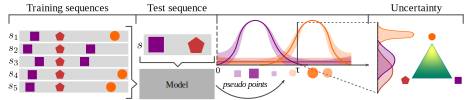
\includegraphics[width=\linewidth]{sections/010_neurips2019/paper/images/model_schema.pdf}
	\begin{subfigure}{0.3\textwidth}
		\caption{} \label{fig:model_illustration_1}
	\end{subfigure}
	\begin{subfigure}{0.69\textwidth}
		\caption{} \label{fig:model_illustration_2}
	\end{subfigure}
	\vspace*{-0.5cm}
    \caption{The model framework. (a) During training we use sequences $s_i$. (b) Given a new sequence of events $s$ the model generates pseudo points that describe $\bm{\theta}(\DeltaTime)$, i.e. the temporal evolution of the distribution on the simplex. These pseudo points are based on the data that was observed in the training examples and weighted accordingly. We also have a measure of certainty in our prediction.}\label{fig:model_illustration}
    \vspace*{-0.5cm}
\end{figure}

We start by describing our model for the case when $P$ is the family of logistic-normal (LN) distributions.
How to model a compact yet expressive evolution of the LN distribution?
Our core idea is to exploit the fact that the LN distribution corresponds to a multivariate random variable whose \textit{logits} follow a \textit{normal distribution} -- and a natural way to model the evolution of a normal distribution is a \textit{Gaussian Process}. Given this insight, the core idea of our model is illustrated in Fig. \ref{fig:model_illustration}: (1) we generate $\NbPoints$ pseudo points based on a hidden state of an RNN whose input is a sequence, (2) we fit a Gaussian Process to the pseudo points, thus capturing the temporal evolution, and (3) we use the learned GP for estimating the parameters $\bm \mu(\DeltaTime)$ and $\bm \Sigma(\DeltaTime)$ of the final LN distribution at any specific time $\tau$. Thus, by generating a small number of points we characterize the full distribution.

\paragraph{Classic GP.}  To keep the complexity low, we train one GP per class $\IndexClass$. That is, our model generates $\NbPoints$ points $(\DeltaTime_\IndexPoint^{(\IndexClass)}, y_\IndexPoint^{(\IndexClass)})$ per class $\IndexClass$, where $y_\IndexPoint^{(\IndexClass)}$ represents logits. Note that the first coordinate of each pseudo point corresponds to time, leading to the temporal evolution when fitting the GP. Essentially we perform a non-parameteric regression from the time domain to the logit space. Indeed, using a classic GP along with the pseudo points, the parameters $\theta$ of the logistic-normal distribution, $\bm \mu$ and $\bm \Sigma$, can be easily computed for any time $\tau$ in closed form:
\begin{equation}\label{eq:gp_prediction}
\begin{aligned}
\mu_{\IndexClass}(\DeltaTime) = \bm{k}_{\IndexClass}^T \bm{K}_{\IndexClass}^{-1} \bm{y}_{\IndexClass},\
\sigma_{\IndexClass}^2(\DeltaTime) = s_{\IndexClass} - \bm{k}_{\IndexClass}^T \bm{K}_{\IndexClass}^{-1} \bm{k}_{\IndexClass}
\end{aligned}
\end{equation}
where  $\bm K_c$ is the  gram matrix w.r.t.\ the $M$ pseudo points of class $c$ based on a  kernel $k$ (e.g. $\smash{k(\DeltaTime_1, \DeltaTime_2) = \exp( -\gamma^2 (\DeltaTime_1 - \DeltaTime_2)^2)}$). Vector $\bm{k}_{\IndexClass}$ contains at position $j$ the value $\smash{k(\DeltaTime_\IndexPoint^{(\IndexClass)},\tau)}$, and $\bm{y}_{\IndexClass}$ the value $\smash{y_\IndexPoint^{(\IndexClass)}}$, and $s_{\IndexClass}=k(\DeltaTime, \DeltaTime)$. At every time point $\DeltaTime$ the logits then follow a multivariate normal distribution with mean $\bm \mu(\DeltaTime)$ and covariance $\smash{\bm \Sigma = \text{diag}(\bm \sigma^2(\DeltaTime))}$.

Using a GP enables us to describe complex functions. Furthermore, since a GP models uncertainty in the prediction depending on the pseudo points, uncertainty is higher in areas far away from the pseudo points. Specifically, it holds for distant future; thus, matching the idea of locality.
%
However, uncertainty is always low around the $M$ pseudo points. Thus $\NbPoints$ should be carefully picked since there is a trade-off between having high certainty at (too) many time points and the ability to capture complex behavior. Thus, in the following we present an extended version solving this problem.

%\begin{wrapfigure}{r}{7cm}
\begin{figure}
	%\vspace*{-0.5cm}
    \centering
    \includegraphics[width=0.8\linewidth]{sections/010_neurips2019/paper/images/weighted_gaussian_process.pdf}
	\caption{WGP on toy data with different weights. (a) All weights are 1 -- classic GP. (b) Zero weights discard points. (c) Mixed weight assignment.}
	\label{fig:weighted_gaussian_process}
%\vspace*{-0.5cm}
\end{figure}
%\end{wrapfigure}

%%%%% Horizontal %%%%%%
%\begin{figure}[H]
%\centering
%\scalebox{0.9}{\begin{tikzpicture}[
%rectanglenode/.style={rectangle, draw=black!100, very thick, minimum size=10mm},
%roundnode/.style={circle, draw=black!100, very thick, minimum size=10mm},
%nonenode/.style={rectangle, draw=none, minimum size=6mm},
%]
%\tikzset{edge/.style = {->,> = latex'}}
%\node[nonenode] (H)         at (-5.9, 10.25)       {$\History$};
%\node[nonenode] (e)      at (-5.9, 9.75)       {$e$};
%\node[rectanglenode] (RNN)       at (-4.5, 10)       {RNN};
%\node[nonenode] (pi)        at (-3, 9.5)       {$w_\IndexPoint^{(\IndexClass)}$};
%\node[nonenode] (mu)       at (-3, 10)       {$\DeltaTime_\IndexPoint^{(\IndexClass)}$};
%\node[nonenode] (sigma)        at (-3,10.5)       {$y_\IndexPoint^{(\IndexClass)}$};
%\node[nonenode] (alpha)        at (-1.5, 10)       {$\theta(\DeltaTime)$};
%\node[nonenode] (p)        at (0.75, 10)       {$\bm{p}(\DeltaTime) \sim P(\theta(\DeltaTime))$};
%\draw[edge] (H) -> (RNN) {};
%\draw[edge] (e) -> (RNN) {};
%\draw[edge] (RNN) -> (pi) {};
%\draw[edge] (RNN) -> (mu) {};
%\draw[edge] (RNN) -> (sigma) {};
%\draw[edge] (pi) -> (alpha) {};
%\draw[edge] (mu) -> (alpha) {};
%\draw[edge] (sigma) -> (alpha) {};
%\draw[edge] (alpha) -> (p) {};
%\end{tikzpicture}}
%\caption{Model diagram. Both models output pseudo points given history and new event. In \GPModel they generate parameters $\theta(\DeltaTime) = \{\bm \mu (\DeltaTime), \bm \Sigma(\DeltaTime)\}$ that model $P(\theta(\DeltaTime))$ as a logistic-normal distribution. In \DirModel these points generate $\theta(\DeltaTime) = \bm \alpha(\DeltaTime)$ to model $P(\theta(\DeltaTime))$ as a Dirichlet distribution.}
%\label{fig:model_diagram}
%\end{figure}
%%%%% Vertical %%%%%%
% \InsertBoxR{3}{\parbox{0.3\linewidth}{
\begin{wrapfigure}[12]{r}{3.5cm}
    \vspace*{-0.6cm}
    \centering
    \scalebox{.75}{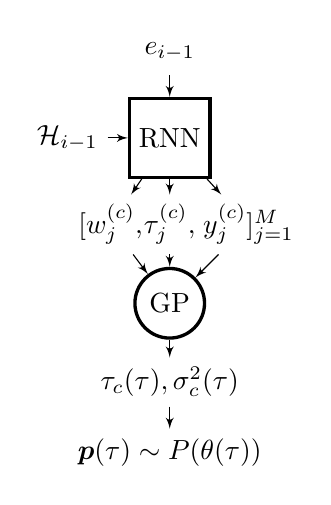
\begin{tikzpicture}[
    rectanglenode/.style={rectangle, draw=black!100, very thick, minimum size=10mm},
    roundnode/.style={circle, draw=black!100, very thick, minimum size=5mm},
    nonenode/.style={rectangle, draw=none, minimum size=6mm},
    ]
    \tikzset{edge/.style = {->,> = latex'}}
    \node[nonenode] (H)         at (8.7,4.5)       {$\History_{\IndexEvent-1}$};
    \node[nonenode] (e)      at (10,5.6)       {$e_{\IndexEvent-1}$};
    \node[rectanglenode] (RNN)       at (10,4.5)       {RNN};
    \node[nonenode] (pi)        at (9.25,3.4)       {$[w_\IndexPoint^{(\IndexClass)},$};
    \node[nonenode] (mu)       at (10,3.4)       {$\DeltaTime_\IndexPoint^{(\IndexClass)},$};
    \node[nonenode] (sigma)        at (11,3.4)       {$y_\IndexPoint^{(\IndexClass)}]_{\IndexPoint=1}^\NbPoints$};
    \node[roundnode] (regression)        at (10,2.4)       {GP};
    \node[nonenode] (alpha)        at (10,1.4)       {$\DeltaTime_{\IndexClass}(\DeltaTime), \sigma_{\IndexClass}^2(\DeltaTime)$};
    \node[nonenode] (p)        at (10,0.5)       {$\bm{p}(\DeltaTime) \sim P(\theta(\DeltaTime))$};
    \draw[edge] (H) -> (RNN) {};
    \draw[edge] (e) -> (RNN) {};
    \draw[edge] (RNN) -> (pi) {};
    \draw[edge] (RNN) -> (mu) {};
    \draw[edge] (RNN) -> (sigma) {};
    \draw[edge] (pi) -> (regression) {};
    \draw[edge] (mu) -> (regression) {};
    \draw[edge] (sigma) -> (regression) {};
    \draw[edge] (regression) -> (alpha) {};
    \draw[edge] (alpha) -> (p) {};
    \end{tikzpicture}}
    \caption{Model diagram}\label{fig:model_diagram}
% }}[6]
    %\vspace*{-1cm}
\end{wrapfigure}

\paragraph{Weighted GP.} We would like to pick $\NbPoints$ large enough to express rich multimodal functions and allow the model to discard unnecessary points.
To do this we generate an additional weight vector $\smash{\bm{w}^{(\IndexClass)} \in [0,1]^\NbPoints}$ that assigns the weight $\smash{w_\IndexPoint^{(\IndexClass)}}$ to a point $\smash{\DeltaTime^{(\IndexClass)}_\IndexPoint}$. Giving a zero weight to a point should discard it, and giving $1$ will return the same result as with a classic GP. To achieve this goal, we introduce a new kernel function:
\begin{equation}
\begin{aligned}\label{eq:weighted_kernel}
    k'(\DeltaTime_1, \DeltaTime_2) &= f(w_1, w_2) k(\DeltaTime_1, \DeltaTime_2)
\end{aligned}
\end{equation}
%\parskip 0pt
where $k$ is the same as above. The function $f$ weights the kernel $k$ according to the weigths for $\DeltaTime_1$ and $\DeltaTime_2$.
We require $f$ to have the following properties: (1) $f$ should be a valid kernel over the weights, since then the function $k'$ is a valid kernel as well; (2) the importance of pseudo points should not increase, giving $f(w_1, w_2) \leq \min(w_1,w_2)$; this fact implies that a point with zero weight will be discarded since $f(w_1, 0)=0$ as desired. The function $f(w_1,w_2)=\min(w_1,w_2)$  is a simple choice that fulfills these properties.
In Fig. \ref{fig:weighted_gaussian_process}  we show the effect of different weights when fitting of a GP (see Appendix \ref{gp_min_kernel} for a more detailed discussion of the behavior of the $\min$ kernel).
%\parskip 5pt
To predict $\mu$ and $\sigma^2$ for a new time $\DeltaTime$, we can now simply apply Eq. \ref{eq:gp_prediction} based on the new kernel $k'$, where the weight for the \textit{query} point $\DeltaTime$ is $1$.

To summarize: From a hidden state $\smash{h_\IndexEvent = \text{RNN}(\Event_{\IndexEvent-1}, \History_{\IndexEvent-1})}$ we use a a neural network to generate $\NbPoints$ weighted pseudo points $(w_\IndexPoint^{(\IndexClass)}, \DeltaTime_\IndexPoint^{(\IndexClass)}, x_\IndexPoint^{(\IndexClass)})$ per class $\IndexClass$.
Fitting a Weighted GP to these points enables us to model the temporal evolution of $\smash{\mathcal{N}(\mu_\IndexClass(\DeltaTime), \sigma_\IndexClass^2(\DeltaTime))}$ and, thus, accordingly of the logistic-Normal distribution. Fig. \ref{fig:model_diagram} shows an illustration of this model.
%
Note that the cubic complexity of a GP, due to the matrix inversion, is not an issue since the number $\NbPoints$ is usually small ($<10$), while still allowing to represent rich multimodal functions. Crucially, given the loss defined in Sec.\ \ref{uncertainty_loss}, our model is fully differentiable, enabling us efficient training.



\subsection{Dirichlet via a Function Decomposition (\DirModel)}
\label{dirichlet}

Next, we consider the Dirichlet distribution to model the uncertainty in the predictions. The goal is to model the evolution of the concentrations parameters $\bm{\alpha}=(\alpha_1, \dots,\alpha_\NbClasses)^T$ of the Dirichlet over time. 
Since unlike to the logistic-normal, we cannot draw the connection to the GP, we propose  to decompose the parameters of the Dirichlet distribution with expressive (local) functions in order to allow complex dependence on time. 
 %
Since the concentration parameters $\alpha_\IndexClass(\DeltaTime)$  need to be positive, we propose the following decomposition of $\alpha_\IndexClass(\DeltaTime)$ in the log-space
\begin{equation}\label{eq:fct_dec}
\begin{aligned}
\log \alpha_\IndexClass(\DeltaTime) &= \sum_{\IndexPoint=1}^{\NbPoints} w_\IndexPoint^{(\IndexClass)} \cdot \mathcal{N}(\DeltaTime|\DeltaTime_\IndexPoint^{(\IndexClass)}, \sigma_\IndexPoint^{(\IndexClass)}) + \nu
%f(\DeltaTime, \theta_\IndexPoint^{(\IndexClass)}) + \nu
\end{aligned}
\end{equation}

where the real-valued scalar $\nu$ is a constant prior on $\log \alpha_\IndexClass(\DeltaTime)$ which takes over in regions where the Gaussians are close to $0$.

The decomposition into a sum of Gaussians is beneficial for various reasons: 
\begin{enumerate*}[label=(\roman*)]
\item First note that the concentration parameter $\alpha_\IndexClass$ can be viewed as the effective number of observations of class $\IndexClass$. Accordingly the larger $\log \alpha$, the more certain becomes the prediction. Thus, the functions $\smash{\mathcal{N}(\DeltaTime|\DeltaTime_\IndexPoint^{(\IndexClass)}, \sigma_\IndexPoint^{(\IndexClass)})}$ can describe time regions where we observed data and, thus, should be more certain; i.e. regions around the time $\smash{\DeltaTime_\IndexPoint^{(\IndexClass)}}$ where the 'width' is controlled by $\smash{\sigma_\IndexPoint^{(\IndexClass)}}$.
\item Since most of the functions'  mass is centered around their mean, the locality property is fulfilled. Put differently: In regions where we did not observed data (i.e. where the functions $\smash{\mathcal{N}(\DeltaTime|\DeltaTime_\IndexPoint^{(\IndexClass)}, \sigma_\IndexPoint^{(\IndexClass)})}$ are close to $0$), the value $\log \alpha_\IndexClass(\DeltaTime)$ is close to the prior value $\nu$. In the experiments, we use $\nu=0$ , thus $\alpha_\IndexClass(\DeltaTime)=1$ in the out of observed data regions; a common (uninformative) prior value for the Dirichlet parameters. Specifically for $\DeltaTime \rightarrow \infty$ the resulting predictions have a high uncertainty.
\item Lastly, a linear combination of translated Gaussians is able to approximate a wide family of functions \cite{ApproximatingWithGaussians}. And similar to the weighted GP, the coefficients $\smash{w_\IndexPoint^{(\IndexClass)}}$ allow discarding unnecessary basis functions.
%Henceforth, we will use Gaussians as basis functions. However, other families of functions can also be good candidates (e.g. Wavelets).
\end{enumerate*}

The basis functions parameters $\smash{(w_\IndexPoint^{(\IndexClass)}, \DeltaTime_\IndexPoint^{(\IndexClass)}, \sigma_\IndexPoint^{(\IndexClass)})}$ are the output of the neural network, and can also be interpreted as weighted pseudo points that determine the regression of Dirichlet parameters $\theta(\DeltaTime)$, i.e. $\alpha_\IndexClass(\DeltaTime)$, over time (Fig. \ref{fig:model_illustration} \& Fig. \ref{fig:model_diagram}). The concentration parameters $\alpha_\IndexClass(\DeltaTime)$ themselves have also a natural interpretation: they can be viewed as the rate of events after time gap~$\DeltaTime$.


%\textbf{Uncertainty with Dirichlet Distribution.} %Classification tasks can be easily modelled with a categorical distribution $\textbf{Cat}(\bm{p})$ where $\bm{p}=(p_1,\dots,p_\NbClasses)^T$ is the class probability vector. 
%Given this model, uncertainty on the categorical distribution may be introduced by assuming that probability vector follows a Dirichlet distribution $\bm{p} \sim \textbf{Dir}(\bm{\alpha})$ where $\bm{\alpha}=(\alpha_1, \dots,\alpha_\NbClasses)^T$ is the concentration parameter vector. The mean and the variance of this distribution are
%\begin{equation}
%\begin{aligned}
%\E[p_\IndexClass] = \frac{\alpha_\IndexClass}{\alpha_0} \text{,}\; \textbf{Var}[p_\IndexClass] = \frac{\alpha_\IndexClass(\alpha_0 - \alpha_\IndexClass)}{\alpha_0^2 (\alpha_0+1)}
%\end{aligned}
%\end{equation}
%where $\alpha_0 = \sum_{\IndexClass=0}^{\NbClasses} \alpha_\IndexClass$. Given observations $\bm{m} = (m_1, \dots,m_\NbClasses)^T$, the Bayesian update of the probability vector distribution is simply $\bm{p} \sim \textbf{Dir}(\bm{\alpha} + \bm{m})$. This formula shows us two things:
%\begin{enumerate*}[label=(\roman*)]
%	\item the concentration parameter $\alpha_\IndexClass$ can be viewed as the effective number of observations of class $\IndexClass$
%	\item the posterior distribution becomes more certain with more observations (even if the classes are equiprobable).
%\end{enumerate*}
%
%In the context of the initial problem of adaptive prediction, a simple solution is to learn a different Dirichlet distribution given different time. Therefore, the model is
%\begin{equation}
%\begin{aligned}
%\bm{p}(\DeltaTime)  \sim \textbf{Dir}(\bm{\alpha}(\DeltaTime))
%\end{aligned}
%\end{equation}
%where $\bm{p}(\DeltaTime) = (p_1(\DeltaTime),\dots, p_\IndexClass(\DeltaTime))^T$ and $\bm{\alpha}(\DeltaTime) = (\alpha_1(\DeltaTime),\dots,\alpha_\IndexClass(\DeltaTime))^T$. The time dependent Dirichlet distribution allows both adaptative predictions and uncertainty on the categorical distribution at time $\DeltaTime$. Note that the concentration parameter $\alpha_\IndexClass(\DeltaTime)$ can be interpreted as the number of observed events of type $\IndexClass$ at time $\DeltaTime$.

%\textbf{Computation of $\alpha$-regularizer.} As stated before, the concentration parameters can be interpreted as pseudocounts of events for each category. In the case of a \DirModel, they represent the rate of events at a given time $\DeltaTime$. While training, the model is likely to overfit and learn very large values of alphas. We propose the following additional loss for the $\IndexEvent$th event that acts as a regularizer:
%\begin{equation}
%\begin{aligned}
%r_\IndexEvent = \Big(\alpha_0(\DeltaTime_\IndexEvent) - \sum_j  \mathbb{1}_{\DeltaTime_j \in [\DeltaTime_\IndexEvent-\frac{w}{2}, \DeltaTime_\IndexEvent+\frac{w}{2}]} \Big)^2
%\end{aligned}
%\end{equation}
%where the summation term counts the total number of events which really occurred in a time window of size $w$ around $\DeltaTime_\IndexEvent$. Hence, the regularizer prevents the predicted pseudocounts of events $\alpha_0(\DeltaTime_\IndexEvent)$ to deviate from the true number of events observed at time $\DeltaTime_\IndexEvent$. Here, the true number of events does not depend on the history which allows beforehand computation during the data preprocessing step.

\subsection{Model Training with the Distributional Uncertainty Loss}
\label{uncertainty_loss}

The core feature of our models is to perform predictions in the future with uncertainty.
The classical cross-entropy loss, however, is not well suited to learn uncertainty on the categorical distribution since it is only based on a single (point estimate) of the class distribution. That is, the standard cross-entropy loss for the $\IndexEvent^{\text{th}}$ event between the true categorical distribution $\bm{p}_{\IndexEvent}^{*}$ and the predicted (mean) categorical distribution $\overline{\bm{p}}_{\IndexEvent}$ is
$\mathcal{L}_{\IndexEvent}^{\text{CE}} = \CrossEntropy[\bm{p}_{\IndexEvent}^*, \overline{\bm{p}}_{\IndexEvent}(\DeltaTime_{\IndexEvent}^*)] = - \sum_\IndexClass p_{\IndexEvent \IndexClass}^* \log \overline{p}_{\IndexEvent \IndexClass}(\DeltaTime_{\IndexEvent}^*)$. Due to the point estimate $\overline{\bm{p}}_{\IndexEvent}(\DeltaTime) = \E_{\bm{p}_{\IndexEvent} \sim P_{\IndexEvent}(\theta(\DeltaTime))}[\bm{p}_{\IndexEvent}]$, the uncertainty on $\bm{p}_{\IndexEvent}$ is completely neglected.


Instead, we propose the \UncertaintyLoss which takes into account uncertainty:
\begin{equation}\label{eq:loss}
\begin{aligned}
\mathcal{L}_{\IndexEvent}^{\text{UCE}} = \E_{\bm{p}_{\IndexEvent} \sim P_{\IndexEvent}(\theta(\DeltaTime_{\IndexEvent}^*))}[\CrossEntropy[\bm{p}_{\IndexEvent}^*, \bm{p}_{\IndexEvent}]] = - \int P_{\IndexEvent}(\theta(\DeltaTime_{\IndexEvent}^*)) \sum_\IndexClass p_{\IndexEvent \IndexClass}^* \log p_{\IndexEvent \IndexClass}
\end{aligned}
\end{equation}
Remark that the \UncertaintyLoss does not
use the compound distribution $\overline{\bm{p}}_{\IndexEvent}(\DeltaTime)$ but considers the expected cross-entropy. Based on Jensen's inequality, it holds: $0 \leq \mathcal{L}_{\IndexEvent}^{\text{CE}} \leq \mathcal{L}_{\IndexEvent}^{\text{UCE}}
$. Consequently, a low value of the \UncertaintyLoss guarantees a low value for the classic cross entropy loss, while additionally taking the variation in the class probabilities into account. A comparison between the classic cross entropy and the \UncertaintyLoss on a simple classification task and anomaly detection in asynchronous event setting is presented in Appendix \ref{uncertain_loss_classification}.

In practice the true distribution $\bm{p}_{\IndexEvent}^*$ is often a one hot-encoded representation of the observed class $\IndexClass_{\IndexEvent}$ which simplifies the computations. During training, the models compute $P_{\IndexEvent}(\theta(\DeltaTime))$ and evaluate it at the true time of the next event $\DeltaTime_{\IndexEvent}^*$ given the past event $\Event_{\IndexEvent-1}$ and the history $\History_{\IndexEvent-1}$. The final loss for a sequence of events is simply obtained by summing up the loss for each event
$\mathcal{L}=\sum_\IndexEvent \E_{\bm{p}_{\IndexEvent} \sim P_{\IndexEvent}(\theta(\DeltaTime_{\IndexEvent}^*))}[\CrossEntropy[\bm{p}_{\IndexEvent}^*, \bm{p}_{\IndexEvent}]]$.

\textbf{Fast computation.}  In order to have an efficient computation of the \UncertaintyLoss, we propose closed-form expressions.
\textit{(1) Closed-form loss for Dirichlet.} Given that the observed class $\IndexClass_\IndexEvent$ is one hot-encoded by $\bm{p}_\IndexEvent^*$, the uncertain loss can be computed in closed form for the Dirichlet:
\begin{equation} \label{eq:dir_loss}
\mathcal{L}_\IndexEvent^{\text{UCE}} = \E_{\bm{p}_\IndexEvent(\DeltaTime_\IndexEvent^*) \sim \textbf{Dir}(\bm{\alpha}(\DeltaTime_\IndexEvent^*))}[\log p_{\IndexClass_\IndexEvent}(\DeltaTime_\IndexEvent^*)] = \Psi(\alpha_{\IndexClass_\IndexEvent}(\DeltaTime_\IndexEvent^*)) - \Psi(\alpha_0(\DeltaTime_\IndexEvent^*))
\end{equation}
where $\Psi$ denotes the digamma function and $\alpha_0(\DeltaTime_\IndexEvent^*) = \sum_\IndexClass^\NbClasses \alpha_\IndexClass(\DeltaTime_\IndexEvent^*)$.
\textit{(2) Loss approximation for GP.} For \GPModel, we approximate $ \mathcal{L}_\IndexEvent^{\text{UCE}}$ based on second order series expansion (Appendix \ref{loss_closed_form_proof}):
\small
\begin{equation} \label{eq:gp_loss}
    \mathcal{L}_\IndexEvent^{\text{UCE}}
    \approx \mu_{\IndexClass_\IndexEvent}(\DeltaTime_\IndexEvent^*) - \log \Big( \sum_\IndexClass^\NbClasses \exp(\mu_\IndexClass(\DeltaTime_\IndexEvent^*) + \sigma_\IndexClass^2(\DeltaTime_\IndexEvent^*) / 2) \Big) +
        \frac{\sum_\IndexClass^\NbClasses (\exp(\sigma_\IndexClass^2(\DeltaTime_\IndexEvent^*)) - 1) \exp(2 \mu_\IndexClass(\DeltaTime_\IndexEvent^*) + \sigma_\IndexClass^2(\DeltaTime_\IndexEvent^*))}
        {2 \Big( \sum_\IndexClass^\NbClasses \exp(\mu_\IndexClass(\DeltaTime_\IndexEvent^*) + \sigma_\IndexClass^2(\DeltaTime_\IndexEvent^*) / 2) \Big)^2}
\end{equation}
\normalsize

Note that we can now fully backpropagate through our loss (and through the models as well), enabling to train our methods efficiently with automatic differentiation frameworks and, e.g., gradient descent.

\textbf{Regularization.} While the above loss much better incorporates uncertainty, it is still possible to generate pseudo points with high weight values outside of the observed data regime giving us predictions with high confidence. To eliminate this behaviour we introduce a regularization term $r_\IndexClass$:
\begin{equation}\label{gp_regularization}
r_\IndexClass = \alpha \underbrace{\int_0^T (\mu_\IndexClass(\DeltaTime))^2 \,d\DeltaTime}_{\text{Pushes mean to 0}} +
\beta  \underbrace{\int_0^T (\nu - \sigma_\IndexClass^2(\DeltaTime))^2 \,d\DeltaTime}_{\text{Pushes variance to $\nu$}}
\end{equation}
For the \GPModel, $\mu_\IndexClass(\DeltaTime)$ and $\sigma_\IndexClass(\DeltaTime)$ correspond to the mean and the variance of the class logits which are pushed to prior values of $0$ and $\nu$. For the \DirModel, $\mu_\IndexClass(\DeltaTime)$ and $\sigma_\IndexClass(\DeltaTime)$ correspond to the mean and the variance of the class probabilities where the regularizer on the mean can actually be neglected because of the prior $\nu$ introduced in the function decomposition (Eq. \ref{eq:fct_dec}). In experiments, $\nu$ is set to $1$ for \GPModel and $\smash{\frac{\NbClasses-1}{\NbClasses^2(\NbClasses+1)}}$ for \DirModel which is the variance of the classic Dirichlet prior with concentration parameters equal to $1$. For both models, this regularizer forces high uncertainty on the interval $(0, T)$. In practice, the integrals can be estimated with Monte-Carlo sampling whereas $\alpha$ and $\beta$ are hyperparameters which are tuned on a validation set.

In \citep{PriorNetworks}, to train models capable of uncertain predictions,  another dataset or a generative models to access out of observed distribution samples is required. In contrast, our regularizer suggests a simple way to consider out of distribution data which does not require another model or dataset.


%\subsection{Model Framework}
\label{model_framework}



\
After training is finished we are given a new asynchronous sequence of events. The two models generate $\NbPoints$ pseudo points per class $\IndexClass$ in the future when they expect event of this type. In our case, the pseudo points are denoted by $\smash{\mu_\IndexPoint^{(\IndexClass)}}$ for \DirModel and by $\smash{\DeltaTime_\IndexPoint^{(\IndexClass)}}$ for a \GPModel. Each pseudo point is weighted to express the probability of the occurrence of class $\IndexClass$ and the amount of certainty for this prediction in the surrounding time interval. These values are denoted by $\smash{c_\IndexPoint^{(\IndexClass)}}$ and $\smash{\sigma_\IndexPoint^{(\IndexClass)}}$ for a \DirModel, and by $\smash{w_\IndexPoint^{(\IndexClass)}}$ and $\smash{x_\IndexPoint^{(\IndexClass)}}$ for a \GPModel.

Finally, pseudo points are used to describe the potentially complex evolution of the categorical distribution $\bm{p}_{\IndexEvent+1}(\DeltaTime)$ over time.

%We are modelling this in the logit space by using a function decomposition for \DirModel and a Gaussian process for \GPModel. The logit space is a meaininful choice since the categorical distribution belongs to the exponential family and its natural parameters are logits. By working in the logits space, the natural parameters are not constrained on the interval $[0,1]$.

%One major difference between the two models is where and how the uncertainty is introduced. For \DirModel, only the categorical distribution is uncertain and $\bm{p}_{\IndexEvent+1}(\DeltaTime)$ follows a Dirichlet distribution. In contrast, for \GPModel, both the logits and the categorical distribution are uncertain. The logits follow normal distribution and $\bm{p}_{\IndexEvent+1}(\DeltaTime)$ follows a logit normal distribution.


% !TeX root = ./nips_2019.tex

\section{Point Process Framework} 

%\bc{
%\begin{itemize}
%\item Here, we want to show that with an extension using the point process framework, our models can model the distribution on classes AND time. This was not possible with the first versions of our models. Moreover it allows later to have a closer comparison with our competitors (Neural Hawkes and RMTPP)
%\item The only practical modification is the two new terms (ii) and (iii) in the loss which emerge from the maximization of the likelihood of the joint distribution instead of the conditional distribution.
%\item Conceptually the function decomposition does not learn now $\theta(\tau)$ but intensity parameters of point processes.
%\end{itemize}} \sg{for me it is not clear what we want to say here. do we want to say that our models are more flexible? that they generalize the Point Process framework??? also: are we then USING this point process idea? and what do we then actually change?? do we use eq (13) as a loss? i really don't understand this part!} \sg{or are we essentially saying that we do not model $\theta(\tau)$ as I described it; but rather the intensity function???}

Our models \DirModel and \GPModel predict $P(\theta(\DeltaTime))$, enabling to evaluate, e.g., $\overline{\bm{p}}$ after a specific time gap $\tau$. This corresponds to a conditional distribution $q(\IndexClass|\DeltaTime):=\overline{p}_{\IndexClass}(\DeltaTime)$ over the classes.
In this section, we introduce a \emph{point process} framework to generalize \DirModel to also predict the time distribution $q(\DeltaTime)$. This enables us to predict, e.g., the most likely time the next event is expected or to evaluate the joint distribution $q(c|\tau)\cdot q(\DeltaTime)$. We call the model \DirModel-PP.

We modify the model so that each class $\IndexClass$ is modelled using an inhomogeneous Poisson point process with positive locally integrable intensity function $\lambda_\IndexClass(\DeltaTime)$. Instead of generating parameters $\theta(\DeltaTime)= (\alpha_1 (\DeltaTime),...,\alpha_\NbClasses (\DeltaTime))$ by function decomposition, \DirModel-PP generates intensity parameters over time: $\smash{\log \lambda_\IndexClass(\DeltaTime) = \sum_{\IndexPoint=1}^{\NbPoints} w_\IndexPoint^{(\IndexClass)} \mathcal{N}(\DeltaTime|\DeltaTime_\IndexPoint^{(\IndexClass)}, \sigma_\IndexPoint^{(\IndexClass)}) + \nu}$. The main advantage of such general decomposition is its potential to describe complex multimodal intensity functions contrary to other models like RMTPP \cite{RMTPP} (app.~\ref{non_expressiveness_hawkes_rmtpp}). Since the concentration parameter $\alpha_\IndexClass(\DeltaTime)$ and the intensity parameter $\lambda_\IndexClass(\DeltaTime)$ both relate to the number of events of class $\IndexClass$ around time $\DeltaTime$, it is natural to convert one to the other.

Given this $\NbClasses$-multivariate point process, the probability of the next class given time and the probability of the next event time are
$\smash{q(\IndexClass|\DeltaTime) = \frac{\lambda_{\IndexClass}(\DeltaTime)}{\lambda_0(\DeltaTime)}}$ and $\smash{q(\DeltaTime) = \lambda_0(\DeltaTime) e^{-\int_{0}^{\DeltaTime} \lambda_0(s) ds}}$ where $\smash{\lambda_0(\DeltaTime) = \sum_{\IndexClass=1}^{\NbClasses} \lambda_\IndexClass(\DeltaTime)}$. Since the classes are now modelled via a point proc., the log-likelihood of the event $\Event_\IndexEvent = (\IndexClass_\IndexEvent, \DeltaTime_\IndexEvent^*)$ is:
\begin{equation}\label{eq:pp_loss}
\begin{aligned}
\log q(\IndexClass_\IndexEvent, \DeltaTime_\IndexEvent^*) = \log q(\IndexClass_\IndexEvent| \DeltaTime_\IndexEvent^*) + \log q(\DeltaTime_\IndexEvent^*) = \underbrace{\log  \frac{\lambda_{\IndexClass_\IndexEvent}(\DeltaTime_\IndexEvent^*)}{\lambda_{0}(\DeltaTime_\IndexEvent^*)}}_{(i)} + \underbrace{\log \lambda_{0}(\DeltaTime_\IndexEvent^*)}_{(ii)} - \underbrace{\int_{0}^{\DeltaTime_\IndexEvent^*}\lambda_0(t)dt}_{(iii)}
\end{aligned}
\end{equation}
The terms (ii) and (iii) act like a regularizer on the intensities by penalizing large cumulative intensity $\lambda_0(\DeltaTime)$ on the time interval $[\Timestamp_{\IndexEvent-1}, \Timestamp_\IndexEvent]$ where no events occurred. The term (i) is the standard cross-entropy loss at time $\DeltaTime_\IndexEvent$.  Or equivalently, by modeling the distribution $\textbf{Dir}(\lambda_1(\DeltaTime),..,\lambda_\NbClasses(\DeltaTime))$, we see that term (i) is equal to $\mathcal{L}_{\IndexEvent}^{\text{CE}}$ (see \cref{uncertainty_loss}). Using this insight, we obtain our final \DirModel-PP model: We achieve uncertainty on the class prediction by modeling $\lambda_\IndexClass(\DeltaTime)$ as concentration parameters of a Dirichlet distribution and train the model with the loss of \cref{eq:pp_loss} replacing term (i) by $\mathcal{L}_{\IndexEvent}^{\text{UCE}}$. As it becomes apparent \DirModel-PP differs from \DirModel only in the regularization of the loss function, enabling it to be interpreted as a point process.


\section{Related work}
\label{sec:related_work}

% add papers not related to this work
The existence of adversarial examples is a problematic property of neural networks \citep{szegedy2014, goodfellow2014}. Previous works have study this phenomena by proposing adversarial attacks \citep{carlini2016, brendel2018,DBLP:conf/kdd/ZugnerAG18}, defenses \citep{cisse2017, gu2015} and verification techniques  \citep{wong2017, singh2019krelu, cohen2019, DBLP:conf/icml/BojchevskiKG20, kopetzki2021}. This includes the study of different settings such as i.i.d. inputs, sequential inputs and graphs \citep{zheng2016, DBLP:conf/nips/BojchevskiG19, cheng2020, schuchardt2021}.

% related work
In the context of uncertainty estimation, robustness of the class prediction has been studied in previous works for Bayesian Neural Networks \citep{blundell2015, osawa2019, wesley2019}, drop out \citep{drop_out} or ensembles \citep{ensemble_simple} focusing on data set shifts \cite{snoek2019} or adversarial attacks \cite{robustness_bnn, cardelli2019, wicker2020}. Despite their efficient and high quality uncertainty estimates, the robustness of DBU models has not been investigated in detail yet --- indeed only for one single DBU model, \citep{malinin2019} has briefly performed attacks aiming to change the label. 
In contrast, our work focuses on a large variety of DBU models and analyzes two robustness properties: robustness of the class prediction w.r.t. adversarial perturbations and robustness of uncertainty estimation w.r.t.\ our newly proposed attacks against uncertainty measures. 


This so called \emph{uncertainty attack} directly targets uncertainty estimation and are different from traditional \emph{label attacks}, which target the class prediction \citep{madry2018, raphael2020}. They allow us to jointly evaluate robustness of the class prediction and robustness of uncertainty estimation. This goes beyond previous attack defenses that were either focused on evaluating \emph{robustness w.r.t.\ class predictions} \citep{carlini2016, clever_robustness} or detecting attacks against the class prediction \citep{bypassing_attack_detection}. 


Different models have been proposed to account for uncertainty while being robust.  \citep{smith2018} and \citep{simple_ood_adv_detection} have tried to improve label attack detection based on uncertainty using drop-out or density estimation. In addition to improving label attack detection for large unseen perturbations, \citep{stutz2020} aimed at improving robustness w.r.t. class label predictions on small input perturbations. They used adversarial training and soft labels for adversarial samples further from the original input. \citep{qin2020} suggested a similar adversarial training procedure, that softens labels depending on the input robustness. These previous works consider the aleatoric uncertainty that is contained in the predicted categorical probabilities, but in contrast to DBU models they are not capable of taking epistemic uncertainty into account. 



Recently, four studies tried to obtain certificates on aleatoric uncertainty estimates. \citep{single_model_quantile} and \citep{confidence_certificate_rs} compute confidence intervals and certificates on softmax predictions. \citep{bitterwolf2020} uses interval bound propagation to compute bounds on softmax predictions within the $L_{\infty}$-ball around an OOD sample using ReLU networks. \citep{meinke2020} focuses on obtaining certifiably low confidence for OOD data. These four studies estimate confidence based on softmax predictions, which accounts for aleatoric uncertainty only. In this paper, we provide certificates which apply for all uncertainty measures. In particular, we use our certificates on epistemic uncertainty measures such as differential entropy which are well suited for OOD detection.



% List of Papers on Robustness (group website)
%
%Anna-Kathrin Kopetzki, Stephan Günnemann
%Reachable sets of classifiers and regression models: (non-)robustness analysis and robust training
%Machine Learning Journal, 2021 --> cited
%
%Jan Schuchardt, Aleksandar Bojchevski, Johannes Klicpera, Stephan Günnemann
%Collective Robustness Certificates: Exploiting Interdependence in Graph Neural Networks
%International Conference on Learning Representations (ICLR), 2021
%
%Simon Geisler, Daniel Zügner, Stephan Günnemann
%Reliable Graph Neural Networks via Robust Aggregation
%Neural Information Processing Systems (NeurIPS), 2020
%
%Aleksandar Bojchevski, Johannes Klicpera, Stephan Günnemann
%Efficient Robustness Certificates for Discrete Data: Sparsity-Aware Randomized Smoothing for Graphs, Images and More
%International Conference on Machine Learning (ICML), 2020
%
%Daniel Zügner, Stephan Günnemann
%Certifiable Robustness of Graph Convolutional Networks under Structure Perturbations
%ACM SIGKDD Conference on Knowledge Discovery and Data Mining (KDD), 2020
%
%Daniel Zügner, Oliver Borchert, Amir Akbarnejad, Stephan Günnemann
%Adversarial Attacks on Graph Neural Networks: Perturbations and their Patterns
%ACM Transactions on Knowledge Discovery from Data, 2020
%
%Aleksandar Bojchevski, Stephan Günnemann
%Certifiable Robustness to Graph Perturbations
%Neural Information Processing Systems (NeurIPS), 2019
%
%Daniel Zügner, Stephan Günnemann
%Certifiable Robustness and Robust Training for Graph Convolutional Networks
%ACM SIGKDD Conference on Knowledge Discovery and Data Mining (KDD), 2019
%
%Aleksandar Bojchevski, Stephan Günnemann
%Adversarial Attacks on Node Embeddings via Graph Poisoning
%International Conference on Machine Learning (ICML), 2019
%
%Daniel Zügner, Stephan Günnemann
%Adversarial Attacks on Graph Neural Networks via Meta Learning
%International Conference on Learning Representations (ICLR), 2019
%
%Daniel Zügner, Amir Akbarnejad, Stephan Günnemann
%Adversarial Attacks on Neural Networks for Graph Data (Extended Abstract)
%International Joint Conference on Artificial Intelligence (IJCAI), 2019
%(Invited contribution to the IJCAI Sister Conference Best Paper Track)
%
%Daniel Zügner, Amir Akbarnejad, Stephan Günnemann
%Adversarial Attacks on Neural Networks for Graph Data 
%(Best Research Paper Award)
%ACM SIGKDD Conference on Knowledge Discovery and Data Mining (KDD), 2018
%
%
%Richard Leibrandt, Stephan Günnemann
%Making Kernel Density Estimation Robust towards Missing Values in Highly Incomplete Multivariate Data without Imputation
%SIAM International Conference on Data Mining (SDM), 2018 
%
%Aleksandar Bojchevski, Stephan Günnemann
%Bayesian Robust Attributed Graph Clustering: Joint Learning of Partial Anomalies and Group Structure
%AAAI Conference on Artificial Intelligence, pp. 2738-2745, 2018
%
%Aleksandar Bojchevski, Yves Matkovic, Stephan Günnemann
%Robust Spectral Clustering for Noisy Data: Modeling Sparse Corruptions Improves Latent Embeddings
%ACM SIGKDD Conference on Knowledge Discovery and Data Mining (KDD), pp. 737-746, 2017


\section{Experimental Evaluation}
\label{sec:experiments_006}

In this section we compare our model to previous methods on a rich set of experiments. The code and further supplementary material is available online (\url{www.daml.in.tum.de/postnet}).

\paragraph{Baselines.} We have special focus on comparing with other models parametrizing Dirichlet distributions. We use Prior Networks (PN) trained with KL divergence (\textbf{KL-PN}) \cite{prior_net} and Reverse KL divergence (\textbf{RKL-PN}) \cite{rev_kl_prior_net}. These methods assume the knowledge of in- and out-of-distribution samples. For fair evaluation, the actual OOD test data cannot be used; instead, we used uniform noise on the valid domain as OOD training data. Additionally we trained RKL-PN with FashionMNIST as OOD data for MNIST (\textbf{RKL-PN w/ F.}). We also compare to Distribution Distillation (\textbf{Distill.}) \cite{distribution_distillation}, which learns Dirichlet distributions with maximum likelihood by using soft-labels from an ensemble of networks. 
As further baselines, we compare to dropout models (\textbf{Dropout Net}) \cite{drop_out} and ensemble methods (\textbf{Ensemble Net}) \cite{ensemble_simple}, which are state of the art in many tasks involving uncertainty estimation \cite{uncertainty_survey}. Empirical estimates of the mean and variance of \smash{$q\dataix$} are computed based on the neuron drop probability $p_{\text{drop}}$, and $m$ individually trained networks for ensemble.

All models share the same core architecture using 3 dense layers for tabular data, and 3 conv. + 3 dense layers for image data. Similarly to \cite{prior_net, rev_kl_prior_net}, we also used the VGG16 architecture \cite{vgg} on CIFAR10. We performed a grid search on $p_{\text{drop}}$, $m$, learning rate and hidden dimensions, and report results for the best configurations. Results are obtained from 5 trained models with different initializations.
Moreoever, for all experiments, we split the data into train, validation and test set  ($60\%$, $20\%$, $20\%$) and train/evaluate all models on $5$ different splits. Besides the mean we also report the standard error of the mean. Further details are given in the appendix.

\paragraph{Datasets.} We evaluate on the following real-world datasets: \textbf{Segment} \cite{uci_datasets}, \textbf{Sensorless Drive} \cite{uci_datasets}, \textbf{MNIST} \cite{mnist} and \textbf{CIFAR10} \cite{cifar10}. The former two datasets (Segment and Sensorless Drive) are tabular datasets with %unbounded input domain of 
dimensionality 18 and 49 and with 7 and 11 classes, respectively. We rescale all inputs between $[0, 1]$ by using the $\min$ and $\max$ value of each dimension from the training set. Additionally, we compare all models on 2D synthetic data composed of three Gaussians each. Datasets are presented in  more detail in the appendix.

\paragraph{Uncertainty Metrics.} We follow the method proposed in \cite{uncertainty_survey} and evaluate the coherence of confidence, uncertainty calibration and OOD detection. Note that our goal is not to improve accuracy; still we report the numbers in the experiments.

\underline{Confidence calibration:} We aim to answer `\textit{Are more confident (i.e. less uncertain) predictions more likely to be correct?}'. We use the area under the precision-recall curve (AUC-PR) to measure confidence calibration. For aleatoric confidence calibration (\textbf{Alea. Conf.}) we use \smash{$\underset{\iclass}{\max} \; \bar{\vect{p}}_\iclass\dataix$} as the scores with labels 1 for correct and 0 for incorrect predictions. For epistemic confidence calibration (\textbf{Epist. Conf.}), we distinguish Dirichlet-based models, and dropout and ensemble models. For the former we use \smash{$\underset{\iclass}{\max}\; \bm{\alpha}_\iclass\dataix$} as scores, and for the latter we use the (inverse) empirical variance \smash{$\tilde{\vect{p}}_c\dataix$} of the predicted class, estimated from 10 samples.

\underline{Uncertainty calibration:} We used Brier score (\textbf{Brier}), which is computed as $\frac{1}{N}\sum_{i}^N \|\bar{\vect{p}}\dataix - \vect{y}\dataix\|_2$, where $\vect{y}\dataix$ is the one-hot encoded ground-truth class of data point $i$. For Brier score, lower is better.

\underline{OOD detection:} Our main focus lies on the models' ability to detect out-of-distribution samples. We used AUC-PR to measure performance. For aleatoric OOD detection (\textbf{Alea. OOD}), the scores are \smash{$\underset{\iclass}{\max} \; \bar{\vect{p}}_\iclass\dataix$} with labels 1 for ID data and 0 for OOD data. Fo epistemic OOD detection (\textbf{Epist. OOD}), the scores for Dirichlet-based models are given by \smash{$\alpha_0\dataix = \sum_\iclass \alpha_\iclass\dataix$}, while we use the (inverse) empirical variance \smash{$\tilde{\vect{p}}\dataix$} for ensemble and dropout models. To provide a comprehensive overview of OOD detection results we use different types of OOD data as described in the following: 
\begin{itemize}
    \item \textit{Unseen datasets.} We use data from other datasets as OOD data for the image-based models. We use data from FashionMNIST \cite{fashionmnist} and K-MNIST \cite{kmnist}  as OOD data for models trained on MNIST, and data from SVHN \cite{svhn} as OOD for CIFAR10.
    \item \textit{Left-out classes.} For the tabular datasets (Segment and Sensorless Drive) there are no other datasets that are from the same domain. To simulate OOD data we remove one or more classes from the training data and instead consider them as OOD data. We removed one class (class sky) from the Segment dataset and two classes from Sensorless Drive (class 10 and 11).
    \item \textit{Out-of-domain.} In this novel evaluation we consider an extreme case of OOD data for which the data comes from different value ranges (\textbf{OODom}). E.g., for images we feed unscaled versions in the range $[0, 255]$ instead of scaled versions in $[0,1]$. We argue that models should easily be able to detect data that is extremely far from the data distribution. However, as it turns out, this is surprisingly difficult for many baseline models.
    \item \textit{Dataset shifts.} Finally, for CIFAR10, we use 15 different image corruptions at 5 different severity levels \cite{benchmarking_corruptions}. This setting evaluates the models' ability to detect low-quality data (Fig.~\ref{cifar_shifts}b,c). 
\end{itemize}

\begin{table}
    \centering
    \resizebox{.9 \textwidth}{!}{%
\begin{tabular}{lllllll}
\toprule
{} &  \textbf{Acc.} & \textbf{Alea. Conf.} & \textbf{Epist. Conf.} & \textbf{Brier} & \textbf{OOD Alea.} & \textbf{OOD Epist.} \\
\midrule
\midrule
\textbf{Drop Out  } &  89.32$\pm$0.2 &        98.21$\pm$0.1 &         95.24$\pm$0.2 &  28.86$\pm$0.4 &      35.41$\pm$0.4 &       40.61$\pm$0.7 \\
\textbf{Ensemble  } &  99.37$\pm$0.0 &        99.99$\pm$0.0 &         *99.98$\pm$0.0 &   2.47$\pm$0.1 &      50.01$\pm$0.0 &       50.62$\pm$0.1 \\
\midrule
\textbf{Distill.  } &  93.66$\pm$1.5 &        98.29$\pm$0.5 &         98.15$\pm$0.5 &  44.94$\pm$1.4 &       32.1$\pm$0.6 &       31.17$\pm$0.2 \\
\textbf{KL-PN     } &  94.77$\pm$0.9 &        99.52$\pm$0.1 &         99.47$\pm$0.1 &  21.47$\pm$1.9 &      35.48$\pm$0.8 &        33.2$\pm$0.6 \\
\textbf{RKL-PN    } &  99.42$\pm$0.0 &        99.96$\pm$0.0 &         99.89$\pm$0.0 &   9.07$\pm$0.1 &      45.89$\pm$1.6 &       38.14$\pm$0.8 \\
\textbf{PostN Rad.} &  98.02$\pm$0.1 &        99.89$\pm$0.0 &         99.47$\pm$0.0 &   5.51$\pm$0.2 &      72.89$\pm$0.8 &       \textbf{*88.73$\pm$0.5} \\
\textbf{PostN IAF } &  \textbf{*99.52$\pm$0.0} &        \textbf{*100.0$\pm$0.0} &         \textbf{99.92$\pm$0.0}&   \textbf{*1.43$\pm$0.1} &      \textbf{*82.96$\pm$0.8} &       88.65$\pm$0.4 \\
\bottomrule
\end{tabular}

    }
    \caption{Results on Sensorless Drive dataset. Bold numbers indicate best score among Dirichlet parametrized models and starred numbers indicate best scores among all models.}
    \label{fig:unc_sensorless_drive}
%\vspace{-.0cm}
\end{table}

\textbf{Results.} 
Results for the Sensorles Drive dataset are shown in Tab.~\ref{fig:unc_sensorless_drive}. Tables for other datasets are in the appendix. Even without requiring expensive sampling, \PostNetacro performs on par for accuracy and confidence scores with other models, brings a significant improvement for calibration within the Dirichlet-based models, and outperforms all other models by a large margin (more than $+30\%$ abs. improvement) for OOD detection. Radial flow and IAF variants both achieve strong performance for all datasets (see app.). We use the smaller model (i.e. Radial flow) for comparison in the following. In our experiments, note that using one Radial flow per class represents a small overhead of only $80$ parameters per class, which is negligible compared to the encoder architectures (e.g. VGG16 has 138M parameters).

\begin{figure}
    \centering
    \begin{subfigure}[t]{0.33 \textwidth}
        \centering
        \includegraphics[width=0.5 \textwidth]{sections/006_neurips2020/figures/three_gaussians_no_flow-crop.pdf}
        \caption{\PostNetacro: \NoFlow}
    \end{subfigure}%   
    \begin{subfigure}[t]{0.33 \textwidth}
        \centering
        \includegraphics[width=0.5 \textwidth]{sections/006_neurips2020/figures/three_gaussians_no_UCE-crop.pdf}
        \caption{\PostNetacro: \NoUCE}
    \end{subfigure}%   
    \begin{subfigure}[t]{0.33 \textwidth}
        \centering
        \includegraphics[width=0.5 \textwidth]{sections/006_neurips2020/figures/three_gaussians_normal-crop.pdf}
        \caption{\PostNetacro: Complete}
    \end{subfigure}%

    \caption{Uncertainty visualization for a 2D 3-Gaussians dataset. Red dots indicate the Gaussians means. Darker regions indicate high epistemic uncertainty for a class prediction. Ablated models fail even a simple dataset while \PostNetacro shows high certainty around gaussians means only.}
    \label{fig:toy_ablation}
	%\vspace{-.0cm}
\end{figure}

\begin{table}[H]
\resizebox{1 \textwidth}{!}{%
\begin{tabular}{lllllll}
\toprule
{} &  \textbf{Acc.} & \textbf{Alea. Conf.} & \textbf{Epist. Conf.}  & \textbf{Brier} & \textbf{OOD Alea.} & \textbf{OOD Epist.} \\
\midrule
\midrule
\textbf{PostN: No-Flow        } &  \cellcolor{Gray} 55.38$\pm$0.7 & \cellcolor{Gray} 85.46$\pm$0.3 & \cellcolor{Gray} 82.58$\pm$0.6 & \cellcolor{Gray} 64.4$\pm$0.6 & \cellcolor{Gray} 29.59$\pm$0.1 & \cellcolor{Gray} 31.15$\pm$0.4 \\
\textbf{PostN: No-Bayes-Loss} &   96.6$\pm$0.2 & 99.74$\pm$0.0 & 98.68$\pm$0.1 & \cellcolor{Gray} 8.85$\pm$0.4 & \cellcolor{Gray} 62.39$\pm$1.5 & \cellcolor{Gray} 82.63$\pm$1.4 \\
\textbf{PostN: Seq-No-Bn   } &  \cellcolor{Gray} 15.09$\pm$1.0 & \cellcolor{Gray} 39.88$\pm$7.2 &  \cellcolor{Gray}  39.86$\pm$7.2 &  \cellcolor{Gray} 89.88$\pm$1.3 & \cellcolor{Gray} 57.19$\pm$2.5 & \cellcolor{Gray} 56.74$\pm$2.4 \\
\textbf{PostN: Seq-Bn    } &  98.42$\pm$0.1 & 99.92$\pm$0.0 & 98.76$\pm$0.1 &   5.41$\pm$0.1 & \cellcolor{Gray} 52.35$\pm$0.7 &  \cellcolor{Gray} 71.75$\pm$1.9 \\
\bottomrule
\end{tabular}

    }
    \caption{Ablation study results on Sensorless Drive dataset. Gray cells indicate significant drops in scores compared to complete \PostNetacro Rad. in Tab.~\ref{fig:unc_sensorless_drive}.}
        \label{fig:ablation_sensorless_drive}
    % \vspace{-.5cm}
\end{table}

We performed an ablation study on each component of \PostNetacro to evaluate their individual contributions. We were especially interested in comparing stability and uncertainty estimates. Thus, we removed independently the normalizing flow component (\NoFlow) and the novel Bayesian loss (\NoUCE) replaced by the classic cross-entropy loss. Furthermore, we used pre-trained models and subsequently only trained the normalizing flow component, with or without a batch normalization layer (\SeqBn and \SeqNoBn). We report results in Tab.~\ref{fig:ablation_sensorless_drive}. \NoFlow has a significant drop in OOD detection scores similarly to Prior Networks; not surprising since they mainly differ by their loss. This underlines the importance of using normalized density estimation to differentiate ID and OOD data. The lower performance of \NoUCE compared to the original model indicates the benefit of using our Bayesian loss.
 \SeqBn obtains good performance for some of the metrics, which as a by-product, allows to estimate uncertainty on pre-trained models. Though, we noticed better performance for joint training in general. As shown by \SeqNoBn scores, the batch normalization layer brings stability. It intuitively facilitates predicted latent positions to lie on non-zero density regions. Similar conclusions can be drawn on the toy dataset (see Fig.~\ref{fig:toy_ablation}) and the Segment dataset (see app.). We further compare various density types and latent dimensions in appendix. We noticed that a too high latent dimension leads to a performance decrease. We also observed that flow-based density estimation generally achieves better scores.

\begin{table}[H]
    \resizebox{1 \textwidth}{!}{%
\begin{tabular}{lllllllll}
\toprule
{} & \textbf{OOD K.} & \textbf{OOD K.} & \textbf{OOD F.} & \textbf{OOD F.} & \textbf{OODom K.} & \textbf{OODom K.} & \textbf{OODom F.} & \textbf{OODom F.} \\
{} & \textbf{Alea.} & \textbf{Epist.} & \textbf{Alea.} & \textbf{Epist.} & \textbf{Alea.} & \textbf{Epist.} & \textbf{Alea.} & \textbf{Epist.} \\
\midrule
\midrule
\textbf{RKL-PN      } &         60.76$\pm$2.9 &          53.76$\pm$3.4 &         78.45$\pm$3.1 &          72.18$\pm$3.6 &            9.35$\pm$0.1 &             8.94$\pm$0.0 &            9.53$\pm$0.1 &             8.96$\pm$0.0 \\
\textbf{RKL-PN w/ F.} &         81.34$\pm$4.5 &          78.07$\pm$4.8 &         \textbf{100.0$\pm$0.0} &          \textbf{100.0$\pm$0.0} &            9.24$\pm$0.1 &             9.08$\pm$0.1 &           88.96$\pm$4.4 &            87.49$\pm$5.0 \\
\textbf{PostN       } &         \textbf{95.75$\pm$0.2} &          \textbf{94.59$\pm$0.3} &         97.78$\pm$0.2 &          97.24$\pm$0.3 &           \textbf{100.0$\pm$0.0} &            \textbf{100.0$\pm$0.0} &           \textbf{100.0$\pm$0.0} &            \textbf{100.0$\pm$0.0} \\
\bottomrule
\end{tabular}

    }
    \caption{Results on MNIST for OOD detection against KMNIST (K.) and FashionMNIST (F.). We trained Rev. KL divergence PriorNets with uniform noise (RKL-PN) and Fashion MNIST (RKL-PN w/ F.) as OOD. \PostNetacro requires no OOD data. Larger numbers are better.}
    \label{fig:unc_MNIST}
    % \vspace{-.5cm}
\end{table}

Results of the comparison between RKL-PN, RKL-PN w/ F and \PostNetacro for OOD detection on MNIST are shown in Tab.~ \ref{fig:unc_MNIST}. Not surprisingly, the usage of FashionMNIST as OOD data for training helped RKL-PN to detect other FashionMNIST data. Except for FashionMNIST OOD, \PostNetacro still outperforms RKL-PN w/ F. in OOD detection for other datasets. We noticed that tabular datasets, defined on an unbounded input domain, are more difficult for baselines. One explanation is that due to the $\min$/$\max$ normalization it can happen that test samples lie outside the interval $[0,1]$ observed during training. For images, the input domain is compact, which allows to define a valid distribution for OOD data (e.g. uniform) which makes OODom data challenging (see OOD vs OODom in Tab.~\ref{fig:unc_MNIST}).

\begin{table}[H]
    \resizebox{1 \textwidth}{!}{%
\begin{tabular}{lllllllll}
\toprule
{} &  \textbf{Acc.} & \textbf{Alea. Conf.} & \textbf{Epist. Conf.}  & \textbf{Brier} & \textbf{OOD Alea.} & \textbf{OOD Epist.} & \textbf{OODom Alea.} & \textbf{OODom Epist.} \\
\midrule
\midrule
\textbf{Drop Out C.} &  71.73$\pm$0.2 &        92.18$\pm$0.1 &          84.38$\pm$0.3 &  49.76$\pm$0.2 &      \textbf{72.94$\pm$0.3} &       41.68$\pm$0.5 &         28.3$\pm$1.8 &          47.1$\pm$3.3 \\
\textbf{KL-PN C.   } &  48.84$\pm$0.5 &        78.01$\pm$0.6 &          77.99$\pm$0.7 &  83.11$\pm$0.6 &      59.32$\pm$1.1 &       58.03$\pm$0.8 &        17.79$\pm$0.0 &         20.25$\pm$0.2 \\
\textbf{RKL-PN C.  } &  62.91$\pm$0.3 &        85.62$\pm$0.2 &          81.73$\pm$0.2 &  58.12$\pm$0.4 &      67.07$\pm$0.4 &       56.64$\pm$0.8 &        17.83$\pm$0.0 &         17.76$\pm$0.0 \\
\textbf{PostN C.   } &  \textbf{76.46$\pm$0.3} &        \textbf{94.75$\pm$0.1} &          \textbf{94.34$\pm$0.1} &  \textbf{37.39$\pm$0.4} &      72.83$\pm$0.6 &       \textbf{72.82$\pm$0.7} &        \textbf{100.0$\pm$0.0} &         \textbf{100.0$\pm$0.0} \\
\midrule
\textbf{Drop Out V.} &  82.84$\pm$0.1 &        97.15$\pm$0.0 &           96.6$\pm$0.0 &  27.15$\pm$0.2 &      51.39$\pm$0.1 &       53.64$\pm$0.1 &        51.38$\pm$0.1 &         53.66$\pm$0.1 \\
\textbf{KL-PN V.   } &  27.46$\pm$1.7 &        50.61$\pm$4.0 &          52.49$\pm$4.2 &  87.28$\pm$1.0 &      43.96$\pm$1.9 &       43.23$\pm$2.3 &        18.14$\pm$0.1 &         19.12$\pm$0.4 \\
\textbf{RKL-PN V.  } &  64.76$\pm$0.3 &        86.11$\pm$0.4 &          85.59$\pm$0.3 &  54.73$\pm$0.4 &      53.61$\pm$1.1 &       49.37$\pm$0.8 &        29.07$\pm$2.1 &         24.84$\pm$1.3 \\
\textbf{PostN V.   } &  \textbf{84.85$\pm$0.0} &        \textbf{97.76$\pm$0.0} &          \textbf{97.25$\pm$0.0} &  \textbf{22.84$\pm$0.0} &      \textbf{80.21$\pm$0.2} &       \textbf{77.71$\pm$0.3} &        \textbf{91.35$\pm$0.5} &         \textbf{99.25$\pm$0.1} \\
\bottomrule
\end{tabular}

    }
    \caption{Results on CIFAR10 with simple convolutional architectures (C.) and VGG16 (V.). Bold numbers indicate best score among one architecture type.}
    \label{fig:unc_CIFAR10}
    % \vspace{-.5cm}
\end{table}

Uncertainty estimation should be good regardless of the model accuracy. It is even more important for less accurate models since they actually \emph{do not know} (i.e.\ they do more mistakes). Thus, we compared the models that use a single network for training (using a convolutional architecture and VGG16) in Tab.~\ref{fig:unc_CIFAR10}. Without the knowledge of true OOD data (SVHN) during training, Prior Networks struggle to achieve good performance. In contrast, \PostNetacro outputs high quality uncertainty estimates regardless of the architecture used for the encoder. We report additional results for PostNet using other encoder architectures (convolutional architecture, AlexNet \cite{alexnet}, VGG \cite{vgg} and ResNet \cite{resnet}) in  Table~\ref{tab:architecture_CIFAR10}. Deep generative models as Glow \cite{glow} using density estimation on input space are unable to distinguish between CIFAR10 and SVHN \cite{deep_generative_do_not_know}. In contrast, \PostNetacro clearly distinguishes between in-distribution data (CIFAR10) with low entropy, out-of-distribution (OOD SVHN) with high entropy, and close to the maximum possible entropy for out-of-domain data (OODom SVHN) (see Fig.~\ref{cifar_shifts}a). Similar conclusions hold for MNIST and FashionMNIST (see app.). Furthermore, results for the image perturbations on CIFAR10 introduced by \cite{benchmarking_corruptions} are presented in Fig.~\ref{cifar_shifts}.  We define the average change in confidence as the ratio between the average confidence \smash{$\frac{1}{N}\sum_i^{N}\alpha_0\dataix$} at severity 1 vs other severity levels. As larger shifts correspond to larger differences in the underlying distributions, we expect uncertainty-aware models to become less certain for more severe perturbations. \PostNet exhibits, as desired, the largest decrease in confidence with stronger corruptions (see Fig.~\ref{cifar_shifts}b) while maintaining a high accuracy (see Fig.~\ref{cifar_shifts}c).

\begin{table}[ht]
    \resizebox{1 \textwidth}{!}{%
\begin{tabular}{lllllllll}
\toprule
{} &  \textbf{Acc.} & \textbf{Alea. Conf.} & \textbf{Epist. Conf.}  & \textbf{Brier} & \textbf{OOD Alea.} & \textbf{OOD Epist.} & \textbf{OODom Alea.} & \textbf{OODom Epist.} \\
\midrule
\textbf{\PostNetacro: Conv.  } &  78.58$\pm$0.1 &        95.45$\pm$0.0 &          93.36$\pm$0.0 &  33.84$\pm$0.2 &      72.21$\pm$0.1 &       57.72$\pm$0.7 &        100.0$\pm$0.0 &         100.0$\pm$0.0 \\
\textbf{\PostNetacro: Alexnet} &  80.81$\pm$0.2 &        96.33$\pm$0.1 &          95.35$\pm$0.1 &  29.99$\pm$0.3 &       73.4$\pm$0.7 &       67.05$\pm$0.6 &        97.64$\pm$0.4 &         99.64$\pm$0.1 \\
\textbf{\PostNetacro: VGG    } &  84.85$\pm$0.0 &        97.76$\pm$0.0 &          97.25$\pm$0.0 & 22.84$\pm$0.0 &      80.21$\pm$0.2 &       77.71$\pm$0.3 &        91.35$\pm$0.5 &         99.25$\pm$0.1 \\
\textbf{\PostNetacro: Resnet } &  87.86$\pm$0.2 &        98.35$\pm$0.0 &          97.13$\pm$0.0 &  19.33$\pm$0.3 &      79.92$\pm$0.4 &       72.25$\pm$0.6 &        99.94$\pm$0.0 &         99.94$\pm$0.0 \\
\bottomrule
\end{tabular}

    }
    \caption{Results of \PostNetacro with different encoder architectures. It shows good uncertainty estimation regardless of the architecture complexity.}
    \label{tab:architecture_CIFAR10}
\end{table}

\begin{figure}[H]
    % \vspace{-.5cm}
    \centering
    \begin{subfigure}[t]{0.33 \textwidth}
        \centering
        \includegraphics[width=.98 \textwidth]{sections/006_neurips2020/figures/entropy_CIFAR10.png}
        \caption{ID/OOD/OODom entropy}
    \end{subfigure}%  
    \begin{subfigure}[t]{0.33 \textwidth}
        \centering
        \includegraphics[width=.98 \textwidth]{sections/006_neurips2020/figures/shifts_CIFAR10_conf.png}
        \caption{Confidence under data shifts}
    \end{subfigure}%   
    \begin{subfigure}[t]{0.33 \textwidth}
        \centering
        \includegraphics[width=.98 \textwidth]{sections/006_neurips2020/figures/shifts_CIFAR10_acc.png}
        \caption{Accuracy under data shifts}
    \end{subfigure}%   
    \caption{(a) shows entropy of the aleatoric distributions predicted by \PostNetacro on CIFAR10 (ID) and SVHN (OOD, OODom). The value $2.3026^*$ denotes the highest achievable entropy for 10 classes. \PostNetacro can easily distinguish between the three data types. (b) and (c) present averaged confidence and accuracy under 15 dataset shifts introduced by \cite{benchmarking_corruptions} on CIFAR10 with conv. architecture. On more severe perturbations (i.e. data further away from data distribution), \PostNetacro assigns higher epistemic uncertainty as desired. Baselines keeps same confidence even for less accurate predictions.}
    \label{cifar_shifts}
    %\vspace{-.5cm}
\end{figure}
\section{Conclusion}
\label{sec:conclusion_008}

This chapter analyzes robustness of uncertainty estimation by DBU models and answers multiple questions in this context. Our results show: (1) While uncertainty estimates are a good indicator to identify correctly classified samples on unperturbed data, performance decrease drastically on perturbed data-points. (2) None of the Dirichlet-based uncertainty models is able to detect PGD label attacks against the class prediction by uncertainty estimation, regardless of the used uncertainty measure. (3) Detecting OOD samples and distinguishing between ID-data and OOD-data is not robust. (4) Applying median smoothing to  uncertainty estimates increases robustness of DBU models w.r.t. all analyzed tasks, while adversarial training based on label or uncertainty attacks resulted in minor improvements. 






\bibliographystyle{plain}
\bibliography{bibliography}

\newpage
\appendix

% used to get appendix equation numbering with letters (might be some other way to do)
\setcounter{equation}{0}
\renewcommand\theequation{\Alph{section}.\arabic{equation}}
\section{Distributions}\label{distributions}

For reference, we give here the definition of the Dirichlet and Logistic-normal distribution.

\subsection{Dirichlet distribution}

The Dirichlet distribution with concentration parameters $\bm \alpha = ( \alpha_1, \dots, \alpha_K )$, where $\alpha_i > 0$, has the probability density function:
\begin{equation}
    f(\bm x; \bm \alpha) =
    \frac{\prod_{i=1}^K \Gamma(\alpha_i)}{\Gamma\left( \sum_{i=1}^K \alpha_i \right)}
    \prod_{i=1}^K x_i^{\alpha_i - 1}
\end{equation}
where $\Gamma$ is a gamma function:
\begin{align*}
    \Gamma(\alpha) = \int_0^\infty \alpha^{z-1} e^{-\alpha} dz
\end{align*}

\subsection{Logistic-normal distribution (LN)}

The logistic normal distribution is a generalization of the logit-normal distribution for the multidimensional case. If $\bm y \in \mathbb{R}^{\NbClasses}$ follows a normal distribution, $\bm y \sim \mathcal{N}(\bm \mu, \bm \Sigma)$, then
\begin{align*}
    \bm x = \left[
        \frac{e^{y_1}}{\sum_{i=1}^{C} e^{y_i}},
        \dots,
        \frac{e^{y_{\NbClasses}}}{\sum_{i=1}^{\NbClasses} e^{y_i}}
    \right]
\end{align*}
follows a logistic-normal distribution.

\section{Behavior of the min kernel}\label{gp_min_kernel}

The desired behavior of the min kernel function can easily be illustrated by considering the gram matrix $\bm{K}$  and vector  $\bm{k}$, which are required to estimate $\mu$ and $\sigma^2$ for a new time point $\DeltaTime$.
W.l.o.g.\ consider $\NbPoints$ pseudo points $\DeltaTime_1, \dots, \DeltaTime_\NbPoints$ such that $w_1 < \dots < w_\NbPoints$. Since the new query point is observed we assign it weight $1$. It follows:
\begin{equation}\label{eq:min-kernel-example}
\bm{k} = \begin{bmatrix}
   w_1 \\
   w_2 \\
   \vdots \\
   w_\NbPoints
\end{bmatrix}
\odot
\begin{bmatrix}
   k(\DeltaTime_1, \DeltaTime) \\
   k(\DeltaTime_2, \DeltaTime) \\
   \vdots \\
   k(\DeltaTime_\NbPoints, \DeltaTime) \\
\end{bmatrix},
\;
\bm{K} =
\begin{bmatrix}
   w_1 & w_1 & \dots & w_1 \\
   w_1 & w_2 & \dots & w_2 \\
   \vdots & \vdots & \ddots & \vdots \\
   w_1 & w_2 & \dots & w_\NbPoints
\end{bmatrix}
\odot
\begin{bmatrix}
   k(\DeltaTime_1, \DeltaTime_1) & \dots & k(\DeltaTime_1, \DeltaTime_\NbPoints) \\
   k(\DeltaTime_2, \DeltaTime_1) & \dots & k(\DeltaTime_2, \DeltaTime_\NbPoints) \\
   \vdots & \ddots & \vdots \\
   k(\DeltaTime_\NbPoints, \DeltaTime_1) & \dots & k(\DeltaTime_\NbPoints, \DeltaTime_\NbPoints)
\end{bmatrix}
\end{equation}
Assuming $w_1=0$ returns $\bm{k}$ without the first row and $\bm{K}$ without the first row and column. Plugging them back into \cref{eq:gp_prediction} we can see that the point $\DeltaTime_1$ is discarded, as desired.
In practice, the weights have values from interval $[0, 1]$ which in turn gives us the ability to \textit{softly discard} points. This is shown in \cref{fig:weighted_gaussian_process} we can see that the mean line does not have to cross through the points with weights $<1$ and the variance can remain higher around them.
%\section{Relation between classic cross entropy and \UncertaintyLoss}\label{CE_leq_UCE}
%
%The classic cross entropy is equal to:
%\begin{equation}
%\begin{aligned}
%\mathcal{L}_{\IndexEvent}^{\text{CE}} = \CrossEntropy[\bm{p}_{\IndexEvent}^*, \overline{\bm{p}}_{\IndexEvent}(\DeltaTime_{\IndexEvent}^*)] = \CrossEntropy[\bm{p}_{\IndexEvent}^*, \E_{\bm{p}_{\IndexEvent} \sim P_{\IndexEvent}(\theta(\DeltaTime_\IndexEvent^*))}[\bm{p}_{\IndexEvent}]]
%\end{aligned}
%\end{equation}
%
%The \UncertaintyLoss is equal to:
%\begin{equation}
%\begin{aligned}
%\mathcal{L}_{\IndexEvent}^{\text{UCE}} = \E_{\bm{p}_{\IndexEvent} \sim P_{\IndexEvent}(\theta(\DeltaTime_{\IndexEvent}^*))}[\CrossEntropy[\bm{p}_{\IndexEvent}^*, \bm{p}_{\IndexEvent}]] 
%\end{aligned}
%\end{equation}
%
%Since the cross entropy $\CrossEntropy[\bm{p}_{\IndexEvent}^*, .]$ is convex, the Jensen Inequality gives: \sg{actually i don't see it immediately; and if it is really so short the discussion, we can have it in the main text. just saying. based on jensens inequali ty it follows that.....}
%\begin{equation}
%\begin{aligned}
%\mathcal{L}_{\IndexEvent}^{\text{CE}} \leq \mathcal{L}_{\IndexEvent}^{\text{UCE}}
%\end{aligned}
%\end{equation}
%Finally, it is known that the cross entropy is positive.
%\section{Proof for closed-form loss for Dirichlet} 
%\label{loss_dir_proof}
%
%\sg{actually this is not even worth a proof! it could directly go to the main paper; what do you think?}
%Considering that $P^*$ is one hot-encoded, we have: \sg{remove this part and directly start with our loss!!!}
%\begin{equation}
%    \mathcal{L}_\IndexEvent = \E[\log p_{\IndexClass_\IndexEvent}(\DeltaTime_\IndexEvent)]
%\end{equation}
%We know that $\bm{p}_\IndexEvent(\DeltaTime_\IndexEvent) \sim \textbf{Dir}(\bm{\alpha}(\DeltaTime_\IndexEvent))$. Given this the value of the expectation of the logarithm is known:
%\begin{equation}
%\E_{\bm{p}_\IndexEvent(\DeltaTime_\IndexEvent) \sim \textbf{Dir}(\bm{\alpha}(\DeltaTime_\IndexEvent))}[\log p_{\IndexClass_\IndexEvent}(\DeltaTime_\IndexEvent)] = \Psi(\alpha_{\IndexClass_\IndexEvent}(\DeltaTime_\IndexEvent)) - \Psi(\alpha_0(\DeltaTime_\IndexEvent))
%\end{equation}
\section{Computation of the approximation for the \UncertaintyLoss of \GPModel} \label{loss_closed_form_proof}

Given true categorical distribution $\bm{p}_\IndexEvent^*,$ and predicted $\bm{p}_\IndexEvent(\DeltaTime),$ the \UncertaintyLoss can be calculated as in Eq.\ \ref{eq:loss}. For the \GPModel model $\bm{p}_\IndexEvent(\DeltaTime)=\text{softmax}(\bm{z}_\IndexEvent(\DeltaTime))$, where $\bm{z}_\IndexEvent(\DeltaTime)$ are logits that come from a Gaussian process and follow a normal distribution $\mathcal{N}(\bm{\mu}_\IndexEvent(\DeltaTime), \bm{\Sigma}_\IndexEvent(\DeltaTime)),$. Therefore, $\exp(\bm{z}_\IndexEvent(\DeltaTime))$ follows a log-normal distribution. We will use this to derive an approximation of the loss. From now on, we omit $\DeltaTime$ from the equations. Mean and variance for $\smash{\sum_\IndexClass^\NbClasses \exp(\bm{z}_{\IndexClass_\IndexEvent})}$ are then:
\begin{equation}
\begin{split}
    \E \left[ \sum\nolimits_\IndexClass^\NbClasses \exp(\bm{z}_{\IndexClass_\IndexEvent}) \right] &= \sum\nolimits_\IndexClass^\NbClasses \exp(\bm{\mu}_{\IndexClass_\IndexEvent} + \bm{\sigma}_{\IndexClass_\IndexEvent}^2 / 2) \\
    \textbf{Var}\left[ \sum\nolimits_{\IndexClass_\IndexEvent}^\NbClasses \exp(\bm{z}_{\IndexClass_\IndexEvent})\right] &= \sum\nolimits_{\IndexClass_\IndexEvent}^\NbClasses (\exp(\sigma_{\IndexClass_\IndexEvent}^2) - 1) \exp(2 \bm{\mu}_{\IndexClass_\IndexEvent} + \bm{\sigma}_{\IndexClass_\IndexEvent}^2)
\end{split}\label{eq:log-normal-moments}
\end{equation}
The expectation of the cross entropy loss given that logits are following a normal distribution is
\begin{equation}\label{eq:cross-entropy-expectation}
    \mathcal{L}_\IndexEvent^{\text{UCE}} =
    \E[\mathcal{L}_\IndexEvent^{\text{CE}}]
        = \E[\log({\exp(\bm{z}_{\IndexClass_\IndexEvent})})] - \E \left[ \log\left( \sum\nolimits_\IndexClass^\NbClasses \exp(\bm{z}_{\IndexClass_\IndexEvent}) \right) \right]
\end{equation}
In general, given a random variable $x$, we can approximate expectation of $\log x$ by performing a second order Taylor
expansion around the mean $\mu$:
\begin{equation}
\begin{split}
    \E[\log x]
        &\approx \E \Big[ \log \mu +
        \underbrace{\frac{(\log \mu)'}{1!}(x - \mu)}_{\E[x - \mu] = 0} +
        \frac{(\log \mu)''}{2!}(x - \mu)^2 \Big] \\
        &\approx \E[\log \mu] - \frac{\textbf{Var}[x]}{2 \mu^2}
\end{split}\label{eq:cross-entropy-expectation-taylor}
\end{equation}
Using \ref{eq:cross-entropy-expectation-taylor} together with \ref{eq:log-normal-moments} and plugging into \ref{eq:cross-entropy-expectation} we get a closed-form solution for the loss for event $\IndexEvent$:
\small
\begin{equation} \label{eq:gp_loss}
    \mathcal{L}_\IndexEvent^{\text{UCE}}
    \approx \mu_{\IndexClass_\IndexEvent}(\DeltaTime_\IndexEvent^*) - \log \Big( \sum_\IndexClass^\NbClasses \exp(\mu_\IndexClass(\DeltaTime_\IndexEvent^*) + \sigma_\IndexClass^2(\DeltaTime_\IndexEvent^*) / 2) \Big) +
        \frac{\sum_\IndexClass^\NbClasses (\exp(\sigma_\IndexClass^2(\DeltaTime_\IndexEvent^*)) - 1) \exp(2 \mu_\IndexClass(\DeltaTime_\IndexEvent^*) + \sigma_\IndexClass^2(\DeltaTime_\IndexEvent^*))}
        {2 \Big( \sum_\IndexClass^\NbClasses \exp(\mu_\IndexClass(\DeltaTime_\IndexEvent^*) + \sigma_\IndexClass^2(\DeltaTime_\IndexEvent^*) / 2) \Big)^2}
\end{equation}
\normalsize

\section{Non Expressiveness of RMTPP intensities}
\label{non_expressiveness_hawkes_rmtpp}

The intensity function has the following form in the RMTPP model \cite{RMTPP}:
\begin{equation}
\begin{aligned}
\log \lambda_0(\Timestamp) = \bm v^T\cdot \bm h_\IndexEvent + w(\Timestamp-\Timestamp_\IndexEvent) + b
\end{aligned}
\end{equation}
 The variables  $\bm v$, $w$ and $b$ are learned parameters and $\bm h_\IndexEvent$ is given by the hidden state of an RNN.  The only dependence on $\Timestamp$ is $(\Timestamp-\Timestamp_\IndexEvent)$. RMTPP is then limited to monotonic intensity functions with respect to time.
\section{Dirichlet Evolution}
\label{dirichlet_triangle_evolution}

Our goal is to model the evolution of a distribution on a probability simplex. Fig.\ \ref{fig:kitchen_uncertainty} shows this for two classes. In general, we can do the same for multiple classes. Fig.\ \ref{fig:dirichlet_triangle_evolution} shows an example of the  Dirichlet distribution for three classes, and how it changes over time. This evolution is the output of the \DirModel model trained on the 3-G dataset, created to simulate the car example from Sec.\ \ref{introduction} (see also Fig.\ \ref{fig:car_categorical} in Appendix \ref{datasets}). The three classes: \textit{overtaking}, \textit{breaking} and \textit{collision} occur independently of each other at three different times. The represent the corners of the triangle in Fig.~\ref{fig:dirichlet_triangle_evolution}.

We can distinguish three cases: (a) at first we are certain that the most likely class is \textit{overtaking}; (b) as time passes, the most likely class becomes \textit{breaking}, (c) and finally \textit{collision}. After that, we are in the area where we have not seen any data and do not have a confident prediction (d).

\begin{figure}[H]
\centering
    \begin{subfigure}{0.25\textwidth}
        \centering
        \includegraphics[width=\linewidth]{images/0.png}
        \caption{$\DeltaTime = 0$}
    \end{subfigure}
    \hspace{-0.4cm}
    \begin{subfigure}{0.25\textwidth}
        \centering
        \includegraphics[width=\linewidth]{images/13.png}
        \caption{$\DeltaTime = 0.5$}
    \end{subfigure}
    \hspace{-0.4cm}
    \begin{subfigure}{0.25\textwidth}
        \centering
        \includegraphics[width=\linewidth]{images/33.png}
        \caption{$\DeltaTime = 1.$}
    \end{subfigure}
    \hspace{-0.4cm}
    \begin{subfigure}{0.25\textwidth}
        \centering
        \includegraphics[width=\linewidth]{images/60.png}
		\caption{$\DeltaTime = 2.$}
    \end{subfigure}
    \caption{Dirichlet distribution at different time  for the 3-G dataset with $\sigma =1.$}
    \label{fig:dirichlet_triangle_evolution}
\end{figure}
\section{Comparison of the classical cross-entropy and the \UncertaintyLoss}
\label{uncertain_loss_classification}

\subsection{Simple classification task}

In this section, we do not consider temporal data. The goal of this experiment is to show the benefit of the \UncertaintyLoss compare with the classical cross-entropy loss on a simple classification task. As a consequence, we do not consider RNN in this section. We use a simple two layers neural network to predict the concentration parameters of a Dirichlet distribution from the input vector.

\textit{Set-up.} The set-up is similar to \cite{PriorNetworks} and consists of two datasets of 1500 instances divided in three equidistant 2-D Gaussians. One dataset contains non-overlapping classes (\textbf{NOG}) whereas the other contains overlapping classes (\textbf{OG}). Given one input $x_i$, we train simple two layers neural networks to predict the concentration parameters of a Dirichlet distribution $\textbf{Dir}(\alpha_1(x_i), \alpha_2(x_i), \alpha_3(x_i))$ which model the uncertainty on the categorical distribution $\bm{p}(x_i)$. On each dataset, we train two neural networks. One neural network is trained with the classic cross-entropy loss $\mathcal{L}^{\text{CE}}$ which uses only the mean prediction $\bar{\bm{p}}(x_i)$. The second neural network is trained with the \UncertaintyLoss loss plus a simple $\alpha$-regularizer:
\begin{equation}
\begin{aligned}
\mathcal{L}^{\text{UCE}} + \bigl\lvert\alpha_0(x_i) - \sum_j  \mathbbm{1}_{x_j \in N_w(x_i) }\bigr\rvert
\end{aligned}
\end{equation}
where $x_i$ is the input 2-D vector and $N_w(x_i) = \{x', ||x' - x_i||_2^2 < w\}$ is its euclidean neighbourhood of size $w$. We set $w=10^{-5}$ for the non-overlapping Gaussians and $w=10^{-2}$ for the overlapping Gaussians.

\textit{Results.} The categorical entropy $-\sum_\IndexClass p_\IndexClass(x_i) \log p_\IndexClass(x_i)$ is a good indicator to know how certain is the categorical distribution $\bm{p}(x_i)$ at point $x_i$. A high entropy meaning that the categorical distribution is uncertain. For non overlapping Gaussians (\cref{classic-narrow-cat_entropy,new-narrow-cat_entropy}), we remark that both losses learn uncertain categorical distribution only on thin borders. However, for overlapping Gaussians (See \cref{classic-spread-cat_entropy,new-spread-cat_entropy}),the \UncertaintyLoss loss learns more uncertain categorical distributions because of the thicker borders.

Other interesting results are the concentration parameters learned by the two models (\cref{fig:alpha_classification,fig:alpha_classification2}). The classic cross-entropy loss learns very high value for $\alpha_1(x_i), \alpha_2(x_i), \alpha_3(x_i)$ which does match with the true distribution of the data. In contrast, the \UncertaintyLoss learn meaningful alpha values for both datasets (delimiting the in-distribution areas for $\alpha_0$ and centred around the classes for the others).

\begin{figure}[H]
\centering
    \begin{subfigure}{0.24\textwidth}
        \centering
        \includegraphics[width=\linewidth]{sections/010_neurips2019/paper/images/classic-narrow-cat_entropy.png}
        \caption{NOG - CE - Cat. Ent.}
        \label{classic-narrow-cat_entropy}
    \end{subfigure}
    \begin{subfigure}{0.24\textwidth}
        \centering
        \includegraphics[width=\linewidth]{sections/010_neurips2019/paper/images/new-narrow-cat_entropy.png}
        \caption{NOG - UCE - Cat. Ent.}
        \label{new-narrow-cat_entropy}
    \end{subfigure}
    \begin{subfigure}{0.24\textwidth}
        \centering
        \includegraphics[width=\linewidth]{sections/010_neurips2019/paper/images/classic-spread-cat_entropy.png}
        \caption{OG - CE - Cat. Ent.}
        \label{classic-spread-cat_entropy}
    \end{subfigure}
    \begin{subfigure}{0.24\textwidth}
        \centering
        \includegraphics[width=\linewidth]{sections/010_neurips2019/paper/images/new-spread-cat_entropy.png}
        \caption{OG - UCE - Cat. Ent.}
        \label{new-spread-cat_entropy}
    \end{subfigure}
    \caption{The \cref{classic-narrow-cat_entropy,new-narrow-cat_entropy} plot the entropy of the categorical distribution learned on a classification task with three non-overlapping Gaussians. They show categorical entropy learned with the classic cross-entropy and learned with the \UncertaintyLoss. The \cref{classic-spread-cat_entropy,new-spread-cat_entropy} plot the entropy of the categorical distribution learned  on a classification task with three overlapping Gaussians. They show categorical entropy learned with the classic cross-entropy and learned with the \UncertaintyLoss.}
    \label{fig:entropy_classification}
\end{figure}

%%%%%%%%%%%%%%%%%%%%%%%%%%%%%%%%%%%%%%%%%%%%%%%%%%%%%%%%%%%

\begin{figure}[H]
\centering
    \begin{subfigure}{0.24\textwidth}
        \centering
        \includegraphics[width=\linewidth]{sections/010_neurips2019/paper/images/classic-narrow-alpha0.png}
        \caption{CE - $\alpha_0$}
        \label{classic-narrow-alpha0}
    \end{subfigure}
    \hspace{-0.4cm}
    \begin{subfigure}{0.24\textwidth}
        \centering
        \includegraphics[width=\linewidth]{sections/010_neurips2019/paper/images/classic-narrow-alpha1.png}
        \caption{CE - $\alpha_1$}
        \label{classic-narrow-alpha1}
    \end{subfigure}
    \hspace{-0.4cm}
    \begin{subfigure}{0.24\textwidth}
        \centering
        \includegraphics[width=\linewidth]{sections/010_neurips2019/paper/images/classic-narrow-alpha2.png}
        \caption{CE - $\alpha_2$}
        \label{classic-narrow-alpha2}
    \end{subfigure}
    \hspace{-0.4cm}
    \begin{subfigure}{0.24\textwidth}
        \centering
        \includegraphics[width=\linewidth]{sections/010_neurips2019/paper/images/classic-narrow-alpha3.png}
        \caption{CE - $\alpha_3$}
        \label{classic-narrow-alpha3}
    \end{subfigure}

    \begin{subfigure}{0.24\textwidth}
        \centering
        \includegraphics[width=\linewidth]{sections/010_neurips2019/paper/images/new-narrow-alpha0.png}
        \caption{UCE - $\alpha_0$}
        \label{new-narrow-alpha0}
    \end{subfigure}
    \hspace{-0.4cm}
    \begin{subfigure}{0.24\textwidth}
        \centering
        \includegraphics[width=\linewidth]{sections/010_neurips2019/paper/images/new-narrow-alpha1.png}
        \caption{UCE - $\alpha_1$}
        \label{new-narrow-alpha1}
    \end{subfigure}
    \hspace{-0.4cm}
    \begin{subfigure}{0.24\textwidth}
        \centering
        \includegraphics[width=\linewidth]{sections/010_neurips2019/paper/images/new-narrow-alpha2.png}
        \caption{UCE - $\alpha_2$}
        \label{new-narrow-alpha2}
    \end{subfigure}
    \hspace{-0.4cm}
    \begin{subfigure}{0.24\textwidth}
        \centering
        \includegraphics[width=\linewidth]{sections/010_neurips2019/paper/images/new-narrow-alpha3.png}
        \caption{UCE - $\alpha_3$}
        \label{new-narrow-alpha3}
    \end{subfigure}
    \caption{Concentration parameters of the Dirichlet distribution on a classification task with three non-overlapping Gaussians. The \cref{classic-narrow-alpha0,classic-narrow-alpha1,classic-narrow-alpha2,classic-narrow-alpha3} are $\alpha_0$, $\alpha_1$, $\alpha_2$, $\alpha_3$ learned with the classic cross-entropy. The \cref{classic-narrow-alpha0,classic-narrow-alpha1,classic-narrow-alpha2,classic-narrow-alpha3} are $\alpha_0$, $\alpha_1$, $\alpha_2$, $\alpha_3$ learned with the \UncertaintyLoss.}
    \label{fig:alpha_classification}
\end{figure}

\begin{figure}[H]
\centering
    \begin{subfigure}{0.24\textwidth}
        \centering
        \includegraphics[width=\linewidth]{sections/010_neurips2019/paper/images/classic-spread-alpha0.png}
        \caption{CE - $\alpha_0$}
        \label{classic-spread-alpha0}
    \end{subfigure}
    \hspace{-0.4cm}
    \begin{subfigure}{0.24\textwidth}
        \centering
        \includegraphics[width=\linewidth]{sections/010_neurips2019/paper/images/classic-spread-alpha1.png}
        \caption{CE - $\alpha_1$}
        \label{classic-spread-alpha1}
    \end{subfigure}
    \hspace{-0.4cm}
    \begin{subfigure}{0.24\textwidth}
        \centering
        \includegraphics[width=\linewidth]{sections/010_neurips2019/paper/images/classic-spread-alpha2.png}
        \caption{CE - $\alpha_2$}
        \label{classic-spread-alpha2}
    \end{subfigure}
    \hspace{-0.4cm}
    \begin{subfigure}{0.24\textwidth}
        \centering
        \includegraphics[width=\linewidth]{sections/010_neurips2019/paper/images/classic-spread-alpha3.png}
        \caption{CE - $\alpha_3$}
        \label{classic-spread-alpha3}
    \end{subfigure}

    \begin{subfigure}{0.24\textwidth}
        \centering
        \includegraphics[width=\linewidth]{sections/010_neurips2019/paper/images/new-spread-alpha0.png}
        \caption{UCE - $\alpha_0$}
        \label{new-spread-alpha0}
    \end{subfigure}
    \hspace{-0.4cm}
    \begin{subfigure}{0.24\textwidth}
        \centering
        \includegraphics[width=\linewidth]{sections/010_neurips2019/paper/images/new-spread-alpha1.png}
        \caption{UCE - $\alpha_1$}
        \label{new-spread-alpha1}
    \end{subfigure}
    \hspace{-0.4cm}
    \begin{subfigure}{0.24\textwidth}
        \centering
        \includegraphics[width=\linewidth]{sections/010_neurips2019/paper/images/new-spread-alpha2.png}
        \caption{UCE - $\alpha_2$}
        \label{new-spread-alpha2}
    \end{subfigure}
    \hspace{-0.4cm}
    \begin{subfigure}{0.24\textwidth}
        \centering
        \includegraphics[width=\linewidth]{sections/010_neurips2019/paper/images/new-spread-alpha3.png}
        \caption{UCE - $\alpha_3$}
        \label{new-spread-alpha3}
    \end{subfigure}
    \caption{Concentration parameters of the Dirichlet distribution on a classification task with three non-overlapping Gaussians. The \cref{classic-spread-alpha0,classic-spread-alpha1,classic-narrow-alpha2,classic-spread-alpha3} are $\alpha_0$, $\alpha_1$, $\alpha_2$, $\alpha_3$ learned with the classic cross-entropy. The \cref{classic-spread-alpha0,classic-spread-alpha1,classic-narrow-alpha2,classic-spread-alpha3} are $\alpha_0$, $\alpha_1$, $\alpha_2$, $\alpha_3$ learned with the \UncertaintyLoss.}
    \label{fig:alpha_classification2}
\end{figure}

\subsection{Asynchronous Event Prediction}

In this section, we consider temporal data. The goal of this experiment is again to show the benefit of the \UncertaintyLoss compared to the classical cross-entropy in the case of asynchronous event prediction.

\textit{Set-up.} For this purpose, we use the same set-up describe in the experiment Anomaly detection \& Uncertainty. We trained the model \DirModel with three different type of losses: (1) The classical cross-entropy (CE), (2) The classical cross-entropy with regularization described in \cref{uncertainty_loss} (CE + reg) and (3) The classical \UncertaintyLoss with regularization described in \cref{uncertainty_loss} (UCE + reg).

\begin{figure}[H]
\centering
    \begin{subfigure}{0.3\textwidth}
        \centering
        \includegraphics[width=\linewidth]{sections/010_neurips2019/paper/images/uncertainty-apr-bmw-indicator-ok3.png}
    \end{subfigure}%
    \begin{subfigure}{0.3\textwidth}
        \centering
        \includegraphics[width=\linewidth]{sections/010_neurips2019/paper/images/uncertainty-apr-kast-home-ok3.png}
    \end{subfigure}%
    \caption{Loss comparison in anomaly detection}
    \label{fig:loss_comparison}
    \vspace{-0.5cm}
\end{figure}

\textit{Results.} The results are shown in \cref{fig:loss_comparison}. The loss UCE + reg consistently improves the anomaly detection based on the distribution uncertainty.

\subsection{Dataset details}
\label{appendix:dataset}
 We split all the training datasets into train, validation and test sets. For all the datasets, the test set is fixed while the training/validation sets are split in 80/20\% respectively. The random split of training/validation sets change depending on the seeds to ensure more diversity.  
 
\textbf{MNIST} \citep{lecun1998mnist}. Image classification dataset. Similarly as in \cite{arjovsky2019cmnist}, we create the CMNIST dataset for domain generalization experiments by expanding the input's size to 3 x 28 x 28 and zeroing one of the three channels. For OOD detection we use the test set of MNIST as ID dataset and compare to: KMNIST \citep{clanuwat2018kmnist}, CIFAR10, CMNIST, and KMNIST OODom, where we scale the input by 255. The batch size used is 512.

\textbf{CIFAR} \citep{krizhevsky09cifar}. Image classification dataset. We apply two data augmentations methods to the training data:the random horizontal flip and random cropping with padding equal to 4. For domain generalization we use the corrupted version CIFAR-C \citep{hendrycks2019corrupted} and report the average metric of 15 corruptions for the level of corruption severity of 1. For OOD detection we use the test set of CIFAR10 as ID dataset and compare to: SVHN \citep{netzer2011svhn}, STL10 \citep{coates2011stl10}, CelebA \citep{liu2015celeba}, Camelyon (Test OOD), and SVHN OODom. Since the Camelyon (Test OOD) dataset is large (85k), we extract only 10k subset of images as the OOD datasets. The batch size used is 128.

\textbf{Camelyon} \citep{koh2021wilds}. Image classification dataset. We apply two data augmentations emthods  to the training data: random horizontal flip and random rotation of 15 degrees. For domain generalization the dataset already provide the distribution shifted validation and test splits. For OOD detection we use the ID validation set of Camelyon as ID dataset (the ID  test set is not available) and compare to: SVHN, STL10, CelebA, Camelyon (Test OOD), and SVHN OODom. The batch size used is 32.

Each OOD dataset is rescaled to the same size as the ID dataset and normalized with zero mean and unit variance based on the statistics of ID dataset (for the Camelyon dataset we don't apply any normalization as in \cite{koh2021wilds}). 
\section{Details of experiments}

We test our models (\textbf{\GPModel}, \textbf{\DirModel} and \textbf{DPP}) against neural point process models (\textbf{RMTPP} and \textbf{Hawkes}) and simple baselines (\textbf{RNN} and \textbf{LSTM} -- getting only history as an input, \textbf{F-RNN} and \textbf{F-LSTM} -- having also the real time of the next event as an additional input; thus, they get a strong advantage!).
We test on real world (\textbf{Stack Exchange}, \textbf{Car Indicators} and \textbf{Smart Home}) and synthetic datasets (\textbf{Graph}). We show that our models consistently outperform all the other models when evaluated with class prediction accuracy and \TimeScore.

\subsection{Model selection}\label{model-selection}

We apply the same tuning technique to all models. We split all datasets into train--validation--test sets ($60\%-20\%-20\%$), use the validation set to select a model and the test set to get final scores. For Stack Exchange dataset we split on users. In all other datasets we split the trace based on time. We search over dimension of a hidden state $\{32,64,128,256\}$, batch size $\{16,32,64\}$ and $L_2$ regularization parameter $\{0, 10^{-3}, 10^{-2}, 10^{-1}\}$. We use the same learning rate $0.001$ for all models and an Adam optimizer \cite{Adam}, run each of them $5$ times for maximum of $100$ epochs with early stopping after $5$ consecutive epochs without improvement in the validation loss. For the number of points $\NbPoints$ we pick $3$ for \GPModel and $20$ for \DirModel. \GPModel and \DirModel have additional regularization (\cref{gp_regularization}) with hyperparameters $\alpha$ and $\beta$. For both models we choose $\alpha = \beta = 10^{-3}$. Model with the highest mean accuracy on the validation set is selected. We use GRU cell \cite{GRU} for both of our models. We trained all models on GPUs (1TB SSD).

\subsection{Results}\label{detail-results}

\cref{table:accuracy,table:time_error}, together with \cref{fig:all_results}
show test results for \textit{all} models on \textit{all} datasets for Class accuracy and \TimeScore.

\begin{figure}[H]
\centering
    \includegraphics[width=\linewidth]{sections/010_neurips2019/paper/images/accuracy-final-all.pdf}
    \caption{Class accuracy (top) and \TimeScore (bottom) comparison across datasets}
    \label{fig:all_results}
\end{figure}

\begin{table}
    \centering
    \caption{Class accuracy comparison for all models on all datasets}\label{table:accuracy}
    \begin{tabular}{lcccc}
\toprule
{} &     Car Indicators &              Graph &         Smart Home &     Stack Exchange \\
\midrule
FD-Dir &  0.909 $\pm$ 0.005 &  \textbf{0.701 $\pm$ 0.002} &  \textbf{0.522 $\pm$ 0.013} &  \textbf{0.522 $\pm$ 0.001} \\
Dir-PP &  \textbf{0.912 $\pm$ 0.006} &  0.691 $\pm$ 0.006 &  0.415 $\pm$ 0.054 &  0.515 $\pm$ 0.002 \\
WGP-LN &  0.877 $\pm$ 0.010 &  0.685 $\pm$ 0.005 &  0.500 $\pm$ 0.017 &  0.519 $\pm$ 0.003 \\
\midrule
Hawkes &  0.834 $\pm$ 0.022 &  0.585 $\pm$ 0.008 &  0.435 $\pm$ 0.017 &  0.513 $\pm$ 0.001 \\
RMTPP  &  0.858 $\pm$ 0.004 &  0.257 $\pm$ 0.005 &  0.472 $\pm$ 0.016 &  0.492 $\pm$ 0.000 \\
F-LSTM &  0.855 $\pm$ 0.006 &  0.657 $\pm$ 0.002 &  0.411 $\pm$ 0.029 &                  - \\
F-RNN  &  0.849 $\pm$ 0.013 &  0.615 $\pm$ 0.011 &  0.472 $\pm$ 0.035 &                  - \\
LSTM   &  0.858 $\pm$ 0.010 &  0.251 $\pm$ 0.008 &  0.375 $\pm$ 0.026 &                  - \\
RNN    &  0.838 $\pm$ 0.016 &  0.258 $\pm$ 0.008 &  0.437 $\pm$ 0.017 &                  - \\
\bottomrule
\end{tabular}

\end{table}
\begin{table}
    \centering
    \caption{\TimeScore comparison for all models on all datasets}\label{table:time_error}
    \begin{tabular}{lcccc}
\toprule
{} &     Car Indicators &              Graph &         Smart Home &     Stack Exchange \\
\midrule
FD-Dir    &  \textbf{0.115 $\pm$ 0.040} &  \textbf{0.101 $\pm$ 0.001} &  \textbf{0.111 $\pm$ 0.011} &  0.289 $\pm$ 0.019 \\
WGP-LN    &  0.184 $\pm$ 0.047 &  0.120 $\pm$ 0.008 &  0.127 $\pm$ 0.010 &  \textbf{0.077 $\pm$ 0.016} \\
FD-Dir-PP &  0.132 $\pm$ 0.031 &  0.106 $\pm$ 0.004 &  0.143 $\pm$ 0.022 &  0.375 $\pm$ 0.007 \\
\midrule
Hawkes    &  0.412 $\pm$ 0.091 &  0.158 $\pm$ 0.005 &  0.170 $\pm$ 0.035 &  0.507 $\pm$ 0.003 \\
RMTPP     &  0.860 $\pm$ 0.004 &  0.257 $\pm$ 0.005 &  0.474 $\pm$ 0.016 &  0.721 $\pm$ 0.001 \\
F-LSTM    &  0.277 $\pm$ 0.118 &  0.141 $\pm$ 0.002 &  0.209 $\pm$ 0.023 &                  - \\
F-RNN     &  0.516 $\pm$ 0.105 &  0.146 $\pm$ 0.004 &  0.186 $\pm$ 0.011 &                  - \\
LSTM      &  0.860 $\pm$ 0.010 &  0.251 $\pm$ 0.008 &  0.376 $\pm$ 0.026 &                  - \\
RNN       &  0.841 $\pm$ 0.016 &  0.258 $\pm$ 0.008 &  0.439 $\pm$ 0.017 &                  - \\
\bottomrule
\end{tabular}

\end{table}

\subsection{Time Prediction with Point Processes}\label{time_mse}

The benefit of the point process framework is the ability to get the point estimate for the time $\hat{\tau}$ of the next event:
\begin{equation}
    \hat{\tau} = \int_0^\infty t q(\tau) dt
\end{equation}
where
\begin{equation}
q(\tau) = \lambda_0(\tau) \exp\left( -\int_0^{\tau} \lambda_0(s) ds \right)
\end{equation}
The usual way to evaluate the quality of this prediction is using an MSE score. As we have already discussed in Sec.\ \ref{time_prediction}, this is not optimal for our use case. Nevertheless, we did preliminary experiments comparing our neural point process model \textbf{FD-Dir-PP} to others. We use \textbf{RMTPP} \cite{RMTPP} since it achieves the best results. On Car Indicators dataset our model has mean MSE score of 0.4783 while RMTPP achieves 0.4736. At the same time FD-Dir-PP outperforms RMTPP on other tasks (see Sec.\ \ref{experiments}).


% \subsubsection{Car Indicators}
% RNN\\
% \begin{tabular}{rrrrr}
\toprule
 dim &      lr &      l2 &      mean &       std \\
\midrule
  64 &  0.0010 &  0.0000 &  0.910714 &  0.006980 \\
 256 &  0.0010 &  0.0100 &  0.909524 &  0.015972 \\
  64 &  0.0010 &  0.0001 &  0.908929 &  0.006172 \\
  64 &  0.0010 &  0.0100 &  0.904167 &  0.018987 \\
  64 &  0.0100 &  0.0001 &  0.903571 &  0.014519 \\
  32 &  0.0100 &  0.0010 &  0.901786 &  0.015749 \\
  64 &  0.0100 &  0.0000 &  0.901190 &  0.016220 \\
 256 &  0.0010 &  0.0010 &  0.901190 &  0.022996 \\
  64 &  0.0010 &  0.0010 &  0.900595 &  0.010005 \\
 128 &  0.0010 &  0.0100 &  0.898810 &  0.015176 \\
  64 &  0.0100 &  0.0100 &  0.897619 &  0.018054 \\
  32 &  0.0100 &  0.0000 &  0.896429 &  0.022899 \\
 256 &  0.0001 &  0.0100 &  0.895238 &  0.016220 \\
 256 &  0.0010 &  0.0001 &  0.893452 &  0.017532 \\
  32 &  0.0100 &  0.0001 &  0.892262 &  0.025289 \\
 128 &  0.0100 &  0.0100 &  0.891667 &  0.018177 \\
 128 &  0.0100 &  0.0000 &  0.891071 &  0.012732 \\
  32 &  0.0100 &  0.0100 &  0.890476 &  0.014791 \\
 256 &  0.0010 &  0.0000 &  0.889881 &  0.016301 \\
 128 &  0.0010 &  0.0001 &  0.888690 &  0.015692 \\
 128 &  0.0010 &  0.0000 &  0.888095 &  0.015972 \\
  32 &  0.0010 &  0.0010 &  0.886905 &  0.011136 \\
 128 &  0.0010 &  0.0010 &  0.886905 &  0.015176 \\
  32 &  0.0010 &  0.0001 &  0.885119 &  0.011641 \\
  32 &  0.0010 &  0.0000 &  0.884524 &  0.011215 \\
 128 &  0.0100 &  0.0010 &  0.883929 &  0.005952 \\
 128 &  0.0100 &  0.0001 &  0.883929 &  0.017226 \\
  32 &  0.0010 &  0.0100 &  0.883333 &  0.001331 \\
 128 &  0.0001 &  0.0100 &  0.882738 &  0.007470 \\
  64 &  0.0001 &  0.0100 &  0.880952 &  0.006980 \\
  64 &  0.0100 &  0.0010 &  0.879762 &  0.005407 \\
  32 &  0.0001 &  0.0000 &  0.879762 &  0.003393 \\
  32 &  0.0001 &  0.0010 &  0.879762 &  0.003393 \\
  32 &  0.0001 &  0.0001 &  0.879762 &  0.003393 \\
 128 &  0.0001 &  0.0001 &  0.879167 &  0.003393 \\
 128 &  0.0001 &  0.0000 &  0.879167 &  0.003393 \\
  64 &  0.0001 &  0.0010 &  0.877976 &  0.003645 \\
  32 &  0.0001 &  0.0100 &  0.877976 &  0.002976 \\
 128 &  0.0001 &  0.0010 &  0.877976 &  0.002976 \\
  64 &  0.0001 &  0.0001 &  0.877381 &  0.005324 \\
  64 &  0.0001 &  0.0000 &  0.877381 &  0.005324 \\
 256 &  0.0001 &  0.0010 &  0.875000 &  0.006980 \\
 256 &  0.0001 &  0.0001 &  0.875000 &  0.006980 \\
 256 &  0.0001 &  0.0000 &  0.875000 &  0.006980 \\
 256 &  0.0100 &  0.0100 &  0.869048 &  0.031707 \\
 256 &  0.0100 &  0.0001 &  0.851190 &  0.033008 \\
 256 &  0.0100 &  0.0010 &  0.845238 &  0.024270 \\
 256 &  0.0100 &  0.0000 &  0.840476 &  0.031539 \\
\bottomrule
\end{tabular}
\vfill
% LSTM\\
% \begin{tabular}{rrrrr}
\toprule
 dim &      lr &      l2 &      mean &       std \\
\midrule
  64 &  0.0100 &  0.0010 &  0.905357 &  0.018515 \\
 128 &  0.0100 &  0.0010 &  0.901786 &  0.016571 \\
 128 &  0.0010 &  0.0001 &  0.900000 &  0.023302 \\
 128 &  0.0010 &  0.0000 &  0.898214 &  0.030234 \\
  64 &  0.0100 &  0.0001 &  0.895833 &  0.018467 \\
 256 &  0.0010 &  0.0001 &  0.895238 &  0.028962 \\
 256 &  0.0010 &  0.0010 &  0.894048 &  0.020791 \\
  32 &  0.0100 &  0.0010 &  0.892857 &  0.017981 \\
 256 &  0.0010 &  0.0000 &  0.889286 &  0.023939 \\
  64 &  0.0100 &  0.0000 &  0.888690 &  0.019471 \\
  64 &  0.0010 &  0.0010 &  0.888095 &  0.043211 \\
  32 &  0.0100 &  0.0000 &  0.881548 &  0.007986 \\
 128 &  0.0100 &  0.0000 &  0.881548 &  0.018987 \\
  64 &  0.0010 &  0.0000 &  0.880357 &  0.052629 \\
 128 &  0.0010 &  0.0010 &  0.876786 &  0.052002 \\
 128 &  0.0100 &  0.0001 &  0.873214 &  0.028901 \\
 256 &  0.0100 &  0.0000 &  0.873214 &  0.030685 \\
  64 &  0.0010 &  0.0001 &  0.872619 &  0.047451 \\
  32 &  0.0100 &  0.0001 &  0.872619 &  0.027065 \\
  64 &  0.0010 &  0.0100 &  0.857143 &  0.034580 \\
 128 &  0.0100 &  0.0100 &  0.855357 &  0.029881 \\
 256 &  0.0100 &  0.0010 &  0.854167 &  0.040535 \\
  64 &  0.0001 &  0.0001 &  0.851786 &  0.040883 \\
  32 &  0.0010 &  0.0001 &  0.849405 &  0.039066 \\
 256 &  0.0010 &  0.0100 &  0.849405 &  0.041592 \\
 256 &  0.0100 &  0.0001 &  0.846429 &  0.036970 \\
  64 &  0.0100 &  0.0100 &  0.844643 &  0.026653 \\
  64 &  0.0001 &  0.0000 &  0.844643 &  0.036414 \\
  32 &  0.0010 &  0.0010 &  0.841667 &  0.028109 \\
  64 &  0.0001 &  0.0010 &  0.839881 &  0.033301 \\
  32 &  0.0001 &  0.0001 &  0.835714 &  0.030743 \\
 128 &  0.0010 &  0.0100 &  0.835119 &  0.018658 \\
  32 &  0.0001 &  0.0000 &  0.835119 &  0.031115 \\
  32 &  0.0010 &  0.0000 &  0.832738 &  0.020447 \\
  32 &  0.0001 &  0.0010 &  0.831548 &  0.025131 \\
  64 &  0.0001 &  0.0100 &  0.830952 &  0.018152 \\
 128 &  0.0001 &  0.0100 &  0.830357 &  0.023340 \\
  32 &  0.0001 &  0.0100 &  0.829762 &  0.020338 \\
 128 &  0.0001 &  0.0010 &  0.827976 &  0.038079 \\
 256 &  0.0100 &  0.0100 &  0.822619 &  0.001630 \\
  32 &  0.0010 &  0.0100 &  0.822619 &  0.002662 \\
 256 &  0.0001 &  0.0100 &  0.822024 &  0.003880 \\
  32 &  0.0100 &  0.0100 &  0.821429 &  0.000000 \\
 256 &  0.0001 &  0.0010 &  0.801786 &  0.087244 \\
 256 &  0.0001 &  0.0000 &  0.643452 &  0.199154 \\
 128 &  0.0001 &  0.0001 &  0.642857 &  0.280852 \\
 128 &  0.0001 &  0.0000 &  0.625595 &  0.265561 \\
 256 &  0.0001 &  0.0001 &  0.623214 &  0.165019 \\
\bottomrule
\end{tabular}
\vfill
% Future-RNN\\
% \begin{tabular}{rrrrr}
\toprule
 dim &      lr &      l2 &      mean &       std \\
\midrule
  64 &  0.0010 &  0.0100 &  0.910714 &  0.014580 \\
 256 &  0.0001 &  0.0100 &  0.904762 &  0.010310 \\
 128 &  0.0010 &  0.0100 &  0.904167 &  0.018987 \\
  64 &  0.0100 &  0.0100 &  0.900595 &  0.019471 \\
  32 &  0.0010 &  0.0001 &  0.899405 &  0.015522 \\
  32 &  0.0010 &  0.0000 &  0.898810 &  0.015176 \\
 256 &  0.0010 &  0.0001 &  0.898214 &  0.013864 \\
  32 &  0.0010 &  0.0010 &  0.896429 &  0.013864 \\
  32 &  0.0100 &  0.0000 &  0.895238 &  0.010180 \\
 256 &  0.0010 &  0.0000 &  0.894643 &  0.014366 \\
 256 &  0.0010 &  0.0010 &  0.894048 &  0.016247 \\
  64 &  0.0100 &  0.0000 &  0.894048 &  0.019357 \\
  64 &  0.0010 &  0.0000 &  0.892857 &  0.018705 \\
  64 &  0.0010 &  0.0001 &  0.892857 &  0.018705 \\
  32 &  0.0010 &  0.0100 &  0.892262 &  0.010395 \\
  64 &  0.0010 &  0.0010 &  0.892262 &  0.018987 \\
 128 &  0.0010 &  0.0010 &  0.891667 &  0.021523 \\
 128 &  0.0010 &  0.0001 &  0.891667 &  0.022919 \\
 128 &  0.0010 &  0.0000 &  0.891667 &  0.022919 \\
 128 &  0.0100 &  0.0000 &  0.891667 &  0.013736 \\
  32 &  0.0100 &  0.0010 &  0.891071 &  0.010648 \\
 256 &  0.0010 &  0.0100 &  0.891071 &  0.019697 \\
 128 &  0.0100 &  0.0100 &  0.891071 &  0.017557 \\
  32 &  0.0100 &  0.0001 &  0.890476 &  0.018515 \\
  64 &  0.0100 &  0.0010 &  0.888690 &  0.014671 \\
 128 &  0.0100 &  0.0010 &  0.887500 &  0.022112 \\
  32 &  0.0100 &  0.0100 &  0.884524 &  0.005725 \\
  32 &  0.0001 &  0.0000 &  0.884524 &  0.003880 \\
  32 &  0.0001 &  0.0010 &  0.884524 &  0.003880 \\
  32 &  0.0001 &  0.0001 &  0.884524 &  0.003880 \\
  32 &  0.0001 &  0.0100 &  0.883929 &  0.003645 \\
  64 &  0.0100 &  0.0001 &  0.881548 &  0.005324 \\
 256 &  0.0100 &  0.0100 &  0.880357 &  0.003260 \\
  64 &  0.0001 &  0.0100 &  0.879762 &  0.002662 \\
  64 &  0.0001 &  0.0010 &  0.877381 &  0.006452 \\
  64 &  0.0001 &  0.0001 &  0.877381 &  0.004414 \\
  64 &  0.0001 &  0.0000 &  0.877381 &  0.004414 \\
 128 &  0.0001 &  0.0100 &  0.876190 &  0.003393 \\
 128 &  0.0100 &  0.0001 &  0.872024 &  0.024989 \\
 128 &  0.0001 &  0.0000 &  0.871429 &  0.007986 \\
 128 &  0.0001 &  0.0001 &  0.871429 &  0.007986 \\
 128 &  0.0001 &  0.0010 &  0.870833 &  0.007761 \\
 256 &  0.0001 &  0.0010 &  0.864286 &  0.014211 \\
 256 &  0.0001 &  0.0001 &  0.864286 &  0.012732 \\
 256 &  0.0001 &  0.0000 &  0.864286 &  0.012732 \\
 256 &  0.0100 &  0.0010 &  0.844048 &  0.042226 \\
 256 &  0.0100 &  0.0001 &  0.831548 &  0.027648 \\
 256 &  0.0100 &  0.0000 &  0.740476 &  0.220182 \\
\bottomrule
\end{tabular}
\vfill
% Future-LSTM\\
% \begin{tabular}{rrrrr}
\toprule
 dim &      lr &      l2 &      mean &       std \\
\midrule
 128 &  0.0010 &  0.0000 &  0.916667 &  0.007588 \\
 128 &  0.0010 &  0.0010 &  0.915476 &  0.008312 \\
 128 &  0.0010 &  0.0001 &  0.910714 &  0.013800 \\
  32 &  0.0100 &  0.0001 &  0.898810 &  0.011333 \\
  64 &  0.0010 &  0.0010 &  0.897024 &  0.034746 \\
 128 &  0.0100 &  0.0000 &  0.894643 &  0.013409 \\
  64 &  0.0100 &  0.0010 &  0.893452 &  0.018030 \\
  32 &  0.0100 &  0.0010 &  0.893452 &  0.018634 \\
 256 &  0.0010 &  0.0010 &  0.892857 &  0.015321 \\
 256 &  0.0010 &  0.0000 &  0.892262 &  0.040937 \\
  32 &  0.0100 &  0.0000 &  0.890476 &  0.012162 \\
  32 &  0.0010 &  0.0001 &  0.889881 &  0.016437 \\
  64 &  0.0100 &  0.0001 &  0.889286 &  0.022607 \\
 128 &  0.0100 &  0.0010 &  0.886310 &  0.003260 \\
 256 &  0.0100 &  0.0010 &  0.882738 &  0.039010 \\
 256 &  0.0100 &  0.0000 &  0.882143 &  0.011830 \\
  64 &  0.0010 &  0.0001 &  0.879762 &  0.047925 \\
  64 &  0.0100 &  0.0000 &  0.879167 &  0.013409 \\
  32 &  0.0010 &  0.0000 &  0.878571 &  0.033829 \\
 256 &  0.0100 &  0.0001 &  0.877976 &  0.032670 \\
  64 &  0.0010 &  0.0100 &  0.873810 &  0.033048 \\
  32 &  0.0010 &  0.0010 &  0.869048 &  0.032124 \\
 128 &  0.0100 &  0.0001 &  0.866667 &  0.026901 \\
 256 &  0.0010 &  0.0001 &  0.865476 &  0.047498 \\
  64 &  0.0010 &  0.0000 &  0.860119 &  0.050944 \\
  32 &  0.0100 &  0.0100 &  0.857143 &  0.047666 \\
  64 &  0.0100 &  0.0100 &  0.848214 &  0.032738 \\
  32 &  0.0001 &  0.0001 &  0.848214 &  0.027520 \\
  64 &  0.0001 &  0.0001 &  0.847024 &  0.026670 \\
  32 &  0.0001 &  0.0000 &  0.845833 &  0.026065 \\
  32 &  0.0010 &  0.0100 &  0.843452 &  0.029130 \\
  64 &  0.0001 &  0.0000 &  0.842857 &  0.015664 \\
 128 &  0.0001 &  0.0100 &  0.842857 &  0.031243 \\
 128 &  0.0001 &  0.0000 &  0.842262 &  0.036390 \\
 256 &  0.0010 &  0.0100 &  0.841667 &  0.018752 \\
  64 &  0.0001 &  0.0010 &  0.841667 &  0.038195 \\
  32 &  0.0001 &  0.0010 &  0.840476 &  0.028438 \\
 128 &  0.0001 &  0.0010 &  0.837500 &  0.023207 \\
 128 &  0.0100 &  0.0100 &  0.836905 &  0.028109 \\
 128 &  0.0010 &  0.0100 &  0.836905 &  0.026403 \\
 256 &  0.0001 &  0.0001 &  0.833929 &  0.025895 \\
 256 &  0.0100 &  0.0100 &  0.832143 &  0.015692 \\
 256 &  0.0001 &  0.0100 &  0.832143 &  0.016383 \\
 256 &  0.0001 &  0.0000 &  0.830952 &  0.023188 \\
  64 &  0.0001 &  0.0100 &  0.830357 &  0.016704 \\
 128 &  0.0001 &  0.0001 &  0.824405 &  0.017354 \\
 256 &  0.0001 &  0.0010 &  0.822024 &  0.021606 \\
  32 &  0.0001 &  0.0100 &  0.820833 &  0.003260 \\
\bottomrule
\end{tabular}
\vfill
% RMTPP\\
% \begin{tabular}{rrrrr}
\toprule
 dim &      lr &      l2 &      mean &       std \\
\midrule
 256 &  0.0010 &  0.0100 &  0.904762 &  0.020404 \\
 128 &  0.0010 &  0.0001 &  0.902381 &  0.016490 \\
 128 &  0.0010 &  0.0000 &  0.899405 &  0.017532 \\
  64 &  0.0100 &  0.0000 &  0.899405 &  0.015379 \\
  32 &  0.0010 &  0.0001 &  0.897024 &  0.013574 \\
  32 &  0.0010 &  0.0000 &  0.896429 &  0.018987 \\
  32 &  0.0010 &  0.0010 &  0.895238 &  0.018987 \\
  32 &  0.0100 &  0.0000 &  0.889881 &  0.011333 \\
 128 &  0.0010 &  0.0010 &  0.888095 &  0.018539 \\
  64 &  0.0100 &  0.0100 &  0.888095 &  0.019242 \\
 128 &  0.0001 &  0.0100 &  0.886905 &  0.016836 \\
 256 &  0.0001 &  0.0000 &  0.886905 &  0.012089 \\
  32 &  0.0001 &  0.0010 &  0.885714 &  0.001630 \\
  32 &  0.0001 &  0.0001 &  0.885714 &  0.002662 \\
  64 &  0.0010 &  0.0010 &  0.885119 &  0.020469 \\
  32 &  0.0001 &  0.0000 &  0.884524 &  0.002490 \\
  64 &  0.0010 &  0.0100 &  0.884524 &  0.015664 \\
  32 &  0.0001 &  0.0100 &  0.883929 &  0.002105 \\
  32 &  0.0100 &  0.0100 &  0.883929 &  0.004706 \\
  64 &  0.0010 &  0.0000 &  0.883333 &  0.011215 \\
 256 &  0.0001 &  0.0001 &  0.882738 &  0.003993 \\
 256 &  0.0010 &  0.0001 &  0.882738 &  0.015263 \\
 256 &  0.0100 &  0.0010 &  0.882143 &  0.006172 \\
  64 &  0.0001 &  0.0000 &  0.881548 &  0.009027 \\
 256 &  0.0001 &  0.0100 &  0.881548 &  0.012162 \\
 256 &  0.0001 &  0.0010 &  0.881548 &  0.001331 \\
  64 &  0.0010 &  0.0001 &  0.880357 &  0.004890 \\
  32 &  0.0100 &  0.0001 &  0.880357 &  0.016220 \\
  64 &  0.0100 &  0.0001 &  0.880357 &  0.012870 \\
  32 &  0.0010 &  0.0100 &  0.879762 &  0.005407 \\
  64 &  0.0100 &  0.0010 &  0.879762 &  0.012016 \\
 256 &  0.0010 &  0.0000 &  0.879167 &  0.006852 \\
 128 &  0.0010 &  0.0100 &  0.879167 &  0.008829 \\
 128 &  0.0001 &  0.0000 &  0.878571 &  0.033434 \\
 256 &  0.0010 &  0.0010 &  0.877976 &  0.020295 \\
 256 &  0.0100 &  0.0100 &  0.877381 &  0.011793 \\
  32 &  0.0100 &  0.0010 &  0.876786 &  0.008829 \\
 128 &  0.0001 &  0.0010 &  0.875000 &  0.030642 \\
 128 &  0.0001 &  0.0001 &  0.870238 &  0.025912 \\
  64 &  0.0001 &  0.0100 &  0.808333 &  0.162395 \\
  64 &  0.0001 &  0.0001 &  0.805357 &  0.165769 \\
  64 &  0.0001 &  0.0010 &  0.805357 &  0.165782 \\
 128 &  0.0100 &  0.0100 &  0.747024 &  0.324916 \\
 128 &  0.0100 &  0.0010 &  0.742857 &  0.322361 \\
 256 &  0.0100 &  0.0001 &  0.730952 &  0.315593 \\
 128 &  0.0100 &  0.0000 &  0.611905 &  0.406610 \\
 128 &  0.0100 &  0.0001 &  0.598214 &  0.393949 \\
 256 &  0.0100 &  0.0000 &  0.597024 &  0.393035 \\
\bottomrule
\end{tabular}
\vfill
% Hawkes\\
% \begin{tabular}{rrrrr}
\toprule
 dim &      lr &      l2 &      mean &       std \\
\midrule
 128 &  0.0100 &  0.0000 &  0.861309 &  0.029955 \\
  64 &  0.0100 &  0.0001 &  0.859524 &  0.033101 \\
  64 &  0.0100 &  0.0000 &  0.855952 &  0.026335 \\
  32 &  0.0100 &  0.0000 &  0.853571 &  0.028578 \\
 256 &  0.0100 &  0.0000 &  0.839881 &  0.011979 \\
  64 &  0.0010 &  0.0000 &  0.835714 &  0.024668 \\
 128 &  0.0100 &  0.0001 &  0.835119 &  0.016383 \\
 256 &  0.0010 &  0.0000 &  0.832738 &  0.010813 \\
  32 &  0.0100 &  0.0010 &  0.832143 &  0.019126 \\
  32 &  0.0100 &  0.0001 &  0.830952 &  0.013376 \\
  32 &  0.0010 &  0.0000 &  0.830357 &  0.018225 \\
 128 &  0.0100 &  0.0100 &  0.829167 &  0.014211 \\
 128 &  0.0010 &  0.0001 &  0.828571 &  0.008829 \\
 128 &  0.0010 &  0.0000 &  0.828571 &  0.010854 \\
  64 &  0.0100 &  0.0100 &  0.827976 &  0.009735 \\
  64 &  0.0010 &  0.0001 &  0.827976 &  0.021400 \\
 256 &  0.0100 &  0.0001 &  0.827381 &  0.009412 \\
  32 &  0.0010 &  0.0001 &  0.826786 &  0.012521 \\
 256 &  0.0010 &  0.0001 &  0.826190 &  0.009781 \\
  32 &  0.0001 &  0.0001 &  0.824405 &  0.007588 \\
  32 &  0.0001 &  0.0000 &  0.824405 &  0.004706 \\
 256 &  0.0001 &  0.0000 &  0.824405 &  0.012089 \\
  32 &  0.0100 &  0.0100 &  0.823810 &  0.001331 \\
  64 &  0.0001 &  0.0100 &  0.823214 &  0.002662 \\
  32 &  0.0001 &  0.0010 &  0.823214 &  0.005407 \\
  32 &  0.0010 &  0.0100 &  0.822619 &  0.001630 \\
  64 &  0.0100 &  0.0010 &  0.822024 &  0.001331 \\
  64 &  0.0010 &  0.0100 &  0.822024 &  0.001331 \\
 128 &  0.0100 &  0.0010 &  0.821429 &  0.002105 \\
  32 &  0.0010 &  0.0010 &  0.821429 &  0.002976 \\
 256 &  0.0100 &  0.0100 &  0.820833 &  0.002490 \\
  64 &  0.0001 &  0.0000 &  0.820238 &  0.006521 \\
 128 &  0.0001 &  0.0000 &  0.819643 &  0.002662 \\
 256 &  0.0010 &  0.0100 &  0.819048 &  0.002490 \\
 128 &  0.0010 &  0.0100 &  0.819048 &  0.001331 \\
  64 &  0.0010 &  0.0010 &  0.818452 &  0.004209 \\
 256 &  0.0100 &  0.0010 &  0.818452 &  0.004209 \\
 256 &  0.0010 &  0.0010 &  0.818452 &  0.002104 \\
 128 &  0.0001 &  0.0001 &  0.818452 &  0.002104 \\
 128 &  0.0010 &  0.0010 &  0.817262 &  0.004514 \\
 256 &  0.0001 &  0.0010 &  0.816667 &  0.003993 \\
 256 &  0.0001 &  0.0100 &  0.814881 &  0.003260 \\
 256 &  0.0001 &  0.0001 &  0.814286 &  0.004980 \\
  64 &  0.0001 &  0.0010 &  0.811905 &  0.003260 \\
 128 &  0.0001 &  0.0100 &  0.811310 &  0.004514 \\
  64 &  0.0001 &  0.0001 &  0.794048 &  0.064742 \\
 128 &  0.0001 &  0.0010 &  0.716071 &  0.215754 \\
  32 &  0.0001 &  0.0100 &  0.694643 &  0.074214 \\
\bottomrule
\end{tabular}
\vfill
% Gaussian Process\\
% \begin{tabular}{rrrrr}
\toprule
 dim &      lr &      l2 &      mean &       std \\
\midrule
 128 &  0.0100 &  0.0000 &  0.913690 &  0.012973 \\
 128 &  0.0010 &  0.0000 &  0.910119 &  0.019448 \\
  32 &  0.0100 &  0.0000 &  0.907143 &  0.018030 \\
  32 &  0.0010 &  0.0001 &  0.905357 &  0.012870 \\
  32 &  0.0010 &  0.0000 &  0.903571 &  0.027728 \\
 128 &  0.0100 &  0.0001 &  0.901786 &  0.016836 \\
 256 &  0.0100 &  0.0000 &  0.900595 &  0.016915 \\
  32 &  0.0100 &  0.0010 &  0.899405 &  0.014791 \\
  64 &  0.0100 &  0.0010 &  0.898810 &  0.012450 \\
 128 &  0.0100 &  0.0010 &  0.898214 &  0.014791 \\
  32 &  0.0010 &  0.0010 &  0.898214 &  0.028344 \\
  32 &  0.0100 &  0.0001 &  0.898214 &  0.022607 \\
 256 &  0.0100 &  0.0001 &  0.898214 &  0.030161 \\
  32 &  0.0010 &  0.0100 &  0.895238 &  0.019562 \\
 128 &  0.0010 &  0.0100 &  0.892857 &  0.022666 \\
 256 &  0.0010 &  0.0010 &  0.892262 &  0.034606 \\
 256 &  0.0100 &  0.0010 &  0.889881 &  0.036023 \\
  64 &  0.0100 &  0.0001 &  0.889881 &  0.006980 \\
 128 &  0.0010 &  0.0010 &  0.885119 &  0.054253 \\
  64 &  0.0100 &  0.0000 &  0.884524 &  0.041794 \\
  64 &  0.0010 &  0.0010 &  0.879167 &  0.054660 \\
 128 &  0.0010 &  0.0001 &  0.876786 &  0.031609 \\
  32 &  0.0100 &  0.0100 &  0.875000 &  0.039874 \\
 256 &  0.0001 &  0.0100 &  0.873810 &  0.025654 \\
 256 &  0.0010 &  0.0000 &  0.870238 &  0.027967 \\
 256 &  0.0001 &  0.0000 &  0.867857 &  0.041805 \\
 256 &  0.0100 &  0.0100 &  0.866071 &  0.044841 \\
 256 &  0.0010 &  0.0001 &  0.865476 &  0.045205 \\
 128 &  0.0001 &  0.0010 &  0.862500 &  0.035365 \\
 256 &  0.0001 &  0.0001 &  0.861905 &  0.036548 \\
  64 &  0.0100 &  0.0100 &  0.861310 &  0.035315 \\
  64 &  0.0010 &  0.0001 &  0.860714 &  0.047869 \\
 256 &  0.0001 &  0.0010 &  0.857143 &  0.037113 \\
  64 &  0.0001 &  0.0100 &  0.855357 &  0.047786 \\
  32 &  0.0001 &  0.0010 &  0.852976 &  0.050358 \\
 256 &  0.0010 &  0.0100 &  0.852976 &  0.040404 \\
  64 &  0.0010 &  0.0000 &  0.852381 &  0.047740 \\
  32 &  0.0001 &  0.0001 &  0.851190 &  0.057016 \\
 128 &  0.0001 &  0.0001 &  0.848810 &  0.034924 \\
  32 &  0.0001 &  0.0100 &  0.848810 &  0.020555 \\
  32 &  0.0001 &  0.0000 &  0.848810 &  0.050613 \\
 128 &  0.0001 &  0.0000 &  0.845238 &  0.035900 \\
  64 &  0.0001 &  0.0001 &  0.845238 &  0.049399 \\
  64 &  0.0010 &  0.0100 &  0.845238 &  0.049130 \\
 128 &  0.0100 &  0.0100 &  0.842857 &  0.032833 \\
 128 &  0.0001 &  0.0100 &  0.841071 &  0.079571 \\
  64 &  0.0001 &  0.0000 &  0.828571 &  0.018419 \\
  64 &  0.0001 &  0.0010 &  0.826190 &  0.013409 \\
\bottomrule
\end{tabular}
\vfill
% Dirichlet\\
% \begin{tabular}{rrrrr}
\toprule
 dim &      lr &      l2 &      mean &       std \\
\midrule
 128 &  0.0010 &  0.0001 &  0.930357 &  0.001630 \\
 128 &  0.0010 &  0.0000 &  0.926786 &  0.003993 \\
  32 &  0.0010 &  0.0000 &  0.926786 &  0.004514 \\
  64 &  0.0010 &  0.0001 &  0.926786 &  0.008574 \\
  32 &  0.0100 &  0.0001 &  0.925000 &  0.012162 \\
  64 &  0.0100 &  0.0010 &  0.924405 &  0.008574 \\
 128 &  0.0100 &  0.0010 &  0.924405 &  0.011830 \\
  32 &  0.0010 &  0.0001 &  0.923810 &  0.003393 \\
  64 &  0.0010 &  0.0000 &  0.923810 &  0.012016 \\
  64 &  0.0100 &  0.0100 &  0.923214 &  0.009735 \\
  32 &  0.0100 &  0.0010 &  0.922619 &  0.008677 \\
  32 &  0.0010 &  0.0010 &  0.922024 &  0.006452 \\
  64 &  0.0100 &  0.0001 &  0.922024 &  0.007704 \\
  32 &  0.0100 &  0.0100 &  0.920833 &  0.007470 \\
  64 &  0.0100 &  0.0000 &  0.918452 &  0.015117 \\
  64 &  0.0010 &  0.0010 &  0.917857 &  0.009552 \\
  32 &  0.0010 &  0.0100 &  0.917262 &  0.002490 \\
  32 &  0.0100 &  0.0000 &  0.917262 &  0.007411 \\
 256 &  0.0010 &  0.0010 &  0.917262 &  0.003880 \\
 128 &  0.0010 &  0.0100 &  0.916071 &  0.005324 \\
  32 &  0.0001 &  0.0100 &  0.915476 &  0.004514 \\
 256 &  0.0010 &  0.0000 &  0.913690 &  0.007588 \\
  64 &  0.0010 &  0.0100 &  0.913095 &  0.013376 \\
 256 &  0.0010 &  0.0001 &  0.911310 &  0.006452 \\
 256 &  0.0010 &  0.0100 &  0.911310 &  0.002490 \\
 128 &  0.0010 &  0.0010 &  0.910714 &  0.015176 \\
  32 &  0.0001 &  0.0010 &  0.905357 &  0.033368 \\
 128 &  0.0100 &  0.0100 &  0.904167 &  0.024307 \\
  64 &  0.0001 &  0.0100 &  0.903571 &  0.004980 \\
 256 &  0.0001 &  0.0100 &  0.893452 &  0.012521 \\
  32 &  0.0001 &  0.0000 &  0.888095 &  0.044224 \\
  32 &  0.0001 &  0.0001 &  0.887500 &  0.043963 \\
 128 &  0.0001 &  0.0100 &  0.881548 &  0.050306 \\
 128 &  0.0100 &  0.0000 &  0.880952 &  0.084939 \\
  64 &  0.0001 &  0.0010 &  0.872619 &  0.058032 \\
  64 &  0.0001 &  0.0001 &  0.854167 &  0.049578 \\
 128 &  0.0100 &  0.0001 &  0.852976 &  0.086862 \\
  64 &  0.0001 &  0.0000 &  0.852381 &  0.047039 \\
 128 &  0.0001 &  0.0001 &  0.836310 &  0.024452 \\
 128 &  0.0001 &  0.0000 &  0.835714 &  0.028962 \\
 256 &  0.0001 &  0.0010 &  0.805357 &  0.070511 \\
 256 &  0.0001 &  0.0001 &  0.805357 &  0.077541 \\
 256 &  0.0001 &  0.0000 &  0.801786 &  0.078450 \\
 128 &  0.0001 &  0.0010 &  0.801190 &  0.078641 \\
 256 &  0.0100 &  0.0001 &  0.166667 &  0.000000 \\
 256 &  0.0100 &  0.0100 &  0.166667 &  0.000000 \\
 256 &  0.0100 &  0.0000 &  0.166667 &  0.000000 \\
 256 &  0.0100 &  0.0010 &  0.166667 &  0.000000 \\
\bottomrule
\end{tabular}
\vfill

% \subsubsection{Smart Home}
% RNN\\
% \begin{tabular}{rrrrr}
\toprule
 dim &      lr &      l2 &      mean &       std \\
\midrule
 256 &  0.0100 &  0.0000 &  0.377236 &  0.005300 \\
  32 &  0.0100 &  0.0100 &  0.360976 &  0.015318 \\
  32 &  0.0100 &  0.0000 &  0.359350 &  0.022560 \\
  64 &  0.0100 &  0.0100 &  0.358537 &  0.019790 \\
  32 &  0.0100 &  0.0001 &  0.357724 &  0.019706 \\
  32 &  0.0100 &  0.0010 &  0.355285 &  0.021433 \\
 256 &  0.0100 &  0.0100 &  0.354472 &  0.006029 \\
 128 &  0.0100 &  0.0100 &  0.353659 &  0.024893 \\
 128 &  0.0100 &  0.0010 &  0.337398 &  0.023174 \\
  64 &  0.0100 &  0.0010 &  0.336585 &  0.017102 \\
 256 &  0.0100 &  0.0001 &  0.331707 &  0.047197 \\
  64 &  0.0100 &  0.0001 &  0.330894 &  0.014257 \\
  64 &  0.0100 &  0.0000 &  0.330894 &  0.011353 \\
 256 &  0.0100 &  0.0010 &  0.330081 &  0.028513 \\
  32 &  0.0010 &  0.0010 &  0.328455 &  0.019997 \\
 128 &  0.0100 &  0.0000 &  0.324390 &  0.011990 \\
  32 &  0.0010 &  0.0001 &  0.324390 &  0.017102 \\
  32 &  0.0010 &  0.0100 &  0.324390 &  0.023245 \\
  32 &  0.0010 &  0.0000 &  0.324390 &  0.017579 \\
  64 &  0.0010 &  0.0100 &  0.317073 &  0.016512 \\
 128 &  0.0100 &  0.0001 &  0.312195 &  0.022154 \\
  64 &  0.0010 &  0.0001 &  0.292683 &  0.017951 \\
  64 &  0.0010 &  0.0000 &  0.291870 &  0.018043 \\
  64 &  0.0010 &  0.0010 &  0.290244 &  0.016158 \\
 128 &  0.0010 &  0.0100 &  0.280488 &  0.025548 \\
 256 &  0.0010 &  0.0100 &  0.268293 &  0.017719 \\
  32 &  0.0001 &  0.0100 &  0.260163 &  0.050364 \\
  64 &  0.0001 &  0.0100 &  0.247154 &  0.026407 \\
  32 &  0.0001 &  0.0010 &  0.240650 &  0.051048 \\
  32 &  0.0001 &  0.0000 &  0.239837 &  0.050200 \\
 256 &  0.0010 &  0.0010 &  0.239024 &  0.020608 \\
  32 &  0.0001 &  0.0001 &  0.239024 &  0.049152 \\
  64 &  0.0001 &  0.0000 &  0.233333 &  0.031303 \\
  64 &  0.0001 &  0.0001 &  0.233333 &  0.031303 \\
 128 &  0.0010 &  0.0010 &  0.233333 &  0.025965 \\
 128 &  0.0010 &  0.0001 &  0.230894 &  0.026563 \\
 128 &  0.0010 &  0.0000 &  0.229268 &  0.026438 \\
 256 &  0.0010 &  0.0000 &  0.226829 &  0.023946 \\
 256 &  0.0010 &  0.0001 &  0.225203 &  0.022742 \\
  64 &  0.0001 &  0.0010 &  0.217073 &  0.023980 \\
 128 &  0.0001 &  0.0100 &  0.210569 &  0.028945 \\
 128 &  0.0001 &  0.0001 &  0.200813 &  0.032086 \\
 128 &  0.0001 &  0.0000 &  0.200813 &  0.032086 \\
 128 &  0.0001 &  0.0010 &  0.200813 &  0.031827 \\
 256 &  0.0001 &  0.0010 &  0.194309 &  0.015046 \\
 256 &  0.0001 &  0.0000 &  0.193496 &  0.016662 \\
 256 &  0.0001 &  0.0001 &  0.193496 &  0.016662 \\
 256 &  0.0001 &  0.0100 &  0.186992 &  0.011498 \\
\bottomrule
\end{tabular}
\vfill
% LSTM\\
% \begin{tabular}{rrrrr}
\toprule
 dim &      lr &      l2 &      mean &       std \\
\midrule
  64 &  0.0100 &  0.0001 &  0.340650 &  0.026563 \\
  64 &  0.0100 &  0.0000 &  0.337398 &  0.022079 \\
  32 &  0.0100 &  0.0001 &  0.334959 &  0.030905 \\
  32 &  0.0100 &  0.0010 &  0.334146 &  0.023773 \\
  32 &  0.0100 &  0.0000 &  0.332520 &  0.029789 \\
 128 &  0.0100 &  0.0000 &  0.313008 &  0.031092 \\
 128 &  0.0100 &  0.0010 &  0.304878 &  0.017719 \\
  64 &  0.0100 &  0.0010 &  0.304878 &  0.032647 \\
 256 &  0.0100 &  0.0001 &  0.303252 &  0.015639 \\
 128 &  0.0100 &  0.0100 &  0.295122 &  0.009358 \\
 256 &  0.0100 &  0.0010 &  0.292683 &  0.029733 \\
 128 &  0.0100 &  0.0001 &  0.291057 &  0.029816 \\
  64 &  0.0100 &  0.0100 &  0.289431 &  0.017102 \\
 256 &  0.0100 &  0.0100 &  0.281301 &  0.012983 \\
  32 &  0.0100 &  0.0100 &  0.272358 &  0.014082 \\
 256 &  0.0100 &  0.0000 &  0.267480 &  0.045212 \\
 128 &  0.0010 &  0.0100 &  0.233333 &  0.006165 \\
  64 &  0.0010 &  0.0100 &  0.230081 &  0.006802 \\
  32 &  0.0010 &  0.0100 &  0.227642 &  0.017951 \\
 256 &  0.0010 &  0.0100 &  0.225203 &  0.003636 \\
  32 &  0.0010 &  0.0010 &  0.222764 &  0.024959 \\
  64 &  0.0010 &  0.0001 &  0.220325 &  0.024288 \\
 128 &  0.0010 &  0.0000 &  0.218699 &  0.045120 \\
  64 &  0.0010 &  0.0010 &  0.213821 &  0.012397 \\
  64 &  0.0010 &  0.0000 &  0.212195 &  0.019790 \\
  32 &  0.0010 &  0.0001 &  0.209756 &  0.044214 \\
 128 &  0.0010 &  0.0010 &  0.207317 &  0.012529 \\
  64 &  0.0001 &  0.0100 &  0.205691 &  0.009790 \\
 256 &  0.0010 &  0.0010 &  0.205691 &  0.014825 \\
 128 &  0.0010 &  0.0001 &  0.203252 &  0.026501 \\
  32 &  0.0001 &  0.0000 &  0.202439 &  0.006029 \\
  32 &  0.0001 &  0.0001 &  0.202439 &  0.006029 \\
 128 &  0.0001 &  0.0001 &  0.202439 &  0.004453 \\
 256 &  0.0001 &  0.0100 &  0.202439 &  0.008331 \\
  32 &  0.0001 &  0.0100 &  0.201626 &  0.004635 \\
  32 &  0.0001 &  0.0010 &  0.201626 &  0.004635 \\
 128 &  0.0001 &  0.0010 &  0.201626 &  0.003636 \\
 128 &  0.0001 &  0.0000 &  0.200813 &  0.003636 \\
 256 &  0.0001 &  0.0010 &  0.198374 &  0.003401 \\
 256 &  0.0001 &  0.0000 &  0.198374 &  0.003401 \\
 256 &  0.0001 &  0.0001 &  0.198374 &  0.003401 \\
  64 &  0.0001 &  0.0010 &  0.198374 &  0.003401 \\
 128 &  0.0001 &  0.0100 &  0.197561 &  0.013359 \\
 256 &  0.0010 &  0.0000 &  0.196748 &  0.022742 \\
 256 &  0.0010 &  0.0001 &  0.194309 &  0.016612 \\
  32 &  0.0010 &  0.0000 &  0.193496 &  0.017390 \\
  64 &  0.0001 &  0.0001 &  0.173984 &  0.049737 \\
  64 &  0.0001 &  0.0000 &  0.173984 &  0.049737 \\
\bottomrule
\end{tabular}
\vfill
% Future-RNN\\
% \begin{tabular}{rrrrr}
\toprule
 dim &      lr &      l2 &      mean &       std \\
\midrule
  32 &  0.0100 &  0.0100 &  0.395935 &  0.015901 \\
  32 &  0.0100 &  0.0010 &  0.389431 &  0.009705 \\
 256 &  0.0100 &  0.0100 &  0.385366 &  0.024959 \\
  32 &  0.0100 &  0.0000 &  0.384553 &  0.015900 \\
  32 &  0.0100 &  0.0001 &  0.383740 &  0.014825 \\
  64 &  0.0100 &  0.0100 &  0.368293 &  0.013046 \\
 256 &  0.0100 &  0.0000 &  0.365854 &  0.018179 \\
 128 &  0.0100 &  0.0100 &  0.361789 &  0.019067 \\
 256 &  0.0100 &  0.0010 &  0.359350 &  0.035157 \\
  64 &  0.0100 &  0.0000 &  0.355285 &  0.021044 \\
  64 &  0.0100 &  0.0010 &  0.353659 &  0.020926 \\
  32 &  0.0010 &  0.0100 &  0.352033 &  0.008429 \\
  64 &  0.0100 &  0.0001 &  0.351220 &  0.022376 \\
 128 &  0.0100 &  0.0001 &  0.344715 &  0.025934 \\
 256 &  0.0100 &  0.0001 &  0.342276 &  0.057517 \\
  32 &  0.0010 &  0.0010 &  0.341463 &  0.017484 \\
  32 &  0.0010 &  0.0001 &  0.337398 &  0.015479 \\
 128 &  0.0100 &  0.0000 &  0.336585 &  0.036404 \\
  32 &  0.0010 &  0.0000 &  0.335772 &  0.016412 \\
 128 &  0.0100 &  0.0010 &  0.334146 &  0.012661 \\
  64 &  0.0010 &  0.0100 &  0.323577 &  0.013964 \\
  32 &  0.0001 &  0.0010 &  0.314634 &  0.030229 \\
  32 &  0.0001 &  0.0100 &  0.311382 &  0.028542 \\
  32 &  0.0001 &  0.0001 &  0.306504 &  0.030092 \\
  32 &  0.0001 &  0.0000 &  0.306504 &  0.030092 \\
  64 &  0.0010 &  0.0010 &  0.290244 &  0.043460 \\
  64 &  0.0010 &  0.0001 &  0.288618 &  0.039307 \\
  64 &  0.0010 &  0.0000 &  0.287805 &  0.038500 \\
 256 &  0.0010 &  0.0100 &  0.284553 &  0.037367 \\
 128 &  0.0010 &  0.0100 &  0.278862 &  0.032849 \\
 128 &  0.0010 &  0.0001 &  0.257724 &  0.034083 \\
 128 &  0.0010 &  0.0000 &  0.257724 &  0.032849 \\
 128 &  0.0010 &  0.0010 &  0.256911 &  0.032444 \\
 256 &  0.0010 &  0.0000 &  0.243089 &  0.016612 \\
 256 &  0.0010 &  0.0001 &  0.241463 &  0.014825 \\
 256 &  0.0010 &  0.0010 &  0.239024 &  0.014199 \\
  64 &  0.0001 &  0.0100 &  0.230081 &  0.032723 \\
  64 &  0.0001 &  0.0010 &  0.223577 &  0.043116 \\
  64 &  0.0001 &  0.0001 &  0.222764 &  0.044101 \\
  64 &  0.0001 &  0.0000 &  0.222764 &  0.044101 \\
 128 &  0.0001 &  0.0000 &  0.208130 &  0.020807 \\
 128 &  0.0001 &  0.0010 &  0.208130 &  0.020807 \\
 128 &  0.0001 &  0.0001 &  0.208130 &  0.020807 \\
 128 &  0.0001 &  0.0100 &  0.207317 &  0.014936 \\
 256 &  0.0001 &  0.0010 &  0.204065 &  0.016612 \\
 256 &  0.0001 &  0.0001 &  0.203252 &  0.017484 \\
 256 &  0.0001 &  0.0000 &  0.203252 &  0.017484 \\
 256 &  0.0001 &  0.0100 &  0.190244 &  0.016612 \\
\bottomrule
\end{tabular}
\vfill
% Future-LSTM\\
% \begin{tabular}{rrrrr}
\toprule
 dim &      lr &      l2 &      mean &       std \\
\midrule
  32 &  0.0100 &  0.0001 &  0.352033 &  0.012059 \\
  32 &  0.0100 &  0.0000 &  0.348780 &  0.014487 \\
  64 &  0.0100 &  0.0000 &  0.343089 &  0.040303 \\
  64 &  0.0100 &  0.0001 &  0.339837 &  0.037212 \\
 256 &  0.0100 &  0.0000 &  0.325203 &  0.029030 \\
 128 &  0.0100 &  0.0010 &  0.324390 &  0.023423 \\
  32 &  0.0100 &  0.0010 &  0.322764 &  0.019196 \\
 128 &  0.0100 &  0.0000 &  0.321951 &  0.015046 \\
  64 &  0.0100 &  0.0010 &  0.317886 &  0.045937 \\
 128 &  0.0100 &  0.0001 &  0.317073 &  0.028455 \\
 256 &  0.0100 &  0.0001 &  0.317073 &  0.026187 \\
 256 &  0.0100 &  0.0010 &  0.313008 &  0.010755 \\
  64 &  0.0100 &  0.0100 &  0.300813 &  0.018849 \\
 128 &  0.0100 &  0.0100 &  0.300000 &  0.014487 \\
 256 &  0.0100 &  0.0100 &  0.293496 &  0.012983 \\
  32 &  0.0100 &  0.0100 &  0.291057 &  0.016158 \\
  32 &  0.0010 &  0.0010 &  0.238211 &  0.038842 \\
  64 &  0.0010 &  0.0100 &  0.237398 &  0.018980 \\
  64 &  0.0010 &  0.0010 &  0.235772 &  0.042635 \\
  32 &  0.0010 &  0.0100 &  0.233333 &  0.030501 \\
 256 &  0.0010 &  0.0100 &  0.230081 &  0.010600 \\
  32 &  0.0010 &  0.0001 &  0.226829 &  0.036177 \\
 128 &  0.0010 &  0.0100 &  0.226829 &  0.006029 \\
  64 &  0.0010 &  0.0000 &  0.222764 &  0.038068 \\
  64 &  0.0010 &  0.0001 &  0.222764 &  0.032698 \\
 256 &  0.0010 &  0.0010 &  0.222764 &  0.034898 \\
  32 &  0.0010 &  0.0000 &  0.220325 &  0.029650 \\
  64 &  0.0001 &  0.0100 &  0.216260 &  0.008813 \\
 256 &  0.0010 &  0.0001 &  0.216260 &  0.023423 \\
 256 &  0.0010 &  0.0000 &  0.216260 &  0.024458 \\
 256 &  0.0001 &  0.0100 &  0.212195 &  0.012330 \\
 128 &  0.0010 &  0.0001 &  0.211382 &  0.016512 \\
  32 &  0.0001 &  0.0010 &  0.209756 &  0.009358 \\
 128 &  0.0010 &  0.0000 &  0.208943 &  0.016908 \\
  32 &  0.0001 &  0.0100 &  0.204878 &  0.017858 \\
 128 &  0.0010 &  0.0010 &  0.200813 &  0.020039 \\
 256 &  0.0001 &  0.0000 &  0.198374 &  0.008813 \\
  32 &  0.0001 &  0.0001 &  0.198374 &  0.020203 \\
 256 &  0.0001 &  0.0001 &  0.198374 &  0.008813 \\
  32 &  0.0001 &  0.0000 &  0.197561 &  0.017626 \\
 256 &  0.0001 &  0.0010 &  0.197561 &  0.007385 \\
 128 &  0.0001 &  0.0100 &  0.195935 &  0.019580 \\
  64 &  0.0001 &  0.0010 &  0.195122 &  0.024559 \\
  64 &  0.0001 &  0.0000 &  0.191870 &  0.021395 \\
  64 &  0.0001 &  0.0001 &  0.191870 &  0.019368 \\
 128 &  0.0001 &  0.0010 &  0.179675 &  0.043820 \\
 128 &  0.0001 &  0.0000 &  0.176423 &  0.051064 \\
 128 &  0.0001 &  0.0001 &  0.176423 &  0.051064 \\
\bottomrule
\end{tabular}
\vfill
% RMTPP\\
% \begin{tabular}{rrrrr}
\toprule
 dim &      lr &      l2 &      mean &       std \\
\midrule
  32 &  0.0100 &  0.0000 &  0.393496 &  0.013905 \\
  64 &  0.0100 &  0.0001 &  0.391870 &  0.008429 \\
  64 &  0.0100 &  0.0000 &  0.386179 &  0.006427 \\
  32 &  0.0100 &  0.0010 &  0.384553 &  0.011711 \\
  32 &  0.0100 &  0.0001 &  0.381301 &  0.016107 \\
  64 &  0.0100 &  0.0100 &  0.380488 &  0.026903 \\
 256 &  0.0010 &  0.0000 &  0.380488 &  0.006165 \\
  64 &  0.0100 &  0.0010 &  0.378049 &  0.017484 \\
  32 &  0.0010 &  0.0000 &  0.375610 &  0.021625 \\
  64 &  0.0010 &  0.0000 &  0.373984 &  0.022815 \\
  64 &  0.0010 &  0.0001 &  0.373984 &  0.020121 \\
 256 &  0.0010 &  0.0001 &  0.373171 &  0.023245 \\
  32 &  0.0010 &  0.0001 &  0.372358 &  0.020847 \\
  64 &  0.0010 &  0.0010 &  0.372358 &  0.014257 \\
  32 &  0.0010 &  0.0010 &  0.369106 &  0.019368 \\
  32 &  0.0010 &  0.0100 &  0.369106 &  0.012660 \\
 128 &  0.0010 &  0.0100 &  0.369106 &  0.015318 \\
 128 &  0.0010 &  0.0000 &  0.368293 &  0.024827 \\
 128 &  0.0010 &  0.0001 &  0.367480 &  0.025157 \\
  64 &  0.0010 &  0.0100 &  0.364228 &  0.011711 \\
 256 &  0.0010 &  0.0010 &  0.364228 &  0.049503 \\
 128 &  0.0010 &  0.0010 &  0.364228 &  0.023980 \\
  32 &  0.0100 &  0.0100 &  0.363415 &  0.044771 \\
 256 &  0.0010 &  0.0100 &  0.361789 &  0.010364 \\
 256 &  0.0001 &  0.0100 &  0.350407 &  0.005300 \\
 256 &  0.0001 &  0.0010 &  0.343089 &  0.018539 \\
 256 &  0.0001 &  0.0000 &  0.343089 &  0.022004 \\
 256 &  0.0001 &  0.0001 &  0.338211 &  0.015046 \\
 128 &  0.0100 &  0.0000 &  0.316260 &  0.148343 \\
 128 &  0.0100 &  0.0001 &  0.312195 &  0.145162 \\
 128 &  0.0100 &  0.0010 &  0.311382 &  0.145111 \\
 128 &  0.0001 &  0.0100 &  0.308130 &  0.087252 \\
 128 &  0.0001 &  0.0001 &  0.291057 &  0.088996 \\
 128 &  0.0001 &  0.0010 &  0.290244 &  0.088903 \\
 128 &  0.0001 &  0.0000 &  0.289431 &  0.087583 \\
  64 &  0.0001 &  0.0010 &  0.279675 &  0.116455 \\
  64 &  0.0001 &  0.0001 &  0.276423 &  0.115479 \\
  64 &  0.0001 &  0.0000 &  0.276423 &  0.115479 \\
  32 &  0.0001 &  0.0000 &  0.269919 &  0.100053 \\
  32 &  0.0001 &  0.0001 &  0.268293 &  0.099074 \\
  32 &  0.0001 &  0.0010 &  0.268293 &  0.098530 \\
  64 &  0.0001 &  0.0100 &  0.262602 &  0.112456 \\
 128 &  0.0100 &  0.0100 &  0.248780 &  0.178917 \\
  32 &  0.0001 &  0.0100 &  0.247154 &  0.094873 \\
 256 &  0.0100 &  0.0100 &  0.137398 &  0.125668 \\
 256 &  0.0100 &  0.0010 &  0.122764 &  0.156343 \\
 256 &  0.0100 &  0.0000 &  0.121951 &  0.154525 \\
 256 &  0.0100 &  0.0001 &  0.121951 &  0.154525 \\
\bottomrule
\end{tabular}
\vfill
% Hawkes\\
% \begin{tabular}{rrrrr}
\toprule
 dim &      lr &      l2 &      mean &       std \\
\midrule
  64 &  0.0100 &  0.0000 &  0.389431 &  0.011641 \\
  32 &  0.0100 &  0.0001 &  0.386992 &  0.015046 \\
  64 &  0.0100 &  0.0001 &  0.384553 &  0.018539 \\
 256 &  0.0100 &  0.0000 &  0.381301 &  0.014769 \\
 256 &  0.0100 &  0.0001 &  0.378049 &  0.017247 \\
 128 &  0.0100 &  0.0001 &  0.377236 &  0.030878 \\
 256 &  0.0100 &  0.0010 &  0.375610 &  0.022004 \\
  64 &  0.0100 &  0.0010 &  0.374797 &  0.018043 \\
  32 &  0.0100 &  0.0000 &  0.372358 &  0.020847 \\
  32 &  0.0100 &  0.0010 &  0.370732 &  0.019580 \\
 128 &  0.0100 &  0.0000 &  0.366667 &  0.016612 \\
 128 &  0.0100 &  0.0010 &  0.355285 &  0.016412 \\
  32 &  0.0010 &  0.0000 &  0.328455 &  0.033199 \\
  32 &  0.0010 &  0.0001 &  0.323577 &  0.030229 \\
 128 &  0.0100 &  0.0100 &  0.322764 &  0.011711 \\
  64 &  0.0100 &  0.0100 &  0.317886 &  0.021777 \\
  32 &  0.0010 &  0.0010 &  0.313008 &  0.019706 \\
 256 &  0.0100 &  0.0100 &  0.307317 &  0.002227 \\
  32 &  0.0100 &  0.0100 &  0.307317 &  0.013665 \\
 256 &  0.0010 &  0.0001 &  0.303252 &  0.020447 \\
  64 &  0.0010 &  0.0010 &  0.296748 &  0.021510 \\
  64 &  0.0010 &  0.0001 &  0.290244 &  0.031435 \\
 256 &  0.0010 &  0.0000 &  0.288618 &  0.012855 \\
  64 &  0.0010 &  0.0000 &  0.283740 &  0.035016 \\
 256 &  0.0010 &  0.0010 &  0.282927 &  0.045775 \\
 128 &  0.0010 &  0.0000 &  0.282114 &  0.011711 \\
 128 &  0.0010 &  0.0100 &  0.276423 &  0.023528 \\
 128 &  0.0010 &  0.0010 &  0.275610 &  0.033323 \\
 128 &  0.0010 &  0.0001 &  0.275610 &  0.019580 \\
  32 &  0.0010 &  0.0100 &  0.273171 &  0.018270 \\
  64 &  0.0010 &  0.0100 &  0.272358 &  0.017484 \\
 256 &  0.0010 &  0.0100 &  0.258537 &  0.010983 \\
 256 &  0.0001 &  0.0100 &  0.248780 &  0.014487 \\
 128 &  0.0001 &  0.0100 &  0.225203 &  0.010203 \\
 256 &  0.0001 &  0.0010 &  0.215447 &  0.020926 \\
 256 &  0.0001 &  0.0000 &  0.209756 &  0.013046 \\
 128 &  0.0001 &  0.0010 &  0.205691 &  0.003636 \\
  64 &  0.0001 &  0.0010 &  0.201626 &  0.005454 \\
  64 &  0.0001 &  0.0001 &  0.201626 &  0.010203 \\
  32 &  0.0001 &  0.0000 &  0.200000 &  0.004453 \\
  32 &  0.0001 &  0.0001 &  0.200000 &  0.004453 \\
  64 &  0.0001 &  0.0000 &  0.199187 &  0.002874 \\
 256 &  0.0001 &  0.0001 &  0.199187 &  0.013172 \\
  32 &  0.0001 &  0.0010 &  0.199187 &  0.006427 \\
  64 &  0.0001 &  0.0100 &  0.198374 &  0.007272 \\
  32 &  0.0001 &  0.0100 &  0.196748 &  0.002227 \\
 128 &  0.0001 &  0.0000 &  0.176423 &  0.057746 \\
 128 &  0.0001 &  0.0001 &  0.174797 &  0.059118 \\
\bottomrule
\end{tabular}
\vfill
% Gaussian Process\\
% \begin{tabular}{rrrrr}
\toprule
 dim &      lr &      l2 &      mean &       std \\
\midrule
  64 &  0.0010 &  0.0001 &  0.413821 &  0.014769 \\
  32 &  0.0010 &  0.0010 &  0.413008 &  0.020847 \\
  64 &  0.0010 &  0.0010 &  0.408943 &  0.016908 \\
  32 &  0.0010 &  0.0000 &  0.406504 &  0.021891 \\
 256 &  0.0010 &  0.0010 &  0.405691 &  0.019368 \\
  64 &  0.0010 &  0.0100 &  0.404878 &  0.017626 \\
  64 &  0.0010 &  0.0000 &  0.404065 &  0.013964 \\
  32 &  0.0100 &  0.0010 &  0.403252 &  0.013905 \\
 256 &  0.0010 &  0.0000 &  0.402439 &  0.009533 \\
 256 &  0.0010 &  0.0001 &  0.402439 &  0.028888 \\
  32 &  0.0100 &  0.0100 &  0.400813 &  0.016908 \\
 128 &  0.0010 &  0.0001 &  0.400813 &  0.029115 \\
 256 &  0.0001 &  0.0100 &  0.400000 &  0.013665 \\
  32 &  0.0100 &  0.0001 &  0.400000 &  0.020244 \\
  64 &  0.0100 &  0.0100 &  0.400000 &  0.015372 \\
  32 &  0.0010 &  0.0001 &  0.399187 &  0.012660 \\
 256 &  0.0010 &  0.0100 &  0.399187 &  0.016612 \\
 128 &  0.0100 &  0.0100 &  0.398374 &  0.012529 \\
  64 &  0.0001 &  0.0010 &  0.398374 &  0.012195 \\
 128 &  0.0010 &  0.0010 &  0.397561 &  0.009270 \\
 128 &  0.0010 &  0.0000 &  0.395935 &  0.014257 \\
  64 &  0.0001 &  0.0100 &  0.392683 &  0.007924 \\
  64 &  0.0001 &  0.0001 &  0.391870 &  0.018315 \\
  32 &  0.0010 &  0.0100 &  0.391870 &  0.020039 \\
  32 &  0.0100 &  0.0000 &  0.391057 &  0.013297 \\
 128 &  0.0001 &  0.0100 &  0.390244 &  0.021701 \\
  64 &  0.0001 &  0.0000 &  0.390244 &  0.023174 \\
  64 &  0.0100 &  0.0000 &  0.390244 &  0.026501 \\
 128 &  0.0010 &  0.0100 &  0.389431 &  0.018043 \\
 128 &  0.0100 &  0.0001 &  0.388618 &  0.031566 \\
  64 &  0.0100 &  0.0001 &  0.388618 &  0.021625 \\
 128 &  0.0100 &  0.0010 &  0.385366 &  0.011280 \\
  32 &  0.0001 &  0.0100 &  0.384553 &  0.013665 \\
  64 &  0.0100 &  0.0010 &  0.383740 &  0.027660 \\
 128 &  0.0100 &  0.0000 &  0.382114 &  0.022450 \\
 256 &  0.0100 &  0.0100 &  0.373171 &  0.014487 \\
 256 &  0.0100 &  0.0010 &  0.370732 &  0.033570 \\
 256 &  0.0100 &  0.0000 &  0.369919 &  0.029172 \\
 256 &  0.0100 &  0.0001 &  0.360976 &  0.030065 \\
  32 &  0.0001 &  0.0001 &  0.356098 &  0.019196 \\
  32 &  0.0001 &  0.0000 &  0.353659 &  0.023174 \\
  32 &  0.0001 &  0.0010 &  0.352846 &  0.018495 \\
 256 &  0.0001 &  0.0010 &  0.274797 &  0.114926 \\
 128 &  0.0001 &  0.0010 &  0.271545 &  0.059146 \\
 128 &  0.0001 &  0.0000 &  0.260976 &  0.080093 \\
 128 &  0.0001 &  0.0001 &  0.259350 &  0.082029 \\
 256 &  0.0001 &  0.0001 &  0.240650 &  0.070783 \\
 256 &  0.0001 &  0.0000 &  0.229268 &  0.050167 \\
\bottomrule
\end{tabular}
\vfill
% Dirichlet\\
% \begin{tabular}{rrrrr}
\toprule
 dim &      lr &      l2 &      mean &           std \\
\midrule
  32 &  0.0010 &  0.0010 &  0.427642 &  2.177740e-02 \\
  32 &  0.0100 &  0.0010 &  0.416260 &  1.020318e-02 \\
  32 &  0.0100 &  0.0001 &  0.412195 &  3.259645e-02 \\
  32 &  0.0010 &  0.0001 &  0.404878 &  2.084696e-02 \\
  64 &  0.0100 &  0.0100 &  0.404065 &  1.762560e-02 \\
  32 &  0.0100 &  0.0100 &  0.403252 &  1.504615e-02 \\
  64 &  0.0010 &  0.0010 &  0.402439 &  4.978633e-03 \\
  32 &  0.0100 &  0.0000 &  0.402439 &  3.461257e-02 \\
  32 &  0.0001 &  0.0100 &  0.397561 &  2.687235e-02 \\
  64 &  0.0100 &  0.0010 &  0.397561 &  4.199011e-02 \\
  64 &  0.0010 &  0.0100 &  0.394309 &  2.696444e-02 \\
  32 &  0.0010 &  0.0000 &  0.393496 &  2.922875e-02 \\
  64 &  0.0001 &  0.0100 &  0.390244 &  2.830973e-02 \\
  32 &  0.0001 &  0.0010 &  0.390244 &  4.406400e-02 \\
  64 &  0.0100 &  0.0000 &  0.390244 &  2.917216e-02 \\
  64 &  0.0100 &  0.0001 &  0.388618 &  2.003863e-02 \\
 128 &  0.0010 &  0.0100 &  0.385366 &  2.577377e-02 \\
  64 &  0.0010 &  0.0000 &  0.385366 &  3.127706e-02 \\
  64 &  0.0010 &  0.0001 &  0.382927 &  2.252341e-02 \\
 256 &  0.0010 &  0.0100 &  0.381301 &  1.999736e-02 \\
 128 &  0.0010 &  0.0010 &  0.380488 &  7.924220e-03 \\
 128 &  0.0001 &  0.0100 &  0.371545 &  1.482486e-02 \\
  32 &  0.0010 &  0.0100 &  0.369919 &  4.978633e-03 \\
 256 &  0.0010 &  0.0010 &  0.358537 &  3.839257e-02 \\
  32 &  0.0001 &  0.0001 &  0.355285 &  1.335909e-02 \\
 128 &  0.0010 &  0.0000 &  0.354472 &  1.661204e-02 \\
 128 &  0.0010 &  0.0001 &  0.354472 &  2.561298e-02 \\
 256 &  0.0010 &  0.0000 &  0.350407 &  5.372932e-02 \\
  32 &  0.0001 &  0.0000 &  0.347154 &  2.674907e-02 \\
 256 &  0.0010 &  0.0001 &  0.347154 &  3.050135e-02 \\
  64 &  0.0001 &  0.0010 &  0.347154 &  8.801541e-02 \\
 128 &  0.0001 &  0.0010 &  0.344715 &  3.674312e-02 \\
 256 &  0.0001 &  0.0100 &  0.336585 &  4.948676e-02 \\
 128 &  0.0100 &  0.0100 &  0.312195 &  1.490657e-01 \\
 128 &  0.0001 &  0.0001 &  0.312195 &  1.476902e-02 \\
 128 &  0.0001 &  0.0000 &  0.307317 &  6.006089e-02 \\
 256 &  0.0001 &  0.0010 &  0.305691 &  2.100490e-02 \\
  64 &  0.0001 &  0.0001 &  0.291057 &  8.030899e-02 \\
 128 &  0.0100 &  0.0010 &  0.289431 &  1.362365e-01 \\
  64 &  0.0001 &  0.0000 &  0.285366 &  8.258138e-02 \\
 256 &  0.0001 &  0.0000 &  0.281301 &  2.792775e-02 \\
 256 &  0.0001 &  0.0001 &  0.276423 &  2.931342e-02 \\
 128 &  0.0100 &  0.0001 &  0.264228 &  1.196600e-01 \\
 128 &  0.0100 &  0.0000 &  0.214634 &  1.489825e-01 \\
 256 &  0.0100 &  0.0001 &  0.052846 &  7.757919e-18 \\
 256 &  0.0100 &  0.0100 &  0.052846 &  7.757919e-18 \\
 256 &  0.0100 &  0.0000 &  0.052846 &  7.757919e-18 \\
 256 &  0.0100 &  0.0010 &  0.052846 &  7.757919e-18 \\
\bottomrule
\end{tabular}
\vfill


% \subsubsection{K-Gaussians}
% RNN\\
% \input{tables/validation_table_rnn_shifted-gaussians.tex}\vfill
% LSTM\\
% \input{tables/validation_table_lstm_shifted-gaussians.tex}\vfill
% Future-RNN\\
% \input{tables/validation_table_future-rnn_shifted-gaussians.tex}\vfill
% Future-LSTM\\
% \input{tables/validation_table_future-lstm_shifted-gaussians.tex}\vfill
% RMTPP\\
% \input{tables/validation_table_rmtpp_shifted-gaussians.tex}\vfill
% Hawkes\\
% \input{tables/validation_table_hawkes_shifted-gaussians.tex}\vfill
% Gaussian Process\\
% \begin{tabular}{rrrrr}
\toprule
 dim &      lr &      l2 &   mean &       std \\
\midrule
  64 &  0.0100 &  0.0100 &  0.822 &  0.026363 \\
  32 &  0.0100 &  0.0001 &  0.820 &  0.007906 \\
  32 &  0.0100 &  0.0000 &  0.819 &  0.008944 \\
  32 &  0.0010 &  0.0001 &  0.818 &  0.018235 \\
  32 &  0.0010 &  0.0000 &  0.817 &  0.014405 \\
  32 &  0.0010 &  0.0010 &  0.814 &  0.020433 \\
  64 &  0.0100 &  0.0001 &  0.813 &  0.010954 \\
  32 &  0.0010 &  0.0100 &  0.808 &  0.030537 \\
  32 &  0.0100 &  0.0100 &  0.807 &  0.038503 \\
  64 &  0.0100 &  0.0010 &  0.807 &  0.007583 \\
 128 &  0.0100 &  0.0001 &  0.806 &  0.004183 \\
  64 &  0.0001 &  0.0100 &  0.806 &  0.018841 \\
  32 &  0.0100 &  0.0010 &  0.805 &  0.015811 \\
 128 &  0.0001 &  0.0100 &  0.805 &  0.034278 \\
 128 &  0.0010 &  0.0001 &  0.804 &  0.025100 \\
 128 &  0.0010 &  0.0100 &  0.804 &  0.024597 \\
 128 &  0.0010 &  0.0000 &  0.803 &  0.018235 \\
  32 &  0.0001 &  0.0010 &  0.801 &  0.021036 \\
  64 &  0.0010 &  0.0100 &  0.799 &  0.030496 \\
 256 &  0.0100 &  0.0000 &  0.798 &  0.022528 \\
  32 &  0.0001 &  0.0100 &  0.798 &  0.026125 \\
 128 &  0.0100 &  0.0100 &  0.797 &  0.029707 \\
 256 &  0.0100 &  0.0001 &  0.796 &  0.042632 \\
  64 &  0.0010 &  0.0000 &  0.795 &  0.035355 \\
  32 &  0.0001 &  0.0001 &  0.795 &  0.038406 \\
  32 &  0.0001 &  0.0000 &  0.795 &  0.038406 \\
  64 &  0.0100 &  0.0000 &  0.793 &  0.030332 \\
 128 &  0.0100 &  0.0000 &  0.791 &  0.015572 \\
 128 &  0.0100 &  0.0010 &  0.790 &  0.012748 \\
 256 &  0.0100 &  0.0010 &  0.790 &  0.028062 \\
 256 &  0.0001 &  0.0010 &  0.788 &  0.033653 \\
  64 &  0.0001 &  0.0010 &  0.786 &  0.020736 \\
 128 &  0.0001 &  0.0010 &  0.786 &  0.026077 \\
  64 &  0.0001 &  0.0000 &  0.786 &  0.025348 \\
  64 &  0.0010 &  0.0001 &  0.786 &  0.033801 \\
  64 &  0.0001 &  0.0001 &  0.785 &  0.025739 \\
 256 &  0.0100 &  0.0100 &  0.784 &  0.045744 \\
 128 &  0.0010 &  0.0010 &  0.784 &  0.016733 \\
  64 &  0.0010 &  0.0010 &  0.782 &  0.037848 \\
 256 &  0.0001 &  0.0100 &  0.782 &  0.037014 \\
 256 &  0.0010 &  0.0001 &  0.780 &  0.042279 \\
 256 &  0.0010 &  0.0100 &  0.778 &  0.025397 \\
 256 &  0.0010 &  0.0010 &  0.774 &  0.024083 \\
 256 &  0.0010 &  0.0000 &  0.770 &  0.049875 \\
 256 &  0.0001 &  0.0001 &  0.758 &  0.058481 \\
 256 &  0.0001 &  0.0000 &  0.756 &  0.062789 \\
 128 &  0.0001 &  0.0001 &  0.743 &  0.100474 \\
 128 &  0.0001 &  0.0000 &  0.741 &  0.104547 \\
\bottomrule
\end{tabular}
\vfill
% Dirichlet\\
% \input{tables/validation_table_dirichlet_shifted-gaussians.tex}\vfill

% \subsubsection{Random Graph}
% RNN\\
% \begin{tabular}{rrrrr}
\toprule
 dim &      lr &      l2 &    mean &       std \\
\midrule
 256 &  0.0100 &  0.0100 &  0.2689 &  0.004099 \\
 128 &  0.0100 &  0.0100 &  0.2677 &  0.012926 \\
 128 &  0.0010 &  0.0100 &  0.2666 &  0.005760 \\
 256 &  0.0010 &  0.0100 &  0.2651 &  0.003362 \\
 256 &  0.0010 &  0.0010 &  0.2651 &  0.002485 \\
  32 &  0.0010 &  0.0100 &  0.2644 &  0.002382 \\
  64 &  0.0100 &  0.0100 &  0.2644 &  0.010425 \\
 128 &  0.0001 &  0.0000 &  0.2643 &  0.003213 \\
  64 &  0.0010 &  0.0100 &  0.2638 &  0.005641 \\
 256 &  0.0001 &  0.0100 &  0.2636 &  0.003190 \\
 256 &  0.0001 &  0.0010 &  0.2633 &  0.004310 \\
  64 &  0.0001 &  0.0100 &  0.2631 &  0.001084 \\
 128 &  0.0010 &  0.0001 &  0.2626 &  0.005237 \\
 128 &  0.0001 &  0.0100 &  0.2625 &  0.002318 \\
 256 &  0.0010 &  0.0001 &  0.2625 &  0.005990 \\
  32 &  0.0001 &  0.0010 &  0.2625 &  0.005420 \\
  32 &  0.0001 &  0.0001 &  0.2624 &  0.004129 \\
 128 &  0.0010 &  0.0000 &  0.2618 &  0.004685 \\
  32 &  0.0001 &  0.0000 &  0.2617 &  0.004453 \\
 256 &  0.0010 &  0.0000 &  0.2616 &  0.004669 \\
 256 &  0.0100 &  0.0000 &  0.2615 &  0.006461 \\
  32 &  0.0001 &  0.0100 &  0.2614 &  0.001557 \\
 128 &  0.0001 &  0.0010 &  0.2614 &  0.006158 \\
  64 &  0.0001 &  0.0001 &  0.2610 &  0.008682 \\
 128 &  0.0001 &  0.0001 &  0.2606 &  0.003453 \\
 128 &  0.0010 &  0.0010 &  0.2606 &  0.005447 \\
  64 &  0.0010 &  0.0010 &  0.2603 &  0.004177 \\
  64 &  0.0001 &  0.0000 &  0.2601 &  0.007162 \\
  32 &  0.0010 &  0.0001 &  0.2600 &  0.006643 \\
  32 &  0.0010 &  0.0000 &  0.2597 &  0.006261 \\
 256 &  0.0100 &  0.0010 &  0.2595 &  0.013014 \\
  64 &  0.0001 &  0.0010 &  0.2593 &  0.007294 \\
  32 &  0.0100 &  0.0100 &  0.2588 &  0.008190 \\
 256 &  0.0001 &  0.0000 &  0.2587 &  0.005032 \\
 256 &  0.0100 &  0.0001 &  0.2585 &  0.007937 \\
  64 &  0.0100 &  0.0001 &  0.2582 &  0.009156 \\
 256 &  0.0001 &  0.0001 &  0.2580 &  0.005969 \\
  32 &  0.0100 &  0.0001 &  0.2578 &  0.005143 \\
  64 &  0.0100 &  0.0000 &  0.2575 &  0.007254 \\
 128 &  0.0100 &  0.0001 &  0.2564 &  0.009154 \\
  32 &  0.0010 &  0.0010 &  0.2564 &  0.004234 \\
  64 &  0.0010 &  0.0000 &  0.2562 &  0.004631 \\
 128 &  0.0100 &  0.0010 &  0.2560 &  0.007374 \\
  64 &  0.0100 &  0.0010 &  0.2560 &  0.003708 \\
  64 &  0.0010 &  0.0001 &  0.2560 &  0.005087 \\
  32 &  0.0100 &  0.0000 &  0.2557 &  0.005707 \\
  32 &  0.0100 &  0.0010 &  0.2557 &  0.007285 \\
 128 &  0.0100 &  0.0000 &  0.2501 &  0.007917 \\
\bottomrule
\end{tabular}
\vfill
% LSTM\\
% \begin{tabular}{rrrrr}
\toprule
 dim &      lr &      l2 &    mean &       std \\
\midrule
 256 &  0.0010 &  0.0001 &  0.2662 &  0.009648 \\
 128 &  0.0010 &  0.0001 &  0.2647 &  0.009094 \\
 128 &  0.0001 &  0.0100 &  0.2637 &  0.003290 \\
 128 &  0.0010 &  0.0100 &  0.2629 &  0.003362 \\
 128 &  0.0010 &  0.0010 &  0.2627 &  0.007094 \\
 128 &  0.0010 &  0.0000 &  0.2625 &  0.000707 \\
  32 &  0.0001 &  0.0100 &  0.2622 &  0.002971 \\
  64 &  0.0010 &  0.0100 &  0.2621 &  0.001294 \\
  32 &  0.0100 &  0.0010 &  0.2619 &  0.009476 \\
  64 &  0.0010 &  0.0000 &  0.2618 &  0.004618 \\
 128 &  0.0001 &  0.0001 &  0.2613 &  0.007621 \\
 256 &  0.0100 &  0.0010 &  0.2612 &  0.008621 \\
 256 &  0.0100 &  0.0100 &  0.2612 &  0.005369 \\
 256 &  0.0001 &  0.0100 &  0.2611 &  0.003798 \\
  64 &  0.0001 &  0.0100 &  0.2610 &  0.001768 \\
 128 &  0.0001 &  0.0010 &  0.2608 &  0.003962 \\
 256 &  0.0001 &  0.0001 &  0.2606 &  0.005771 \\
  64 &  0.0001 &  0.0010 &  0.2604 &  0.003489 \\
  64 &  0.0010 &  0.0010 &  0.2604 &  0.008019 \\
  64 &  0.0001 &  0.0001 &  0.2603 &  0.006487 \\
 128 &  0.0001 &  0.0000 &  0.2601 &  0.006887 \\
 256 &  0.0001 &  0.0000 &  0.2601 &  0.005141 \\
 256 &  0.0001 &  0.0010 &  0.2594 &  0.005273 \\
 256 &  0.0010 &  0.0000 &  0.2594 &  0.009243 \\
 256 &  0.0010 &  0.0100 &  0.2591 &  0.005030 \\
  64 &  0.0100 &  0.0001 &  0.2587 &  0.006099 \\
  32 &  0.0010 &  0.0010 &  0.2586 &  0.003362 \\
  64 &  0.0001 &  0.0000 &  0.2585 &  0.006315 \\
  32 &  0.0100 &  0.0001 &  0.2584 &  0.006417 \\
 256 &  0.0010 &  0.0010 &  0.2583 &  0.009504 \\
  64 &  0.0100 &  0.0100 &  0.2582 &  0.006211 \\
 128 &  0.0100 &  0.0100 &  0.2581 &  0.007030 \\
  64 &  0.0100 &  0.0010 &  0.2580 &  0.011429 \\
  32 &  0.0100 &  0.0000 &  0.2577 &  0.003785 \\
  32 &  0.0010 &  0.0100 &  0.2573 &  0.002515 \\
  64 &  0.0010 &  0.0001 &  0.2572 &  0.007199 \\
 128 &  0.0100 &  0.0010 &  0.2570 &  0.008307 \\
  32 &  0.0001 &  0.0010 &  0.2555 &  0.005466 \\
  32 &  0.0010 &  0.0001 &  0.2552 &  0.007371 \\
  32 &  0.0001 &  0.0000 &  0.2552 &  0.007563 \\
  32 &  0.0100 &  0.0100 &  0.2548 &  0.003012 \\
  32 &  0.0010 &  0.0000 &  0.2547 &  0.009878 \\
 128 &  0.0100 &  0.0001 &  0.2546 &  0.007092 \\
 256 &  0.0100 &  0.0000 &  0.2544 &  0.009870 \\
 128 &  0.0100 &  0.0000 &  0.2543 &  0.002775 \\
  32 &  0.0001 &  0.0001 &  0.2523 &  0.006870 \\
  64 &  0.0100 &  0.0000 &  0.2517 &  0.004645 \\
 256 &  0.0100 &  0.0001 &  0.2501 &  0.005716 \\
\bottomrule
\end{tabular}
\vfill
% Future-RNN\\
% \begin{tabular}{rrrrr}
\toprule
 dim &      lr &      l2 &    mean &       std \\
\midrule
  32 &  0.0100 &  0.0001 &  0.5934 &  0.004114 \\
  32 &  0.0100 &  0.0010 &  0.5891 &  0.008532 \\
  32 &  0.0100 &  0.0000 &  0.5868 &  0.010305 \\
  32 &  0.0010 &  0.0001 &  0.5802 &  0.011049 \\
  32 &  0.0010 &  0.0000 &  0.5801 &  0.011194 \\
  32 &  0.0010 &  0.0010 &  0.5783 &  0.010545 \\
  64 &  0.0100 &  0.0010 &  0.5102 &  0.023491 \\
  64 &  0.0100 &  0.0001 &  0.4894 &  0.009470 \\
  64 &  0.0100 &  0.0000 &  0.4870 &  0.008162 \\
  32 &  0.0100 &  0.0100 &  0.4639 &  0.005237 \\
  64 &  0.0100 &  0.0100 &  0.4579 &  0.012038 \\
  32 &  0.0001 &  0.0010 &  0.4567 &  0.002950 \\
 128 &  0.0100 &  0.0100 &  0.4562 &  0.008020 \\
  32 &  0.0010 &  0.0100 &  0.4554 &  0.003399 \\
  64 &  0.0010 &  0.0100 &  0.4551 &  0.007925 \\
  32 &  0.0001 &  0.0001 &  0.4523 &  0.006241 \\
  32 &  0.0001 &  0.0000 &  0.4522 &  0.008243 \\
 256 &  0.0100 &  0.0000 &  0.4519 &  0.066747 \\
 256 &  0.0100 &  0.0100 &  0.4492 &  0.005652 \\
 256 &  0.0100 &  0.0001 &  0.4390 &  0.064418 \\
  32 &  0.0001 &  0.0100 &  0.4358 &  0.002907 \\
 128 &  0.0100 &  0.0010 &  0.4328 &  0.011273 \\
  64 &  0.0001 &  0.0100 &  0.4285 &  0.002716 \\
 256 &  0.0010 &  0.0100 &  0.4277 &  0.010952 \\
 128 &  0.0010 &  0.0100 &  0.4272 &  0.005275 \\
  64 &  0.0010 &  0.0010 &  0.4267 &  0.008715 \\
 256 &  0.0001 &  0.0100 &  0.4248 &  0.001151 \\
 128 &  0.0001 &  0.0100 &  0.4239 &  0.005973 \\
 256 &  0.0100 &  0.0010 &  0.4238 &  0.037929 \\
  64 &  0.0010 &  0.0001 &  0.4091 &  0.007004 \\
  64 &  0.0001 &  0.0010 &  0.4090 &  0.006384 \\
  64 &  0.0010 &  0.0000 &  0.4082 &  0.006760 \\
  64 &  0.0001 &  0.0001 &  0.4038 &  0.005837 \\
  64 &  0.0001 &  0.0000 &  0.4026 &  0.004321 \\
 128 &  0.0010 &  0.0010 &  0.3984 &  0.005225 \\
 256 &  0.0010 &  0.0010 &  0.3944 &  0.009781 \\
 128 &  0.0100 &  0.0001 &  0.3935 &  0.006195 \\
 128 &  0.0100 &  0.0000 &  0.3867 &  0.005922 \\
 128 &  0.0010 &  0.0001 &  0.3859 &  0.007805 \\
 128 &  0.0010 &  0.0000 &  0.3849 &  0.006309 \\
 128 &  0.0001 &  0.0010 &  0.3796 &  0.006542 \\
 256 &  0.0010 &  0.0001 &  0.3724 &  0.005332 \\
 256 &  0.0010 &  0.0000 &  0.3715 &  0.004359 \\
 128 &  0.0001 &  0.0001 &  0.3665 &  0.009572 \\
 128 &  0.0001 &  0.0000 &  0.3656 &  0.008749 \\
 256 &  0.0001 &  0.0010 &  0.3566 &  0.007757 \\
 256 &  0.0001 &  0.0000 &  0.3363 &  0.005964 \\
 256 &  0.0001 &  0.0001 &  0.3355 &  0.005327 \\
\bottomrule
\end{tabular}
\vfill
% Future-LSTM\\
% \begin{tabular}{rrrrr}
\toprule
 dim &      lr &      l2 &    mean &       std \\
\midrule
  32 &  0.0010 &  0.0010 &  0.6277 &  0.008570 \\
  32 &  0.0100 &  0.0010 &  0.6271 &  0.010796 \\
  32 &  0.0010 &  0.0001 &  0.5990 &  0.012119 \\
  32 &  0.0100 &  0.0001 &  0.5948 &  0.009196 \\
  32 &  0.0100 &  0.0000 &  0.5878 &  0.008534 \\
  32 &  0.0010 &  0.0000 &  0.5852 &  0.014759 \\
  64 &  0.0100 &  0.0010 &  0.5820 &  0.007810 \\
  64 &  0.0010 &  0.0010 &  0.5622 &  0.011568 \\
 256 &  0.0100 &  0.0010 &  0.5604 &  0.003732 \\
 128 &  0.0100 &  0.0010 &  0.5600 &  0.009414 \\
  64 &  0.0100 &  0.0001 &  0.5286 &  0.010562 \\
  64 &  0.0100 &  0.0000 &  0.5142 &  0.006704 \\
  64 &  0.0001 &  0.0010 &  0.4906 &  0.002535 \\
  64 &  0.0010 &  0.0001 &  0.4892 &  0.020367 \\
  32 &  0.0001 &  0.0001 &  0.4854 &  0.006609 \\
  32 &  0.0001 &  0.0000 &  0.4824 &  0.006138 \\
  32 &  0.0001 &  0.0010 &  0.4768 &  0.008012 \\
  64 &  0.0010 &  0.0000 &  0.4730 &  0.015859 \\
  32 &  0.0100 &  0.0100 &  0.4701 &  0.007145 \\
  64 &  0.0100 &  0.0100 &  0.4673 &  0.004132 \\
  32 &  0.0010 &  0.0100 &  0.4667 &  0.009011 \\
  64 &  0.0001 &  0.0001 &  0.4647 &  0.014994 \\
 256 &  0.0100 &  0.0100 &  0.4612 &  0.012882 \\
 128 &  0.0100 &  0.0100 &  0.4610 &  0.017040 \\
 128 &  0.0010 &  0.0010 &  0.4586 &  0.006580 \\
  64 &  0.0010 &  0.0100 &  0.4585 &  0.007591 \\
  64 &  0.0001 &  0.0000 &  0.4554 &  0.010900 \\
 256 &  0.0010 &  0.0100 &  0.4524 &  0.005424 \\
  64 &  0.0001 &  0.0100 &  0.4491 &  0.003417 \\
 128 &  0.0010 &  0.0100 &  0.4475 &  0.009981 \\
 128 &  0.0001 &  0.0010 &  0.4438 &  0.009635 \\
 128 &  0.0100 &  0.0001 &  0.4437 &  0.008482 \\
 128 &  0.0001 &  0.0100 &  0.4435 &  0.007608 \\
  32 &  0.0001 &  0.0100 &  0.4394 &  0.002043 \\
 128 &  0.0100 &  0.0000 &  0.4341 &  0.012255 \\
 256 &  0.0010 &  0.0010 &  0.4328 &  0.003801 \\
 256 &  0.0001 &  0.0100 &  0.4304 &  0.009653 \\
 256 &  0.0100 &  0.0001 &  0.4257 &  0.014087 \\
 256 &  0.0001 &  0.0010 &  0.4188 &  0.003033 \\
 256 &  0.0100 &  0.0000 &  0.4161 &  0.011589 \\
 128 &  0.0001 &  0.0001 &  0.4155 &  0.005350 \\
 128 &  0.0010 &  0.0001 &  0.4142 &  0.007488 \\
 128 &  0.0010 &  0.0000 &  0.4128 &  0.005461 \\
 128 &  0.0001 &  0.0000 &  0.4087 &  0.006330 \\
 256 &  0.0010 &  0.0001 &  0.3938 &  0.010054 \\
 256 &  0.0010 &  0.0000 &  0.3932 &  0.008693 \\
 256 &  0.0001 &  0.0001 &  0.3885 &  0.004444 \\
 256 &  0.0001 &  0.0000 &  0.3827 &  0.010384 \\
\bottomrule
\end{tabular}
\vfill
% RMTPP\\
% \begin{tabular}{rrrrr}
\toprule
 dim &      lr &      l2 &    mean &       std \\
\midrule
 256 &  0.0010 &  0.0100 &  0.2661 &  0.007980 \\
 128 &  0.0010 &  0.0001 &  0.2650 &  0.004168 \\
  64 &  0.0010 &  0.0001 &  0.2642 &  0.007242 \\
 128 &  0.0010 &  0.0000 &  0.2640 &  0.003298 \\
  64 &  0.0010 &  0.0010 &  0.2637 &  0.006979 \\
  64 &  0.0001 &  0.0010 &  0.2622 &  0.005484 \\
  64 &  0.0001 &  0.0100 &  0.2619 &  0.003863 \\
  64 &  0.0001 &  0.0001 &  0.2617 &  0.005740 \\
 128 &  0.0001 &  0.0100 &  0.2612 &  0.005007 \\
  64 &  0.0001 &  0.0000 &  0.2605 &  0.005111 \\
  64 &  0.0010 &  0.0000 &  0.2603 &  0.006563 \\
  32 &  0.0001 &  0.0010 &  0.2602 &  0.007129 \\
 256 &  0.0001 &  0.0100 &  0.2598 &  0.005933 \\
 128 &  0.0001 &  0.0001 &  0.2592 &  0.004764 \\
  32 &  0.0001 &  0.0000 &  0.2591 &  0.006768 \\
 128 &  0.0010 &  0.0010 &  0.2591 &  0.006168 \\
  64 &  0.0100 &  0.0100 &  0.2589 &  0.005447 \\
  32 &  0.0001 &  0.0100 &  0.2588 &  0.005020 \\
 256 &  0.0100 &  0.0100 &  0.2586 &  0.008649 \\
 128 &  0.0001 &  0.0000 &  0.2584 &  0.005994 \\
 128 &  0.0001 &  0.0010 &  0.2583 &  0.006714 \\
  64 &  0.0010 &  0.0100 &  0.2582 &  0.005837 \\
  32 &  0.0001 &  0.0001 &  0.2581 &  0.009106 \\
 128 &  0.0010 &  0.0100 &  0.2578 &  0.004117 \\
  32 &  0.0100 &  0.0001 &  0.2576 &  0.007701 \\
 256 &  0.0001 &  0.0010 &  0.2573 &  0.003439 \\
  32 &  0.0010 &  0.0100 &  0.2565 &  0.002372 \\
  32 &  0.0100 &  0.0000 &  0.2562 &  0.004804 \\
  32 &  0.0010 &  0.0000 &  0.2561 &  0.010365 \\
 256 &  0.0001 &  0.0001 &  0.2549 &  0.004174 \\
 256 &  0.0001 &  0.0000 &  0.2547 &  0.004438 \\
 256 &  0.0010 &  0.0010 &  0.2546 &  0.006138 \\
  32 &  0.0010 &  0.0010 &  0.2546 &  0.007940 \\
  32 &  0.0100 &  0.0100 &  0.2539 &  0.008034 \\
  32 &  0.0010 &  0.0001 &  0.2530 &  0.009500 \\
  64 &  0.0100 &  0.0010 &  0.2529 &  0.006087 \\
 256 &  0.0010 &  0.0000 &  0.2523 &  0.009563 \\
 256 &  0.0010 &  0.0001 &  0.2521 &  0.006768 \\
  32 &  0.0100 &  0.0010 &  0.2519 &  0.007805 \\
  64 &  0.0100 &  0.0001 &  0.2491 &  0.011415 \\
  64 &  0.0100 &  0.0000 &  0.2462 &  0.013017 \\
 128 &  0.0100 &  0.0100 &  0.2237 &  0.072380 \\
 128 &  0.0100 &  0.0000 &  0.2202 &  0.070828 \\
 128 &  0.0100 &  0.0001 &  0.2196 &  0.070607 \\
 128 &  0.0100 &  0.0010 &  0.2134 &  0.066638 \\
 256 &  0.0100 &  0.0000 &  0.1601 &  0.090052 \\
 256 &  0.0100 &  0.0001 &  0.1563 &  0.084980 \\
 256 &  0.0100 &  0.0010 &  0.1559 &  0.084087 \\
\bottomrule
\end{tabular}
\vfill
% Hawkes\\
% \begin{tabular}{rrrrr}
\toprule
 dim &      lr &      l2 &    mean &       std \\
\midrule
  32 &  0.0100 &  0.0001 &  0.5677 &  0.006843 \\
  64 &  0.0100 &  0.0001 &  0.5568 &  0.006760 \\
  32 &  0.0100 &  0.0000 &  0.5565 &  0.006557 \\
  64 &  0.0100 &  0.0000 &  0.5450 &  0.007802 \\
  64 &  0.0010 &  0.0001 &  0.5379 &  0.021267 \\
  64 &  0.0010 &  0.0000 &  0.5346 &  0.022362 \\
 128 &  0.0010 &  0.0001 &  0.5297 &  0.020272 \\
 128 &  0.0100 &  0.0001 &  0.5245 &  0.010654 \\
 128 &  0.0010 &  0.0000 &  0.5244 &  0.014635 \\
  64 &  0.0100 &  0.0010 &  0.5206 &  0.018178 \\
  32 &  0.0010 &  0.0001 &  0.5169 &  0.048900 \\
  32 &  0.0100 &  0.0010 &  0.5169 &  0.023217 \\
 128 &  0.0100 &  0.0000 &  0.5139 &  0.005650 \\
  32 &  0.0010 &  0.0000 &  0.5094 &  0.040866 \\
 128 &  0.0100 &  0.0010 &  0.5087 &  0.012138 \\
 256 &  0.0010 &  0.0001 &  0.5072 &  0.013022 \\
 256 &  0.0100 &  0.0010 &  0.4959 &  0.014788 \\
 256 &  0.0100 &  0.0001 &  0.4932 &  0.017261 \\
 256 &  0.0010 &  0.0000 &  0.4875 &  0.004514 \\
 128 &  0.0010 &  0.0010 &  0.4872 &  0.008657 \\
 256 &  0.0100 &  0.0000 &  0.4823 &  0.013008 \\
  64 &  0.0010 &  0.0010 &  0.4811 &  0.019298 \\
 256 &  0.0010 &  0.0010 &  0.4810 &  0.012515 \\
  32 &  0.0010 &  0.0010 &  0.4690 &  0.012674 \\
 256 &  0.0001 &  0.0001 &  0.4665 &  0.009035 \\
 256 &  0.0001 &  0.0000 &  0.4591 &  0.011945 \\
 128 &  0.0001 &  0.0000 &  0.4496 &  0.006552 \\
 128 &  0.0001 &  0.0010 &  0.4455 &  0.012762 \\
 128 &  0.0001 &  0.0001 &  0.4425 &  0.015592 \\
 256 &  0.0001 &  0.0010 &  0.4418 &  0.011563 \\
  64 &  0.0001 &  0.0001 &  0.4346 &  0.018362 \\
  64 &  0.0100 &  0.0100 &  0.4316 &  0.006731 \\
  64 &  0.0001 &  0.0000 &  0.4286 &  0.021138 \\
 256 &  0.0100 &  0.0100 &  0.4281 &  0.005716 \\
 128 &  0.0010 &  0.0100 &  0.4258 &  0.007076 \\
 256 &  0.0010 &  0.0100 &  0.4230 &  0.010943 \\
 128 &  0.0100 &  0.0100 &  0.4191 &  0.012132 \\
  64 &  0.0010 &  0.0100 &  0.4184 &  0.008713 \\
  32 &  0.0100 &  0.0100 &  0.4183 &  0.012682 \\
  64 &  0.0001 &  0.0010 &  0.4144 &  0.017195 \\
  32 &  0.0010 &  0.0100 &  0.4097 &  0.005263 \\
 256 &  0.0001 &  0.0100 &  0.4085 &  0.017889 \\
 128 &  0.0001 &  0.0100 &  0.3929 &  0.013713 \\
  32 &  0.0001 &  0.0000 &  0.3900 &  0.060758 \\
  32 &  0.0001 &  0.0001 &  0.3873 &  0.061519 \\
  32 &  0.0001 &  0.0010 &  0.3808 &  0.061996 \\
  64 &  0.0001 &  0.0100 &  0.3497 &  0.020981 \\
  32 &  0.0001 &  0.0100 &  0.3109 &  0.013301 \\
\bottomrule
\end{tabular}
\vfill
% Gaussian Process\\
% \begin{tabular}{rrrrr}
\toprule
 dim &      lr &      l2 &    mean &       std \\
\midrule
  32 &  0.0100 &  0.0100 &  0.6722 &  0.007345 \\
 256 &  0.0100 &  0.0100 &  0.6703 &  0.008044 \\
 256 &  0.0100 &  0.0010 &  0.6655 &  0.009394 \\
  32 &  0.0100 &  0.0010 &  0.6618 &  0.007285 \\
 128 &  0.0100 &  0.0010 &  0.6591 &  0.008142 \\
  64 &  0.0100 &  0.0010 &  0.6589 &  0.007119 \\
  64 &  0.0100 &  0.0100 &  0.6589 &  0.008842 \\
 128 &  0.0100 &  0.0100 &  0.6588 &  0.012824 \\
  32 &  0.0100 &  0.0001 &  0.6578 &  0.009331 \\
  32 &  0.0010 &  0.0100 &  0.6557 &  0.015348 \\
  64 &  0.0001 &  0.0000 &  0.6542 &  0.014780 \\
 128 &  0.0010 &  0.0000 &  0.6541 &  0.009270 \\
  32 &  0.0100 &  0.0000 &  0.6539 &  0.009581 \\
  64 &  0.0010 &  0.0100 &  0.6528 &  0.009602 \\
 128 &  0.0010 &  0.0010 &  0.6525 &  0.008711 \\
  32 &  0.0001 &  0.0010 &  0.6506 &  0.011887 \\
  64 &  0.0010 &  0.0010 &  0.6496 &  0.007428 \\
 256 &  0.0010 &  0.0100 &  0.6494 &  0.016806 \\
  32 &  0.0001 &  0.0100 &  0.6494 &  0.017275 \\
  64 &  0.0001 &  0.0001 &  0.6492 &  0.007759 \\
  64 &  0.0001 &  0.0010 &  0.6487 &  0.010598 \\
 128 &  0.0010 &  0.0001 &  0.6486 &  0.014046 \\
 256 &  0.0010 &  0.0010 &  0.6485 &  0.005037 \\
 128 &  0.0001 &  0.0010 &  0.6484 &  0.015978 \\
 128 &  0.0001 &  0.0000 &  0.6479 &  0.011305 \\
 128 &  0.0010 &  0.0100 &  0.6473 &  0.021813 \\
  64 &  0.0010 &  0.0001 &  0.6472 &  0.011841 \\
  32 &  0.0010 &  0.0010 &  0.6470 &  0.014513 \\
 128 &  0.0001 &  0.0001 &  0.6468 &  0.010103 \\
  32 &  0.0010 &  0.0000 &  0.6463 &  0.012711 \\
  64 &  0.0001 &  0.0100 &  0.6456 &  0.007012 \\
  32 &  0.0001 &  0.0001 &  0.6451 &  0.012973 \\
  64 &  0.0010 &  0.0000 &  0.6451 &  0.009781 \\
  32 &  0.0001 &  0.0000 &  0.6443 &  0.011982 \\
 128 &  0.0001 &  0.0100 &  0.6436 &  0.011653 \\
  32 &  0.0010 &  0.0001 &  0.6430 &  0.014013 \\
 256 &  0.0001 &  0.0010 &  0.6426 &  0.007709 \\
 256 &  0.0010 &  0.0000 &  0.6407 &  0.007138 \\
 256 &  0.0010 &  0.0001 &  0.6388 &  0.009318 \\
 256 &  0.0100 &  0.0001 &  0.6368 &  0.011574 \\
  64 &  0.0100 &  0.0000 &  0.6362 &  0.007604 \\
 256 &  0.0001 &  0.0000 &  0.6348 &  0.012612 \\
 128 &  0.0100 &  0.0000 &  0.6340 &  0.012364 \\
  64 &  0.0100 &  0.0001 &  0.6324 &  0.008940 \\
 256 &  0.0001 &  0.0100 &  0.6304 &  0.019047 \\
 256 &  0.0001 &  0.0001 &  0.6300 &  0.014392 \\
 128 &  0.0100 &  0.0001 &  0.6252 &  0.009517 \\
 256 &  0.0100 &  0.0000 &  0.6235 &  0.012831 \\
\bottomrule
\end{tabular}
\vfill
% Dirichlet\\
% \begin{tabular}{rrrrr}
\toprule
 dim &      lr &      l2 &    mean &       std \\
\midrule
  32 &  0.0001 &  0.0100 &  0.6924 &  0.003170 \\
  32 &  0.0010 &  0.0100 &  0.6898 &  0.002280 \\
  64 &  0.0001 &  0.0100 &  0.6893 &  0.003947 \\
  64 &  0.0010 &  0.0100 &  0.6892 &  0.003290 \\
 128 &  0.0010 &  0.0100 &  0.6887 &  0.004087 \\
 256 &  0.0010 &  0.0100 &  0.6870 &  0.005327 \\
  32 &  0.0100 &  0.0100 &  0.6865 &  0.008239 \\
 128 &  0.0001 &  0.0100 &  0.6864 &  0.002679 \\
  32 &  0.0001 &  0.0010 &  0.6821 &  0.003150 \\
  32 &  0.0001 &  0.0001 &  0.6818 &  0.006241 \\
  64 &  0.0100 &  0.0100 &  0.6783 &  0.002992 \\
  32 &  0.0001 &  0.0000 &  0.6779 &  0.002043 \\
  64 &  0.0001 &  0.0000 &  0.6772 &  0.007670 \\
  64 &  0.0001 &  0.0001 &  0.6766 &  0.005030 \\
  32 &  0.0010 &  0.0000 &  0.6765 &  0.002424 \\
  32 &  0.0010 &  0.0001 &  0.6753 &  0.008386 \\
  32 &  0.0100 &  0.0000 &  0.6722 &  0.005392 \\
 128 &  0.0010 &  0.0000 &  0.6715 &  0.005646 \\
  64 &  0.0010 &  0.0000 &  0.6705 &  0.006083 \\
 128 &  0.0001 &  0.0001 &  0.6699 &  0.006077 \\
  64 &  0.0100 &  0.0000 &  0.6691 &  0.009010 \\
 128 &  0.0001 &  0.0000 &  0.6689 &  0.004588 \\
 128 &  0.0100 &  0.0100 &  0.6683 &  0.035172 \\
 256 &  0.0001 &  0.0100 &  0.6679 &  0.005320 \\
  32 &  0.0100 &  0.0010 &  0.6676 &  0.010133 \\
  64 &  0.0010 &  0.0001 &  0.6660 &  0.005534 \\
  32 &  0.0100 &  0.0001 &  0.6646 &  0.008591 \\
 256 &  0.0010 &  0.0000 &  0.6633 &  0.005552 \\
 256 &  0.0001 &  0.0001 &  0.6632 &  0.005322 \\
 256 &  0.0001 &  0.0000 &  0.6632 &  0.011184 \\
  32 &  0.0010 &  0.0010 &  0.6627 &  0.006554 \\
 128 &  0.0010 &  0.0001 &  0.6605 &  0.010977 \\
  64 &  0.0100 &  0.0010 &  0.6585 &  0.003984 \\
  64 &  0.0100 &  0.0001 &  0.6574 &  0.006804 \\
  64 &  0.0001 &  0.0010 &  0.6550 &  0.006114 \\
  64 &  0.0010 &  0.0010 &  0.6491 &  0.008332 \\
 256 &  0.0010 &  0.0001 &  0.6451 &  0.006841 \\
 256 &  0.0001 &  0.0010 &  0.6436 &  0.026123 \\
 128 &  0.0001 &  0.0010 &  0.6410 &  0.008170 \\
 128 &  0.0010 &  0.0010 &  0.6303 &  0.010616 \\
 256 &  0.0010 &  0.0010 &  0.6070 &  0.014765 \\
 128 &  0.0100 &  0.0001 &  0.5404 &  0.249613 \\
 128 &  0.0100 &  0.0010 &  0.5399 &  0.249044 \\
 128 &  0.0100 &  0.0000 &  0.5361 &  0.247003 \\
 256 &  0.0100 &  0.0010 &  0.2067 &  0.250887 \\
 256 &  0.0100 &  0.0001 &  0.1996 &  0.235011 \\
 256 &  0.0100 &  0.0000 &  0.0945 &  0.000000 \\
 256 &  0.0100 &  0.0100 &  0.0945 &  0.000000 \\
\bottomrule
\end{tabular}
\vfill


\end{document}
